\documentclass[a4paper,11pt,twoside]{book}

%PAQUETES

\usepackage[left=3.5cm,top=2.5cm,right=2cm,bottom=2.5cm]{geometry}
\usepackage[pdftex]{graphicx}	% paquete para imagenes
\usepackage{latexsym,amsmath,amssymb,amsfonts,cancel}
\usepackage[activeacute,spanish]{babel} 	% paquete para tildes
\usepackage[utf8]{inputenc}		% paquete para español
\usepackage{multirow}
%\usepackage{multicol}	% paquete para poder poner texto multicolumna
%\usepackage{pdflscape}	% paquete para poder poner paginas horizontales
\usepackage{rotating}	% paquete para rotaciones

\usepackage{hyperref}	% paquete para hiperenlaces
\hypersetup{
	bookmarks=false,
	pdfborder={0 0 0},
	colorlinks=true,
	linkcolor=black,
	citecolor=black,
	urlcolor=blue
}

\usepackage{csvtools}	% paquete para cargar datos desde fichero csv
\usepackage{csvsort}	% paquete para ordenar tablas csv

\usepackage{color, colortbl}
\definecolor{light-gray}{gray}{0.95}
\definecolor{myred}{RGB}{252,74,58}
\definecolor{mygreen}{RGB}{111,255,79}

\usepackage{listingsutf8}
% CARACTERISTICAS DE LOS ARCHIVOS DE CODIGO FUENTE
\lstset{
	language=Matlab,
	basicstyle=\small,
	keywordstyle=\color[rgb]{0.5,0,0}\bfseries,
	stringstyle=\color{blue},
	commentstyle=\color[rgb]{0,0.5,0},
	showstringspaces=false,
	numbers=left,
	numberstyle=\tiny,
	%stepnumber=5,
	numbersep=5pt,
	backgroundcolor=\color{light-gray},
	showspaces=false,
	showtabs=false,
	frame=single,
	framexleftmargin=10mm,
	frame=trBL,
	rulesepcolor=\color{black},
	tabsize=2,
	captionpos=b,
	breaklines=true,
	breakatwhitespace=false,
	inputencoding=utf8,
	extendedchars=\true
}

\DeclareGraphicsExtensions{.bpm,.png,.pdf,.jpg}	% extensiones de imgenes

% RENOMBRAMIENTO DE COMANDOS

\newcommand{\sen}{\mathtop{\rm sen}\nolimits}
\newcommand{\arcsen}{\mathtop{\rm arcsen}\nolimits}
\newcommand{\arcsec}{\mathtop{\rm arcsec}\nolimits}

\def\max{\mathtop{\mbox{\rm mx}}}
\def\min{\mathtop{\mbox{\rm mn}}}

%\def\changemargin#1#2{\list{}{\rightmargin#2\leftmargin#1}\item[]}
%\let\endchangemargin=\endlist

%Para personalizar el formato de los titulos
\usepackage{pstcol}
\makeatletter
\def\LigneVerticale{\vrule height 4cm depth 2cm\hspace{0.1cm}\relax}
\def\LignesVerticales{%
  \let\LV\LigneVerticale\LV\LV\LV\LV\LV\LV\LV\LV\LV\LV}
\def\GrosCarreAvecUnChiffre#1{%
  \rlap{\vrule height 0.8cm width 1cm depth 0.2cm}%
  \rlap{\hbox to 1cm{\hss\mbox{\white #1}\hss}}%
  \vrule height 0pt width 1cm depth 0pt}
\def\@makechapterhead#1{\hbox{%
    \huge 
    \LignesVerticales
    \hspace{-0.5cm}%
    \GrosCarreAvecUnChiffre{\thechapter}
    \hspace{0.2cm}\hbox{#1}%
}\par\vskip 2cm}
\def\@makeschapterhead#1{\hbox{%
    \huge 
    \LignesVerticales
    \hspace{0.5cm}
    \hbox{#1}%
}\par\vskip 2cm}

%Para conseguir que en las páginas en blanco no ponga cabeceras
\makeatletter
\def\clearpage{%
  \ifvmode
    \ifnum \@dbltopnum =\m@ne
      \ifdim \pagetotal <\topskip
        \hbox{}
      \fi
    \fi
  \fi
  \newpage
  \thispagestyle{empty}
  \write\m@ne{}
  \vbox{}
  \penalty -\@Mi
}
\makeatother

\begin{document}
	%RENOMBRAMIENTO
	\renewcommand{\figurename}{Figura}
	\renewcommand{\listfigurename}{Índice de ilustraciones}
	\renewcommand{\tablename}{Tabla}
	\renewcommand{\listtablename}{Índice de tablas}
	\renewcommand{\appendixname}{Anexo}

	%PORTADA
	\thispagestyle{empty}
\textheight=20cm
\textwidth=16cm
\topmargin=-2cm
\oddsidemargin=0cm
\parindent=0mm
\setlength{\unitlength}{1 cm}

\begin{picture}(18,4)
	\put(0,0){
\includegraphics[scale=0.5]{img/uco.jpg}}
	\put(12,0){
\includegraphics[scale=0.15]{img/inf.jpg}}
\end{picture}
\\
\begin{center}
	\textbf{{\LARGE Universidad de Córdoba}\\[0.5cm]
			{\LARGE Escuela Politécnica Superior}}\\[1.25cm]
	{\Large Proyecto Fin de Carrera}\\[1cm]
	{\Large Ingeniería Informática}\\
	\vspace*{1.8cm}
	{\Huge \textbf{Modelos de Redes Neuronales para Regresión Ordinal basados en Técnicas de Descenso por Gradiente}}\\[1.8cm]
	\Large Córdoba, Septiembre 2011\\
\end{center}

\vspace*{3cm}
\Large Directores:\\
\hspace*{1cm} Prof. Dr. Pedro Antonio Gutiérrez Peña\\
\hspace*{1cm} Prof. Dr. César Hervás Martínez\\
\\
Autor:\\
\hspace*{1cm} Raúl Pérula Martínez

	
	%PAGINA EN BLANCO
	\newpage{\pagestyle{empty}\cleardoublepage}
	
	\pagestyle{empty}
\topmargin=0cm

César Hervás Martínez, Catedrático de Universidad en Ciencias de la Computación e Inteligencia Artificial del Dpto. de Informática y Análisis Numérico en la Escuela Politécnica Superior de la Universidad de Córdoba.

\vspace{2cm}


\begin{LARGE}
\underline{\textbf{Informa:}}
\end{LARGE}
\\

Que el presente proyecto fin de carrera titulado ``\textit{Modelos de Redes Neuronales para Regresión Ordinal basados en Técnicas de Descenso por Gradiente}", constituye la memoria presentada por D. Raúl Pérula Martínez para aspirar al título de Ingeniero en Informática, ha sido realizado bajo mi dirección en la Escuela Politécnica Superior de la Universidad de Córdoba reuniendo, a mi juicio, las condiciones necesarios exigidas en este tipo de trabajos.\\

Y para que conste, se expide y firme el presente certificado en Córdoba, Septiembre de 2011.

\vspace{2cm}

El Director de proyecto:

\vspace{3.5cm}

Fdo: Prof. Dr. D. César Hervás Martínez


%PAGINA EN BLANCO
\newpage{\pagestyle{empty}\cleardoublepage}

Pedro Antonio Gutiérrez Peña, Profesor Ayudante Doctor del Dpto. de Informática y Análisis Numérico en la Escuela Politécnica Superior de la Universidad de Córdoba.

\vspace{2cm}


\begin{LARGE}
\underline{\textbf{Informa:}}
\end{LARGE}
\\

Que el presente proyecto fin de carrera titulado ``\textit{Modelos de Redes Neuronales para Regresión Ordinal basados en Técnicas de Descenso por Gradiente}", constituye la memoria presentada por D. Raúl Pérula Martínez para aspirar al título de Ingeniero en Informática, ha sido realizado bajo mi dirección en la Escuela Politécnica Superior de la Universidad de Córdoba reuniendo, a mi juicio, las condiciones necesarios exigidas en este tipo de trabajos.\\

Y para que conste, se expide y firme el presente certificado en Córdoba, Septiembre de 2011.

\vspace{2cm}

El Director de proyecto:

\vspace{3.5cm}

Fdo: Prof. Dr. D. Pedro Antonio Gutiérrez Peña

	
	%PAGINA EN BLANCO
	\newpage{\pagestyle{empty}\cleardoublepage}
	
	\pagestyle{empty}
\topmargin=0cm

\begin{flushright}

\begin{Huge}
\textbf{Agradecimientos}
\end{Huge}

\vspace*{1cm}

\textit{A mi madre por enseñarme todo lo que sé y soy.}
\\[0.5cm]
\textit{A mis compañeros que siempre han estado ahí para dar un toque de alegría y pasar buenos momentos en esta carrera tan bonita y dura.}
\\[0.5cm]
\textit{A Pedro por ser un director ejemplar, paciente y con mucho futuro y a César, por haber depositado su confianza en mí para la realización de este proyecto.}

\end{flushright}
	
	%PAGINA EN BLANCO
	\newpage{\pagestyle{empty}\cleardoublepage}
	
	%NUMEROS DE PAGINA ROMANOS
	\renewcommand{\thepage}{\roman{page}}
	\setcounter{page}{1}
	\setcounter{tocdepth}{4}
	\setcounter{secnumdepth}{4}
	
	\pagestyle{headings}
	
	%INDICE GENERAL
	\addcontentsline{toc}{chapter}{Índice general}
	\tableofcontents
	\clearpage
	
	%INDICE ILUSTRACIONES
	\listoffigures
	\addcontentsline{toc}{chapter}{Índice de ilustraciones}
	\clearpage
	
	%INDICE TABLAS
	\listoftables
	\addcontentsline{toc}{chapter}{Índice de tablas}
	\clearpage
	
	%NUMEROS DE PAGINA NORMAL
	\renewcommand{\thepage}{\arabic{page}}
	\setcounter{page}{1}
	
	%CONTENIDO CAPITULOS
	\chapter{Introducción}
	
	Este capítulo tiene como finalidad dar al lector una visión general del dominio del problema. Para ello se le intenta situar en el contexto del mismo, introduciéndole en el modelado de sistemas mediante el entrenamiento de redes neuronales artificiales haciendo uso de algoritmos de regresión ordinal.\\

	Éste es uno de los principales campos de investigación del grupo AYRNA\footnote{http://www.uco.es/grupos/ayrna/} (Aprendizaje y Redes Neuronales Artificiales) del Departamento de Informática y Análisis Numérico de la Universidad de Córdoba (UCO). Grupo en el cual queda situado y que marcará los objetivos del presente proyecto.\\
	
	En el mundo real surge la necesidad de predecir datos que necesitamos o determinados sucesos que ocurren a partir del estudio de determinadas variables, es decir, es necesario anticiparnos a ellos para actuar en consecuencia. Para ello se utiliza el modelado de sistemas, el cual se presenta como uno de los problemas de mayor interés en numerosas ramas de la ciencia. Los modelos son abstracciones de la realidad que el ser humano realiza para llegar a un mayor grado de comprensión de ésta. Una solución al problema de predicción de un suceso es el modelado del mismo, es decir, realizar una abstracción del mismo que recoja sus características y comportamiento, para llegar a la comprensión de su realidad. El modelado de sistemas se puede aplicar en diversos campos de estudio científico. Para ello se realiza un modelado del sistema de manera que el modelo sea capaz de generalizar ante cualquier nueva situación, estudiada o no previamente, siempre dentro del dominio del problema. Para llegar a este modelo se realiza un entrenamiento previo del sistema a partir de los datos observados.\\

	Algunos de los problemas más comunes con los que nos encontramos son la regresión y la clasificación. La regresión trata de establecer una relación funcional entre alguna de las variables dependientes que afectan al problema y que están en escala de ratios o intervalos, y las variables independientes del mismo, mientras que la clasificación intenta predecir la clase de pertenencia de los patrones a los que se aplica, que en este caso las variables dependientes podrán estar en escala nominal u ordinal.\\

	La resolución de estos problemas se ha abordado clásicamente usando técnicas de optimización para minimizar una determinada función de error, previo establecimiento por parte del investigador del tipo de modelo a aplicar. Pero en muchas ocasiones, el modelo a aplicar no es lineal y además suele presentar una alta dimensionalidad en las variables independientes, lo que complica considerablemente el proceso de modelado.\\

	Una de las alternativas más utilizadas en los últimos años para la resolución de este tipo de problemas ha sido la aplicación de las llamadas Redes Neuronales Artificiales.\\

	Hoy día, el ser humano se enfrenta a problemas que debe resolver con éxito ya que, el simple hecho de distinguir entre un perro y un gato en una imagen es una tarea que un niño de preescolar haría fácilmente. Pero, sin embargo, esta misma tarea podría confundir a un ordenador. Para llegar a una solución a estos problemas, el ser humano hace uso de sus capacidades físicas con el fin de resolverlo.\\

	La Inteligencia Artificial trabaja desde hace años en el campo de las Redes Neuronales Artificiales con el fin de simular las capacidades físicas humanas para resolver problemas, ya sean cotidianos o no. Así, están consideradas un paradigma de aprendizaje y procesamiento automático inspirado en la forma en que funciona el sistema nervioso de los animales. Se trata de un sistema de interconexión de neuronas en una red que colabora para producir un estímulo de salida. Dentro de esta vía de investigación se sitúa una parte del grupo de investigación AYRNA de la Universidad de Córdoba, concretamente, en la utilización de Redes Neuronales Evolutivas para la resolución de problemas de modelado.\\

	Con el objetivo de satisfacer las necesidades de este área de investigación, el grupo de investigación AYRNA ha desarrollado de forma teórica varios algoritmos y en concreto el que nos atañe, para su posterior implementación y prueba de rendimiento y de este modo, aportar conocimientos a la comunidad científica.

	\chapter{Definición del problema}
	
	En este apartado se tratará de mostrar detalladamente el problema al que se pretende dar solución con la realización del proyecto. En su desarrollo se realizará una identificación de necesidades y establecimiento de objetivos del proceso general del proyecto. Para poder abordar este fin, el apartado se dividirá en la \textit{definición del problema real} (problema definido desde el punto de vista del usuario final) y la \textit{definición del problema técnico} (problema definido desde el punto de vista del ingeniero).
	
	\section{Definición del problema real}
	
		Las redes neuronales y en particular los algoritmos de regresión o clasificación ordinal se están utilizando cada vez más ya que ofrecen muy buenos resultados en problemas reales de esta tipología. Lo que se pretende realizar con este proyecto es implementar los algoritmos desarrollados teóricamente por los directores del proyecto y realizar una evaluación de los mismos en cuanto a eficiencia y eficacia.\\

		La realización de este proyecto implica una alta complejidad y conlleva la realización del estudio completo de todo lo relacionado con redes neuronales computacionales, algoritmos de inteligencia artificial tanto de clasificación como de regresión, y dentro de éstos los relacionados con el tema de la ordinalidad en la variable dependiente asociada al clasificador. Obteniendo así un estudio completo de la resolución de problemas mediante algoritmos de regresión ordinal o también llamado clasificación ordinal realizados con redes neuronales.\\
	
	\section{Definición del problema técnico}
		
		Para llevar a cabo la identificación del problema técnico se empleará una técnica de ingeniería de las más utilizadas en proyectos de éste ámbito denominada PDS (Product Design Specification). Ésta técnica permite realizar un análisis de los principales condicionantes técnicos del problema mediante la respuesta de una serie de cuestiones básicas e indispensables.
		
		\subsection{Funcionamiento}
		
			Los algoritmos de regresión ordinal son un método matemático que modela la relación entre una variable dependiente Y en escala ordinal, y las variables independientes X. Desde la perspectiva de una escala ordinal, a las clases se le asignan números para indicar el grado relativo en la que los objetos poseen ciertas características.\\

			Una regresión ordinal nos permite determinar si un objeto tiene más o menos cantidad de cierta característica que algún otro objeto. De manera que, una escala ordinal nos indica la posición relativa, pero no la magnitud de las referencias entre los objetos con respecto a la variable dependiente del problema.\\

			En investigación de mercados las escalas ordinales se utilizan para medir las actitudes, opiniones, percepciones y preferencias relativas.
		
		\subsection{Entorno}
		
			El entorno se define como el conjunto de aspectos o propiedades que rodean al problema y que aun presentándose de manera externa al mismo, pueden influir en el planteamiento de una solución, puesto que pueden afectar al sistema software desarrollado para tal fin.\\

			En el análisis del entorno del proyecto que se pretende desarrollar se tendrán en cuenta los siguiente puntos de vista: entorno de programación, entorno software, entorno hardware y entorno de usuario.\\

			\begin{itemize}
				\item \textbf{Entorno de programación:} la implementación del algoritmo que se pretende desarrollar en el presente proyecto se realizará haciendo uso del lenguaje propio que tiene el programa de desarrollo matemático Matlab, así como de su interfaz gráfica y su editor de textos. El motivo de su uso se detallará más adelante.
				\item \textbf{Entorno software:} para el funcionamiento del algoritmo se hará uso de Matlab 2010a junto con el Toolbox propietario basado en el manejo y uso de redes neuronales, \textit{nnet}.
				\item \textbf{Entorno hardware:} también conocido como entorno físico o de trabajo, hace referencia a las características del sistema informático en el que se ejecutará el algoritmo, así como el ambiente que lo rodea. El algoritmo y todas las pruebas de rendimiento se harán en un ordenador portátil personal, sin ningún requisito en especial.
				\item \textbf{Entorno de usuario:} los usuarios que puedan utilizar el código desarrollado o que podrán entender los resultados obtenidos serán, por lo general, investigadores que tengan conocimiento en Redes Neuronales y del lenguaje de programación de Matlab. Por lo tanto, bajo este supuesto sólo serán necesarias ciertas nociones básicas sobre la temática para el entendimiento del proyecto en general.
			\end{itemize}
		
		\subsection{Vida esperada}
		
			La vida esperada de un producto software puede definirse como el tiempo de vida estimado durante el cual puede realizarse una aplicación útil del mismo, en nuestro caso no es exactamente lo mismo ya que es una implementación que servirá para un conjunto específico de investigadores y no es un producto software como tal, de todos modos la definición es válida. Esta estimación es difícil de realizar al influir en la misma numerosos factores.\\

			Al tratarse de un algoritmo basado en estudios de investigación, se estima que la vida esperada del mismo sea relativamente corta, pero teniendo en cuenta que, si el algoritmo se encuentra bien realizado, lo único que podrá tener es pequeñas modificaciones que lo mejoren en el sentido que sea. De todos modos, la implementación propuesta garantiza la escalabilidad del rendimiento del algoritmo. Por tanto, es lógico pensar que el presente proyecto pueda ser utilizado como punto de partida para trabajos posteriores.
		
		\subsection{Ciclo de mantenimiento}
		
			El ciclo de mantenimiento se identifica con el conjunto de modificaciones que será necesario realizar para que una determinada aplicación pueda hacer frente a diferentes circunstancias que puedan surgir o a nuevas exigencias procedentes del usuario final o del propio sistema.\\
		
			A medio plazo se puede apreciar la necesidad de realizar un mantenimiento, fruto del surgimiento de nuevas necesidades o modificaciones propuestas por el grupo de investigación AYRNA, el cual continuará realizando futuros proyectos en este ámbito.
		
		\subsection{Competencia}
		
			Puesto que este algoritmo tiene fines investigadores ya que se basa en un modelo teórico desarrollado por el grupo de investigación, no existe en la actualidad ninguno igual y de ahí la necesidad de su implementación para comprobar su correcto funcionamiento y eficacia.
		
		\subsection{Aspecto externo}
		
			La apariencia externa de una aplicación hace referencia no solamente al aspecto visual que tiene el usuario de la misma durante su ejecución, sino que también es necesario considerar la presentación física del sistema, los mecanismos de instalación proporcionados junto al mismo y los manuales que pueden acompañarlo.\\
		
			Por todo esto, se ha decidido añadir el algoritmo al Toolbox del software de desarrollo matemático e investigador de Matlab, que ofrece una integración completa en un software de gran prestigio y usable en el ámbito científico y de investigación sobretodo cuando es necesario utilizar cálculos matriciales.\\
		
			Para el almacenamiento de todo lo relacionado con el proyecto se hará uso del CD-ROM debido a la portabilidad, bajo coste, capacidad de almacenamiento, resistencia, seguridad y su uso generalizado entre los usuarios.\\
		
			La implementación del algoritmo irá acompañada de un manual de usuario que se podrá consultar desde la propia ayuda de la aplicación de Matlab y donde se explicará, según el formato que proporciona Matlab en sus códigos y ayudas, el manejo del algoritmo de la forma más sencilla, para que su lectura sea más agradable y productiva.\\

			Tanto el manual de usuario, el manual técnico y el manual de código se incluirán impresos y en formato PDF (Portable Document Format).
		
		\subsection{Estandarización}
		
			Con referencia a la estandarización en la programación, se procurará seguir los estándares más comunes aprendidos en la carrera tales como, correcta indentación de código, uso generalizado y especializado de comentarios de código, modularización del código y de las funciones, etc.
		
		\subsection{Calidad y fiabilidad}
		
			La calidad y la fiabilidad son dos factores muy importantes que hay que tener en cuenta en el desarrollo de cualquier aplicación, puesto que es necesario proporcionar al usuario final garantías que le permitan depositar su confianza en el producto, ya que, en caso contrario, podrían surgir reacciones adversas a su utilización.\\

			La calidad de cualquier aplicación se asocia al hecho de que durante su ejecución no se produzcan errores que induzcan a su terminación irregular. La fiabilidad, por su parte, hace referencia a la capacidad del sistema para proporcionar datos reales, asegurando que las acciones realizadas durante el procesamiento resulten correctas y se lleven a cabo de manera óptima.\\

			De este modo, la calidad del proyecto será directamente evaluada por el alumno proyectista junto con la colaboración de los directores del proyecto. A la finalización del mismo, será evaluada por el tribunal del proyecto.\\

			La fiabilidad será un factor importante, ya que los datos o informes que obtiene el usuario deberán ser totalmente correctos, por lo que se realizarán pruebas que intenten minimizar el número de errores producidos. Destacar que, a priori, los únicos errores que se deberían cometer en el sistema serán aquellos derivados de un uso incorrecto del mismo.
		
		\subsection{Programación de tareas}
		
			La programación de tareas se define como el conjunto de etapas y actividades que constituyen el proceso de desarrollo de una aplicación. A continuación se describirán las diferentes etapas en las que se puede organizar el proceso de desarrollo del algoritmo que se ha desarrollado:
		
			\begin{enumerate}
				\item Estudio técnico de conceptos y conocimientos generales sobre Redes Neuronales, Algoritmos de Regresión Ordinal y Nominal.
				\item Estudio teórico del modelo de programación en Matlab.
				\item Estudio de antecedentes sobre Algoritmos de Regresión Ordinal en Redes Neuronales.
				\item Implementación del método desarrollado por los directores de proyecto en Matlab.
				\item Realización de pruebas para la comprobación de la eficacia del algoritmo implementado.
				\item Análisis de los resultados de las pruebas.
				\item Obtención de conclusiones y presentación de las futuras mejoras.
			\end{enumerate}
			
			En todo momento habrá una tarea que se dará durante todo el proyecto que es la realización de la documentación del proyecto.
		
		\subsection{Pruebas}
		
			Las pruebas se definen como el conjunto de acciones y datos que son utilizados para poder depurar la aplicación desarrollada, además del medio para demostrar la funcionalidad de la misma y su utilidad. Durante la implementación, el algoritmo junto con el software en general del Toolbox \textit{nnet} de Matlab será sometido a diversas pruebas para garantizar la corrección del software. En la fase de experimentación y resultados se someterá al algoritmo a pruebas de ejecución para estudiar su funcionamiento de acuerdo a los objetivos del proyecto.
		
		\subsection{Seguridad}
		
			El algoritmo a desarrollar será utilizado y distribuido por el grupo AYRNA de acuerdo a sus consideraciones, por lo que el desarrollo de mecanismos de seguridad contra copias o distribuciones no permitidas no tendrá sentido.
		
		\subsection{Licencia}

			Aunque el algoritmo está desarrollado para el software matemático Matlab no quiere decir que éste vaya a tener licencia privativa como el programa tiene, sino que se encontrará bajo una licencia libre GNU General Public License (GPL), por lo que podrá ser usado, modificado y distribuido libremente por cualquier usuario.

	\chapter{Objetivos}
	
	En el presente capítulo se expondrán todos los objetivos funcionales que se pretenden alcanzar con el desarrollo de este proyecto.\\
	
	El propósito de este proyecto es desarrollar un algoritmo de regresión ordinal basado en redes neuronales, mediante la utilización de una función de \textit{ranking} $f(x)$ formada por la suma ponderada de un conjunto de funciones de base (incluyendo funciones de tipo sigmoide, unidad producto, funciones de base radial, etc.).\\

	En concreto, los objetivos perseguidos son los siguientes:

	\begin{enumerate}
		\item Realizar un estudio teórico sobre las temáticas relacionadas con el proyecto, incluyendo la regresión ordinal, la clasificación tradicional y los algoritmos de descenso por gradiente.
		\item Implementar el algoritmo iRPROP+ (el cuál es una mejora del algoritmo RPROP), utilizando como base la implementación incluida en el paquete de redes neuronales (\verb'nnet') del software Matlab \cite{Matlab}.
		\item Desarrollar un algoritmo de regresión ordinal basado en Redes Neuronales. Este objetivo engloba varios sub-objetivos:
		\begin{enumerate}
	  		\item Modificación del modelo funcional estándar de redes neuronales para clasificación. Esto supone considerar una red neuronal de una sola neurona en capa de salida y aplicar una transformación de la salida que aproxime un valor de probabilidad de pertenencia a cada una de las clases. Esta transformación la basaremos en la Regresión Logística Ordinal estándar (\textit{Proportional Odd Model}, \cite{Mcc80}).
			\item Modificación de la función de error utilizada como base en el algoritmo iRProp+.
			\item Evaluar el algoritmo en un conjunto de bases de datos de prueba, comparar los resultados con los obtenidos por otros clasificadores ordinales y reformular la hipótesis y/o el algoritmo inicial, intentado conseguir (siempre que fuese posible) unos resultados competitivos.
		\end{enumerate}
		\item Implementar una interfaz gráfica que facilite la utilización del algoritmo implementado.
\end{enumerate}

	\chapter{Antecedentes}
	
	En este capítulo se pretende concretar el punto de partida del Proyecto. Este conocimiento base permitirá determinar en los siguiente capítulos las especificaciones del sistema a desarrollar.\\
	
	En primer lugar, se hará una breve exposición acerca del grupo de investigación AYRNA, sus miembros, sus objetivos y las actividades e investigaciones que realiza.\\
	
	Posteriormente, se analizará en profundidad los conceptos de redes neuronales y clasificación y regresión ordinal. Haciendo especial hincapié en los algoritmos previos de estudio en los que se basará el posterior algoritmo a implementar. También se hará un análisis de los parámetros de medida que se utilizarán para analizar el rendimiento de un clasificador realizando una explicación detallada de los mismos.\\
	
	Por último, se analizará el entorno y lenguaje de programación del cual se hará uso, así como del toolbox o librería que facilitará la implementación del algoritmo y optimizará computacionalmente el sistema.
	
	\section{Grupo de Investigación AYRNA}
	
		El grupo de investigación de \textit{Aprendizaje y Redes Neuronales Artificiales}, \textit{\textbf{AYRNA}} (TIC-148 de la Junta de Andalucía) fue creado en 1994 por un pequeño grupo de investigadores interesados en el campo de las Redes Neuronales Artificiales (RNAs).\\
		
		Durante los últimos años, el grupo ha diversificado sus áreas de interés, trabajando en la resolución de distintos problemas mediante técnicas de \textit{soft computing} (redes neuronales artificiales, algoritmos evolutivos y otras meta-heurísticas).\\
		
		En la actualidad, el grupo está formado por 9 investigadores doctores y 8 no doctores, siendo el investigador principal el Dr. César Hervás Martínez.\\
		
		El grupo de investigación pertenece al Departamento de Informática y Análisis Numérico de la Universidad de Córdoba y tiene su sede en la 3ª planta del edificio \textit{Albert Einstein} del Campus Universitario de Rabanales.\\
		
		Actualmente, presenta las siguiente líneas de trabajo concentradas en:
		
		\begin{itemize}
			\item Redes Neuronales Evolutivas.
			\item Modelos Híbridos de Redes de Unidades Producto (UPs), Sigmoides (Perceptrón Multicapa, MLP), Funciones de Base radial (RBFs), etc.
			\item Algoritmos Híbridos en Computación Evolutiva.
			\item Funciones Multiobjetivo para Modelos de Redes y Modelos de Computación Evolutiva.
			\item Aplicaciones en Cinética Química, Predicción de Crecimiento Microbiano, Predicción de Polen, Teledetección, etc.
			\item Programación Evolutiva.
			\item Clasificación no balanceada.
			\item Clasificación Ordinal.
			\item Aplicaciones en biomedicina, transplantes hepáticos, etc.
		\end{itemize}
	
	\section{Redes Neuronales}
		
		Una de las alternativas más utilizadas en los últimos años para la resolución de este tipo de problemas ha sido la aplicación de las llamadas redes neuronales artificiales. Ésta técnica de modelado es enormemente flexible y suele producir buenos resultados. Se fundamenta en la emulación de los sistemas nerviosos biológicos, combinando una gran cantidad de elementos simples de procesado altamente interconectado, cuya capacidad de cómputo se desarrolla mediante un proceso adaptativo de aprendizaje. Los elementos simples de procesado suelen denominarse neuronas y se agrupan en capas. Cada una de esta neuronas se encuentra interconectada con las neuronas de la capa anterior. Tradicionalmente, una red neuronal posee una capa de entrada (por la que se introducen los valores de las variables observadas), una o más capas ocultas (que realizan el procesado de dichos valores) y una capa de salida (en la que se pueden leer los valores predichos de salida). La Figura \ref{fig:rna} muestra gráficamente el aspecto de una RNA.\\
		
		\begin{figure}[h]
			\centering
			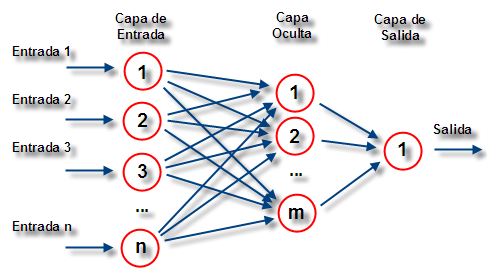
\includegraphics[scale=1]{img/rna.png}
			\caption{Red Neuronal Artificial}
			\label{fig:rna}
		\end{figure}

		Con el objetivo de lograr el aprendizaje de las redes neuronales, antes de enfrentarlas a un problema real, se requiere un proceso previo de entrenamiento que nos asegure que van a tener una buena capacidad de predicción para todos los casos, es decir, que el modelado sea eficaz.\\
		
		La Figura \ref{fig:func_rna} muestra gráficamente el funcionamiento de una RNA.\\
		
		\begin{figure}[h]
			\centering
			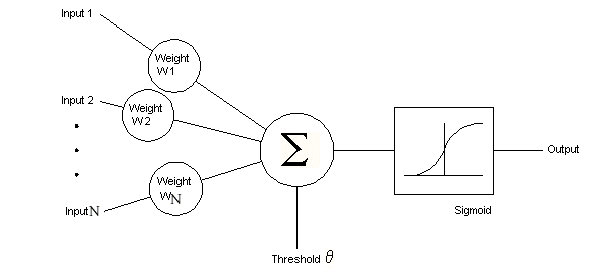
\includegraphics[scale=0.5]{img/rna_pesos.png}
			\caption{Funcionamiento de una Red Neuronal Artificial}
			\label{fig:func_rna}
		\end{figure}
		
		En 1988, el Estudio sobre Redes Neuronales realizado por DARPA\footnote{Defense Advanced Research Projects Agency (Agencia de Investigación de Proyectos Avanzados de Defensa) es una agencia del Departamento de Defensa de los Estados Unidos responsable del desarrollo de nuevas tecnologías para uso militar.} listaba varias aplicaciones con redes neuronales. Dicho estudio sirvió para que saliesen otras aplicaciones comerciales, incluyendo un pequeño reconocedor de palabras, un monitor de procesos o un clasificador de sonar.\\
		
		Las Redes Neuronales se han aplicado, además, en otros campos desde que DARPA escribió su informe. La siguiente lista contiene algunos de los campos en los que se utilizan actualmente las redes neuronales:
		
		\begin{itemize}
			\item Aeromodelismo espacial: simulación de vuelos, detección de fallos en componentes, etc.
			\item Automoción: sistemas de guía automáticos, análisis de garantías, etc.
			\item Banca: evaluación de tarjetas de crédito, etc.
			\item Defensa: búsqueda de objetivos, compresión de datos, extracción de características y supresión de ruidos, etc.
			\item Electrónica: predicción de códigos de secuencia, chip en circuitos integrados, etc.
			\item Entretenimiento: animaciones, efectos especiales, etc.
			\item Financias: análisis de uso de créditos, predicción de precios, etc.
			\item Manufactorías: control de procesos, diseño de productos, etc.
			\item Medicina: análisis de células cancerígenas, optimización de tiempos en trasplantes, etc.
			\item Robótica: control de trayectorias, controladores y manipuladores, sistemas de visión, etc.
		\end{itemize}
		
		\subsection{Regresión ordinal}
		
			La regresión ordinal (RO) permite asignar una métrica óptima a los regresores discretos de un modelo de regresión múltiple. Se trata, en síntesis, de elegir la recodificación de los predictores de acuerdo con una métrica ordinal tal, que se optimice el ajuste del modelo. De este modo, se extrae de cada regresor su mayor capacidad predictiva posible mediante una recodificación óptima de sus posibles valores en una nueva escala de naturaleza ordinal.
			
		\subsection{Algoritmo Resilient Backpropagation (RPROP)}
	
			\textit{Resilent backpropagation} (RPROP) \cite{RPROP} es una técnica de optimización robusta basada en el gradiente, que ha sido comúnmente utilizada para el entrenamiento de redes neuronales artificiales. Se basa en el uso de un valor de velocidad de avance del algoritmo para la actualización de cada parámetro del modelo.\\
	
			RPROP es una técnica ampliamente utilizada para el entrenamiento supervisado de redes neuronales artificiales tipo perceptrón multicapa, cuyo proceso de búsqueda es guiado por la primera derivada de la función $f(x)$; en este caso, $f'(x)$ es una medida de la diferencia entre la salida propuesta por la red neuronal y el valor esperado. RPROP difiere de la técnica clásica de propagación, hacia atrás, del error (o algoritmo \textit{backpropagation}) en que las derivadas parciales de la función error sólo son usadas para determinar el sentido en que deben ser corregidos los pesos de la red pero no las magnitudes de los ajustes. Los algoritmos basados en \textit{backpropagation} modifican los valores de los parámetros proporcionalmente al gradiente de la función de error, de tal forma que en regiones donde el gradiente tiende a ser plano el algoritmo avanza lentamente; esta modificación se hace con RPROP a través de un único parámetro que controla la velocidad de avance del algoritmo.\\
			
			Para comprender mejor el funcionamiento que tiene, las ecuaciones \ref{rprop1} y \ref{rprop2} muestran el funcionamiento de esta técnica:\\
			
			\begin{equation}
				\Delta w_{ij} (t) =
				\begin{cases}
					{ -\Delta p_{ij},} & \mbox{ si } \frac{ \partial E}{ \partial w_{ij}} > 0 \\
					{ +\Delta p_{ij},} & \mbox{ si } \frac{ \partial E}{ \partial w_{ij}} < 0 \\
					0, & \mbox{ si } \frac{ \partial E}{ \partial w_{ij}} = 0
				\end{cases}
				\label{rprop1}
			\end{equation}
				
			\begin{equation}
				\Delta p_{ij} (t) = 
				\begin{cases}
					{ \alpha^+ \cdot{} \Delta w_{ij}(t-1),} & \mbox{ si } \frac{ \partial E}{ \partial w_{ij}}(t-1) \cdot{} \frac{ \partial E}{ \partial w_{ij}}(t) > 0 \\
					{ \alpha^- \cdot{} \Delta w_{ij}(t-1),} & \mbox{ si } \frac{ \partial E}{ \partial w_{ij}}(t-1) \cdot{} \frac{ \partial E}{ \partial w_{ij}}(t) < 0 \\
					\Delta w_{ij}(t-1), & \mbox{ si } \frac{ \partial E}{ \partial w_{ij}}(t-1) \cdot{} \frac{ \partial E}{ \partial w_{ij}}(t) = 0
				\end{cases}
				\label{rprop2}
			\end{equation}
			
			Siendo,
			\begin{tabbing}
			\hspace{1 cm}\=\kill
			 \> $ w_ij $ los pesos o coeficientes del modelo,\\
			 \> $ t $ el instante de tiempo,\\
			 \> $ p_ij $ la actualización o cambio de los pesos,\\
			 \> $ E $ la entropía,\\
			 \> $ \alpha $ el rango de aprendizaje.
			\end{tabbing}
			
			Por otra parte, los parámetros obtenidos experimentalmente que se utilizan son,
			\begin{tabbing}
			\hspace{1 cm}\=\kill
			 \> $ \alpha^+ = 1.2, $\\ 
			 \> $ \alpha^- = 0.5, $\\ 
			 \> $ \Delta w(0) = 0.5, $\\ 
			 \> $ \Delta w(t)_{max} = 50, $\\ 
			 \> $ \Delta w(t)_{min} = 0 $
			\end{tabbing}
	
		\subsection{Algoritmo iRPROP+ (RPROP mejorado)}
	
			La variante de RPROP, iRProp+ \cite{iRPROP+}, añade un paso de vuelta atrás al algoritmo, que permite evitar los óptimos locales. La idea es que, cuando el cambio en un parámetro de la red haya producido un aumento del valor de la función de error, vuelva al estado anterior antes de producirse dicho cambio. De esta forma, se tienen las ecuaciones:\\
			
			\begin{equation}
				\Delta w_{ij} (t) = 
				\begin{cases}
					{ \alpha^+ \cdot{} \Delta w_{ij}(t-1),} & \mbox{si } \frac{ \partial E}{ \partial w_{ij}}(t-1) \cdot{} \frac{ \partial E}{ \partial w_{ij}}(t) > 0 \nonumber \\
					{ \Delta w_{ij}(t-1)-\Delta w_{ij}(t-2),} & \mbox{si } \frac{ \partial E}{ \partial w_{ij}}(t-1) \cdot{} \frac{ \partial E}{ \partial w_{ij}}(t) < 0 \nonumber \\
					& \mbox{ y } E(t) > E(t-1) \\
					\Delta w_{ij}(t-1), & \mbox{si } \frac{ \partial E}{ \partial w_{ij}}(t-1) \cdot{} \frac{ \partial E}{ \partial w_{ij}}(t) = 0 \nonumber
				\end{cases}
				\label{irprop+}
			\end{equation}
	
		\subsection{Redes Neuronales basadas en el modelo Proportional Odd Model (POM)}

			Para poder utilizar el algoritmo iRProp+ para regresión ordinal, nos vamos a basar en el modelo \textit{Proportional Odd Model} (POM) \cite{Mcc80}.\\

			Este modelo de regresión ordinal entra dentro del grupo de modelos de umbral, que se basan en suponer que la respuesta ordinal está asociada a una variable artificial medida en escala continua y modelada mediante intervalos de clase sobre la recta real. La mayoría de estos modelos se pueden representar mediante una función de rango $f(x)$ la cual transforma el vector de variables de entrada en valores de la recta real y un conjunto de umbrales $\left\{ \beta_0,\cdots,\beta_J \right\} $ que delimitan las categorías en esta recta. Diferentes formas de esta función de rango proporcionan modelos de clasificación ordinal como los que se han mencionado en el capítulo de Introducción.\\

			Bajo un punto de vista probabilístico, el modelo POM \cite{Mcc80} es el método estadístico básico de regresión ordinal y puede considerarse también como un modelo de umbral, donde $f(x)$ es una combinación lineal ponderada de las variables de entrada.\\

			La idea fundamental de este proyecto es basarnos en dicho modelo probabilístico para poder definir una red neuronal para regresión ordinal y utilizar una modificación del algoritmo iRProp+ (por su mayor eficiencia y eficacia) para optimizar los parámetros del modelo.\\
		
		\subsection{Medidas de rendimiento}
		
			Para comprobar que los resultados obtenidos después del entrenamiento y la simulación de una red neuronal artificial son buenos, es decir, que los resultados obtenidos al aplicar un algoritmo específico, se corresponden con un buen clasificador; existen unas medidas que se utilizan para poder ver la calidad o eficiencia de los resultados.\\
			
			Algunos de estas medidas se mencionarán y explicarán a continuación. Aunque existen más, estas son las más relevantes para el tema concreto que se está tratando que es la regresión ordinal mediante redes neuronales artificiales.
		
			\subsubsection{Matriz de confusión}
			
			Una matriz de confusión contiene información acerca de las clasificaciones actuales o predichas realizadas por un sistema de clasificación. El rendimiento de tales sistemas se evalúa, normalmente, usando los datos de esta matriz. La Tabla \ref{tabla_matriz_confusion} muestra la matriz de confusión para un clasificador de dos clases.\\
			
			\begin{table}[h]
				\centering
				\begin{tabular}{cc|c|c|c}
					\cline{3-4}
					& & \multicolumn{2}{|c|}{Predicho} \\ \cline{3-4}
					& & Negativo & Positivo \\ \cline{1-4}
					\multicolumn{1}{|c|}{\multirow{2}{*}{Actual}} &
					\multicolumn{1}{|c|}{Negativo} & a & b &     \\ \cline{2-4}
					\multicolumn{1}{|c|}{}                        &
					\multicolumn{1}{|c|}{Positivo} & c & d &     \\ \cline{1-4}
				\end{tabular}
				\caption{Matriz de confusión}
				\label{tabla_matriz_confusion}
			\end{table}
			
			Las entradas de la matriz de confusión tienen el siguiente significado en el contexto de nuestro estudio:

			\begin{itemize}
				\item a es el número de predicciones \textbf{correctas} en la que una instancia es negativa.
				\item b es el número de predicciones \textbf{incorrectas} en la que una instancia es positiva.
				\item c es el número de predicciones \textbf{incorrectas} en la que una instancia es negativa.
				\item d es el número de predicciones \textbf{correctas} en la que una instancia es positiva.
			\end{itemize}

			En el campo de la Inteligencia Artificial, una matriz de confusión es una herramienta de visualización usada normalmente en aprendizaje supervisado (en aprendizaje no supervisado se le suele llamar matriz de coincidencias). Uno de los beneficios de usar una matriz de confusión es, que es muy fácil ver si el sistema distingue entre las dos clases.\\
			
			Los siguientes términos son importantes para la comprensión de los valores de la matriz de confusión del ejemplo:\\

    		La precisión (AC - accuracy) es la proporción del número total de predicciones que fueron correctas. Se calcula usando la siguiente ecuación:\\

			\begin{equation}
				AC = \frac{a+d}{a+b+c+d}
				\label{AC}
			\end{equation}
			\\

		    Un verdadero positivo (TP - true possitive) es la proporción de casos positivos que se identificaron correctamente, se calcula mediante la siguiente ecuación:\\

			\begin{equation}
				TP = \frac{d}{c+d}
				\label{TP}
			\end{equation}
			\\

			Un falso positivo (FP - false possitive) es la proporción de casos negativos que se clasificaron incorrectamente como positivos, se calcula mediante la siguiente ecuación:\\

			\begin{equation}
				FP = \frac{b}{a+b}
				\label{FP}
			\end{equation}
			\\

			Un verdadero negativo (TN - true negative) se define como la proporción de casos negativos que se clasificaron correctamente, se calcula mediante la siguiente ecuación:\\

			\begin{equation}
				TN = \frac{a}{a+b}
				\label{TN}
			\end{equation}
			\\

		    Un falso negativo (FN- false negative) es la proporción de casos positivos que fueron incorrectamente clasificados como negativos, se calcula mediante la siguiente ecuación:\\

			\begin{equation}
				FN = \frac{c}{c+d}
				\label{FN}
			\end{equation}
			\\

			Por último, la proporción (P) es la proporción de los casos positivos predichos que fueron correctos, se calcula mediante la siguiente ecuación:\\

			\begin{equation}
				P = \frac{d}{b+d}
				\label{P}
			\end{equation}
			\\
		
			\subsubsection{Ratio Correctamente Clasificado (Correctly Classified Rate (CCR))}
			
			Cuando se tiene más de dos clases en el modelo se calcula la precisión o CCR, que es el número de elementos en la diagonal principal de la matriz de confusión, es decir, la suma del número de predicciones correctas en la que una instancia es negativa más el número de predicciones correctas en la que una instancia es positiva, dividido por el número total de elementos de la matriz.\\
			
			Anteriormente se ha visto como la precisión o AC, pero generalizando para este caso en concreto, se puede decir que corresponde a la siguiente ecuación:\\
			
			\begin{equation}
				CCR = \frac{\text{nº de bien clasificados}}{\text{nº total de patrones}}
				\label{CCR}
			\end{equation}
			\\
		
			\subsubsection{Error Absoluto Medio (Mean Absolute Error (MAE))}
			
			En estadística, el error absoluto medio es una cantidad usada para medir como de buenos son los pronósticos o predicciones de los resultados. El error absoluto medio (MAE) viene dado por la siguiente ecuación:
			
			\begin{equation}
				MAE = \frac{1}{n} \sum_{i=1}^n{\left |{f_i-y_i}\right |} = \sum_{i=1}^n{\left |{e_i}\right |}
				\label{MAE}
			\end{equation}
			\\
			
			Como su propio nombre indica, el error absoluto medio es una media de los errores absolutos, $ e_i = f_i-y_i $, donde $ f_i $ es la predicción e $ y_i $ es el valor verdadero. Existe una notación alternativa en la que se puede incluir frecuencias relativas como factores de peso.\\

			El error absoluto medio es una medida común de pronóstico de errores en análisis temporales de series, donde el término ``error absoluto medio" se utiliza en algunas ocasiones confundiéndolo con la definición más estandarizada de desviación media absoluta.\\

			El MAE mide la magnitud media de los errores en un conjunto de pronóstico, sin considerar su dirección. Así, se puede decir que mide la precisión para variables continuas.\\
			
			También es una medida específica para clasificación ordinal. Donde se realiza el sumatorio de los  errores cometidos por un clasificador en valor absoluto asignando una etiqueta numérica a cada clase. Para ahorrar coste computacional, el error absoluto medio también se puede calcular en base a la matriz de confusión explicada anteriormente, multiplicando ésta por una matriz de costes del estilo a la mostrada:
			
			\begin{equation}
				MP = 
					\begin{bmatrix}
						{0}&{1}&{2}&{3}\\
						{1}&{0}&{1}&{2}\\
						{2}&{1}&{0}&{1}\\
						{3}&{2}&{1}&{0}
					\end{bmatrix}
				\label{matriz_pesos}
			\end{equation}
			\\
			
			Multiplicando elemento a elemento, no de forma matricial, la matriz de confusión por esta otra matriz de pesos, resultará una matriz de errores absolutos. Dándole un peso proporcional a la distancia entre aquellos elementos mal clasificados. En este momento, haciendo el sumatorio de todos los elementos de la matriz y dividiéndolo por el número total de elementos, se obtendrá el MAE. La siguiente ecuación muestra lo explicado anteriormente:
			
			\begin{equation}
				MAE = \frac{\sum{(MC \cdot{} MP)}}{TOTAL}
				\label{matriz_mae}
			\end{equation}
			\\
			
			\subsubsection{Error Cuadrático Medio (Mean Square Error (MSE))}
			
			En estadística, el error cuadrático medio o MSE de un estimador es uno de los posibles caminos para cuantificar la diferencia entre un estimador y el valor verdadero de la cantidad que se va a estimar, es decir, es la media aritmética de los cuadrados de las desviaciones del estimador $\hat{\theta}$ respecto al valor verdadero del estadístico que se trata de estimar.\\

			Se diferencia de la varianza en que, en ésta, las desviaciones son con respecto a la media aritmética. Lógicamente, cuando el estimador sea insesgado, el error cuadrático medio será igual a la varianza.\\
			
			El MSE de un estimador con respecto al parámetro estimado $\hat{\theta}$ se define como:

			\begin{equation}
				MSE(\hat{\theta}) = E[(\hat{\theta}-\theta)^2]
				\label{estimator_mse}
			\end{equation}
			\\

			El MSE también se puede calcular sumando la varianza al cuadrado del sesgo o \textit{bias} del estimador:

			\begin{equation}
				MSE(\hat{\theta}) = Var(\hat{\theta})+\left(Bias(\hat{\theta},\theta)\right)^2
				\label{varianza_mse}
			\end{equation}
			\\
		
	\section{Matlab}
	
		MATLAB es un lenguaje de computación de alto nivel y un entorno interactivo para desarrollo de algoritmos, visualización de datos, análisis de datos y cálculo numérico. Con MATLAB, se puede resolver problemas de cálculo más rápidamente que con lenguajes de programación tradicionales, tales como C, C++ o Fortran.\\
		
		El lenguaje de MATLAB incluye operaciones vectoriales y matriciales que son fundamentales para resolver los problemas científicos y de ingeniería. Agiliza tanto el desarrollo como la ejecución.\\

		Con el lenguaje de MATLAB, se puede programar y desarrollar algoritmos más rápidamente que con los lenguajes tradicionales porque ya no hay que realizar tareas administrativas de bajo nivel, tales como declarar variables, especificar tipos de datos o asignar memoria. En muchos casos, MATLAB elimina la necesidad de bucles ``for", o condiciones explícitas ``if". Por ello, una línea de código de MATLAB generalmente reemplaza a varias líneas de código en C/C++, Fortran o JAVA.\\

		Al mismo tiempo, MATLAB ofrece todas las características de los lenguajes de programación tradicionales, que incluyen operadores aritméticos, control de flujo, estructuras de datos, tipos de datos, programación orientada a objetos (OOP) y depuración.\\
		
		MATLAB permite ejecutar comandos o grupos de comandos uno a uno, sin compilar ni enlazar, y repetir su ejecución hasta lograr la solución óptima.\\
		
		También ofrece todas las funciones gráficas necesarias para visualizar datos de ingeniería y científicos. Incluye funciones de representación de diagramas bidimensionales y tridimensionales, visualización de volumen tridimensional, herramientas para crear diagramas en forma interactiva y la posibilidad de exportar los resultadas a los formatos gráficos más conocidos. Se puede personalizar los diagramas añadiendo varios ejes, cambiando los colores de las líneas y marcadores, añadiendo anotaciones, ecuaciones LaTeX, leyendas y trazando formas.\\
		
		MATLAB es un software multiplataforma y eso facilita que cualquiera pueda hacer desarrollos en Matlab en su propio sistema operativo.
	
		\subsection{Toolbox \textit{nnet} (Neural Network Toolbox)}
		
			Neural Network Toolbox proporciona herramientas para el diseño, implementación, visualización y simulación de redes neuronales artificiales. Las redes neuronales se utilizan para aplicaciones donde el análisis formal es difícil o imposible, tales como reconocimiento de patrones o los sistemas no lineales de identificación y control. El toolbox soporta redes con conexiones hacia adelante o ``feedforward", redes de base radial, redes dinámicas, mapas auto-organizados u otros paradigmas de red probadas.\\

			Las redes neuronales se componen de elementos simples funcionando en paralelo. Estos elementos están inspirados en los  sistemas nerviosos biológicos. Al igual que en la naturaleza, las conexiones entre los elementos determinan en gran medida la función de red. Se puede entrenar una red neuronal para realizar una función en particular, mediante el ajuste de los valores de las conexiones (pesos) entre los elementos.\\

			Por lo general, las redes neuronales se ajustan o se entrenan de modo que una determinada entrada conducirá a una salida específica.
			
		\subsection{Interfaces gráficas con Matlab}
			
			Matlab proporciona la posibilidad de crear Interfaces Gráficas de Usuario (GUI\footnote{Graphical User Interface.}) de varias formas, por ejemplo, a través de librerías de interfaz externas que permiten implementarlas escritas en C/C++, JAVA y Fortran o utilizando su aplicación gráfica para la creación de interfaces o realizando la interfaz programándola directamente a través de ficheros MAT.\\
			
			Una Interfaz Gráfica de Usuario es una exposición gráfica en una o más ventanas que contiene controles, componentes de llamada, que permite al usuario realizar tareas interactivas con un sistema. El usuario de la GUI no tiene porque crear un script o escribir comandos en la línea de comandos para realizar las tareas. Ésto ayuda a los usuarios a comprender los detalles de cómo se realizan las tareas.\\
			
			Los componentes que puede incluir una GUI pueden ser tales como menús, barras de herramientas, botones de varios tipos, listas de selección, etc. Las GUIs creadas usando las herramientas de MATLAB pueden realizar cualquier tipo de computación, como por ejemplo, leer y escribir en ficheros externos, comunicarse con otras GUIs o mostrar datos como gráficos.\\
			
			Como se ha comentado antes, se podrán realizar GUIs con MATLAB de dos maneras posibles:
			
			\begin{itemize}
				\item Usando la herramienta para creación de interfaces gráficas que contiene llamada GUIDE (GUI Development Environment)\footnote{Entorno de Desarrollo para GUI. La aplicación gráfica es muy simple y se asemeja mucho a la aplicación QTCreator para creación de interfaces gráficas con C++.}.
				\item O creando los ficheros de código fuente que generarán las GUIs como funciones o scripts (a esta técnica se la denomina \textit{construcción programada de GUIs}).
			\end{itemize}

	\chapter{Restricciones}
	
	En este capítulo se expondrán todas las restricciones, o factores limitativos, existentes en el ámbito del diseño y que condicionan la elección de una u otra alternativa. Los factores limitativos pueden estructurarse en dos grupos:
	
	\begin{itemize}
		\item \textbf{Factores dato:} son aquellos que no pueden ser modificados durante el transcurso del proyecto, como puede ser el presupuesto económico asignado al proyecto o la duración estimada del mismo.
		\item \textbf{Factores estratégicos:} representan variables de diseño que permiten la elección entre diferentes alternativas por parte del ingeniero. En función de la opción escogida, podrá alterarse el proceso de desarrollo y el propio producto final obtenido, con lo que resultará necesario analizar las posibilidades existentes en las primeras etapas del proceso.
	\end{itemize}
	
	\section{Factores dato}
	
		En el desarrollo de este proyecto se van a considerar los siguientes factores dato impuestos por el tipo de proyecto:
	
		\begin{itemize}
			\item \textbf{Restricciones humanas:} al ser éste un proyecto final de carrera, este factor lo condiciona el director de proyecto (perteneciente al grupo de investigación AYRNA), restringiendo el proyecto a un número determinado de personas. En nuestro caso, un solo alumno para el desarrollo del mismo.
			\item \textbf{Restricciones temporales:} estará condicionado al cumplimiento de los objetivos previamente establecidos, aunque por lo general, se suele establecer limitaciones con el fin de no demorar en exceso la presentación del Proyecto. En este caso, el tiempo de elaboración de este Proyecto se espera que no sobrepase la convocatoria de septiembre del curso 2010/2011, a expensas de no sufrir contratiempos.
			\item \textbf{Restricciones hardware:} dado a la cantidad de cálculos que realizarán los algoritmos desarrollados, desde el cliente nos imponen ciertas restricciones hardware (como la potencia de los equipos en los que se utilizará el sistema) a tener en cuenta a la hora de elegir ciertos parámetros en el futuro de diseño de la aplicación.
			\item \textbf{Restricciones software:} según las características del proyecto y el fin que tendrá, meramente investigador. No se impone un software específico ni un lenguaje de programación en especial, pero sí que tenga la suficiente potencia para desarrollar el proyecto.
		\end{itemize}
		
	\section{Factores estratégicos}
	
		Los principales factores estratégicos que afectan al presente proyecto, así como los diferentes motivos que justifican la elección realizada en cada restricción, son los que se comentan a continuación:
		
		\begin{itemize}
			\item Los algoritmos que se desea desarrollar deberán estar bien modularizados, de manera que permita de manera fácil y con la mayor agilidad posible la realización de futuras modificaciones y ampliaciones que puedan considerarse necesarias.
			\item Los algoritmos se desarrollarán en el entorno de desarrollo Matlab, porque la potencia que ofrece este software de desarrollo matemático y la utilidad de tener a disposición un Toolbox sobre redes neuronales que facilitan la elaboración del proyecto.
			\item Para la elaboración de la documentación en \LaTeX{} se utilizará el editor Texmaker, ya que es de libre distribución.
			\item Para la elaboración de cualquier tipo de diagramas se hará uso de la herramienta Día, disponible en libre distribución para los distintos sistemas operativos.
		\end{itemize}

	\chapter{Recursos}
	
	En este capítulo se expondrán de forma clara y concisa los recursos humanos y materiales necesarios para este proyecto. Los recursos se definen como aquellos medios de los que se dispone para abordar el proceso de desarrollo del proyecto. El análisis de los recursos existentes se realizará atendiendo a una doble perspectiva:
	
	\begin{itemize}
		\item \textbf{Recursos humanos:} son aquellos que están constituidos por toda persona que intervenga en el proceso de desarrollo del sistema.
		\item \textbf{Recursos materiales:} son aquellos que pueden definirse como el conjunto de todas las entidades no animadas que permiten realizar el proceso de desarrollo de la aplicación, así como la generación de la documentación relativa a la misma.
	\end{itemize}
	
	\section{Recursos humanos}
	
		El conjunto de personas que intervendrán durante el proceso de desarrollo del presente proyecto se muestran a continuación:
	
		\begin{itemize}
			\item \textbf{Directores:}
			\begin{itemize}
				\item Prof. Dr. Pedro Antonio Gutiérrez Peña.\\
	
				Profesor Ayudante Doctor del Dpto. de Informática y Análisis Numérico y miembro investigador del grupo AYRNA.
	
				\item Prof. Dr. César Hervás Martínez.\\

				Catedrático del Dpto. de Informática y Análisis Numérico y director del grupo AYRNA.
			\end{itemize}
			
			Los directores se encargarán de supervisar las tareas de desarrollo para comprobar que los resultados obtenidos se corresponden con los requisitos planteados. Además, facilitarán aquellos recursos materiales que resulten necesarios para abordar con éxito el proceso de desarrollo.
		
			\item \textbf{Autor:}
			\begin{itemize}
				\item Raúl Pérula Martínez.\\
	
				Ingeniero Técnico Informático de Sistemas.
			\end{itemize}
		\end{itemize}
	
	\section{Recursos materiales}
		
		\subsection{Recursos software}
			
			\begin{itemize}
				\item Sistema operativo Ubuntu 10.04.
				\item Lenguaje de programación y herramienta MATLAB 2010a.
				\item Lenguaje \LaTeX{} para la realización de la documentación.
				\item Texmaker 2.1 como editor de documentos \LaTeX{}.
				\item Programa de edición de diagramas, dia 0.97.1.
			\end{itemize}
			
		\subsection{Recursos hardware}
			
			Equipo portátil con las siguiente características técnicas:
			
			\begin{itemize}
				\item Procesador Intel Core 2 Duo T7300 (Santa Rosa) a 2 GHz (4 MB memoria caché L2).
				\item 2048 MB de memoria RAM.
				\item Disco duro de 120 GB.
			\end{itemize}

	\chapter{Especificación del sistema}
	
	En los capítulos anteriores se ha proporcionado una visión general del problema a resolver. En este capítulo, dedicado a la especificación, se va a detallar el funcionamiento del algoritmo de regresión ordinal basado en redes neuronales artificiales y se realizará un análisis del coste computacional de sus fases atendiendo a posibles optimizaciones.
	
	\section{Algoritmo de Regresión Ordinal ORNNet}
	
		En esta sección se explicará el funcionamiento detallado del algoritmo a implementar.\\
		
		El modelo de la red neuronal se basa en una capa de entrada, dos capas ocultas y una capa de salida. La capa de entrada tomará los valores de entrenamiento de entrada ($x_1, x_2, ..., x_i$) que para pasar a la siguiente capa obtendrá nuevos valores ($B_1, B_2, ..., B_i$), cambiando los valores de los pesos ($w_1, w_2, ..., w_i$). Para actualizar estos valores se utilizará una función de transferencia (sigmoide), por ejemplo, una \textit{logsig} o \textit{tansig}. La primera capa oculta obtendrá los nuevos valores a partir de los datos elegidos, en cambio, la segunda capa oculta, que tendrá solo una neurona, obtendrá los valores de la capa anterior y no tendrá \textit{bias}. Esta capa tendrá como función de transferencia fija del tipo \textit{purelin}. Por último, para obtener los valores de la capa de salida, que tendrá el mismo número de neuronas que la capa de entrada, se pondrá el valor de los pesos fijo a 1 y se utilizará la función de transferencia \textit{logsig}. Una de las condiciones que hay para la capa de salida es que el valor de las \textit{bias} tiene que mantener el orden, es decir, $\beta^1_0< \beta^2_0< \cdots < \beta^{J-1}_0$. Una vez obtenida la salida se hará una transformación de los valores para poder tratarlos.\\
		
		La Figura \ref{fig:ORNNet} muestra gráficamente dicho funcionamiento.\\
		
		\begin{figure}[h]
			\centering
			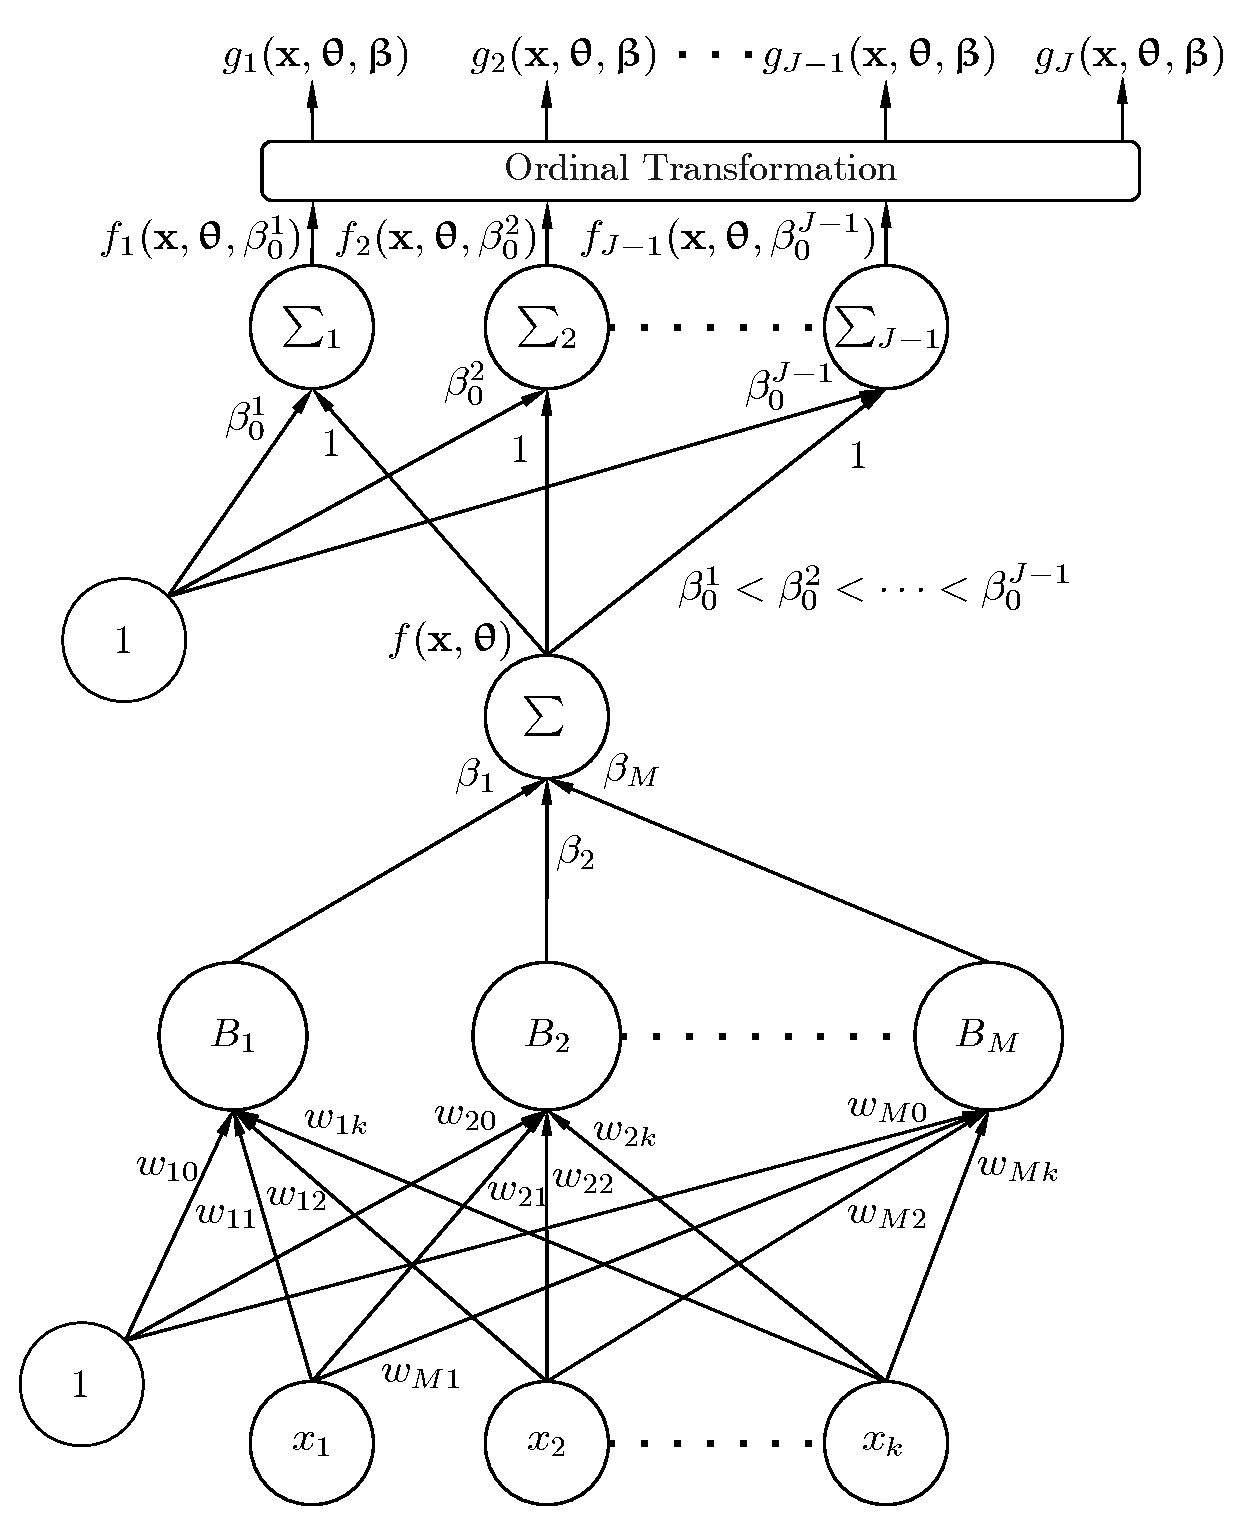
\includegraphics[scale=0.5]{img/ORNNet.pdf}
			\caption{Funcionamiento del algoritmo para redes neuronales artificiales ORNNet.}
			\label{fig:ORNNet}
		\end{figure}
		
		La mayoría de los modelos de regresión ordinal se representan como en la ecuación \ref{GeneralOR}.\\
		
		\begin{equation}
			C(\mathbf{x})=
			\begin{cases}
				c_1, & \text{si $f(\mathbf{x},{\boldsymbol \theta})\le \beta^1_0$}\\
				c_2, & \text{si $\beta^1_0<f(\mathbf{x},{\boldsymbol \theta})\le \beta^2_0$}\\
				\cdots\\
				c_J, & \text{si $f(\mathbf{x},{\boldsymbol \theta})>\beta^{J-1}_0$}
			\end{cases}
			\label{GeneralOR}
		\end{equation}\\

		siendo $c_1, c_2, ..., c_J$ las clases ordenadas, $\beta^1_0< \beta^2_0< \cdots < \beta^{J-1}_0$ los sesgos o \textit{bias} de las funciones discriminantes y $f(\mathbf{x},{\boldsymbol \theta})$ la función de ranking discriminante (en este caso, no lineal).\\
		
		Nuestro modelo, que llamaremos ORNNet, es similar al modelo POM\footnote{Proportional Odds Model, modelo explicado en el capítulo de Antecedentes.}, pero usando transformaciones básicas no lineales de las entradas en lugar de las variables de entrada. De este modo, las funciones discriminantes a utilizar son ahora:\\
		
		\begin{equation}
			f_l(\mathbf{x},{\boldsymbol \theta},\beta^l_0)=f(\mathbf{x},{\boldsymbol \theta})-\beta^l_0;\;1\le l\le J-1
			\label{funcion_modelo}
		\end{equation}\\
		
		siendo $f(\mathbf{x},{\boldsymbol \theta})$ la función de base del modelo, como por ejemplo, un sumatorio de transformaciones no lineales de las variables de entrada:\\
		
		\begin{equation}
			f(\mathbf{x},{\boldsymbol \theta})=\sum_{i=1}^M \beta_i B_i(\mathbf{x},\mathbf{w}_i)
			\label{NL}
		\end{equation}\\
		
		donde $B_i(x,w_i)$ son las funciones de base, que este proyectos se han utilizado del tipo \textit{logsig}, \textit{tansig} y \textit{purelin}.\\
		
		Haciendo uso del modelo POM, las probabilidades acumuladas, las posibilidades acumuladas\footnote{Cumulative odds.} y los logits acumulados serían:\\
		
		\begin{eqnarray}
			P(Y\le l) = p_1+\cdots+p_l \\
			odds(Y\le l) =\frac{P(Y\le l)}{1-P(Y\le l)}\\
			logit(Y\le l)=\ln \left(\frac{P(Y\le l)}{1-P(Y\le l)}\right)
			\label{POM_odds}
		\end{eqnarray}\\
		
		para $1\le l\le J-1$.\\

		Y en el modelo de ORNNet:\\
		
		\begin{eqnarray}
			& logit(Y\le l)=f_l(\mathbf{x},{\boldsymbol \theta},\beta^l_0)=f(\mathbf{x},{\boldsymbol \theta})-\beta^l_0;\; & 1\le l\le J-1\\
			& P(Y\le l)=\frac{1}{1+\exp(f(\mathbf{x},{\boldsymbol \theta)}-\beta^l_0)};\; & 1\le l\le J-1\\
			& P(Y\le J)=1 & 
			\label{ORNNet_odds}
		\end{eqnarray}\\

		Esto permite expresar las probabilidades como:\\
		
		\begin{eqnarray}
			& P(Y=1)=g_{1}(\mathbf{x},\boldsymbol{\theta},{\boldsymbol \beta})=P(Y\le 1) \\
			& P(Y=l)=g_{l}(\mathbf{x},\boldsymbol{\theta},{\boldsymbol \beta})=P(Y\le l)-P(Y\le l-1)
			\label{probability}
		\end{eqnarray}\\
		
		donde $2 \leq l \leq J$.\\
		
		En el problema de clasificación ordinal, la medidas $x_{i}$, $i=1,2,...,k$, se toman de manera individual (o como un objeto) y éstos se clasifican en una de las $J$ clases en base a dichas mediciones. Se asume que $J$ es finito y que las medidas de $x_{i}$ son observaciones aleatorias de esas clases.\\
		
		Sea $D = \left\{(\mathbf{x}_{n}, \mathbf{y}_{n}); n=1,2,...,N\right\}$ un conjunto de datos de entrenamiento, donde $\mathbf{x}_{n} =(x_{1n},...,x_{kn})$ es el vector de mediciones tomando valores en $\mathbf{\Omega} \subset {\mathbb R}^{k}$, e $\mathbf{y}_{n}$ el nivel de clase o etiqueta del $n$-ésimo individuo. Se adoptará la técnica más común para representar niveles de clases usando un vector de codificación ``$1$-de-$J$'', $\mathbf{y}=\left(y^{(1)} ,y^{(2)} ,...,y^{(J)} \right)$, tal que $y^{(l)} =1$ si $\mathbf{x}$ corresponde a un elemento perteneciente a la clase $l$ y, en otro caso, a $y^{(l)} =0$.\\
		
		La función que se usará para evaluar una red ORNNet es la del error cuadrático medio (MSE) que viene expresada a continuación:\\
		
		\begin{eqnarray}
			l(\boldsymbol{\beta},\boldsymbol{\theta})=-\frac{1}{N}\sum_{n=1}^N \sum_{l=1}^J \left( g_{l}(\mathbf{x},\boldsymbol{\theta},{\boldsymbol \beta})-y_n^{(l)}\right)^2
			\label{eq:mse}
		\end{eqnarray}\\
		
		donde $\boldsymbol{\beta}=(\beta_0^1,...,\beta_0^{J-1})$ es el vector de sesgos o \textit{bias} y el modelo es:\\
		
		\begin{eqnarray}
			g_{1}(\mathbf{x},\boldsymbol{\theta},{\boldsymbol \beta})= \displaystyle \frac{1}{1+\exp(f_1(\mathbf{x},{\boldsymbol \theta},\beta^1_0))} \\
			g_{l}(\mathbf{x},\boldsymbol{\theta},{\boldsymbol \beta})= \displaystyle \frac{1}{1+\exp(f_l(\mathbf{x},{\boldsymbol \theta},\beta^l_0))}-\frac{1}{1+\exp(f_{l-1}(\mathbf{x},{\boldsymbol \theta},\beta^{l-1}_0))}  \\
			g_{J}(\mathbf{x},\boldsymbol{\theta},{\boldsymbol \beta})= \displaystyle 1-\frac{1}{1+\exp(f_{J-1}(\mathbf{x},{\boldsymbol \theta},\beta^{J-1}_0))}
			\label{modelo}
		\end{eqnarray}\\
		
		donde $l = 2,\dots,J-1$.\\
		
		Para el propósito que de este algoritmo, se ha realizado una adaptación del procedimiento para óptimos locales en regresión ordinal, $iRprop^{+}$, y la función del MSE (Ecuación \ref{eq:mse}). En este caso, el vector gradiente sigue la siguiente formulación.\\
		
		\begin{equation}
			\nabla l(\boldsymbol{\beta},\beta_1,\cdots,\beta_M, \mathbf{w}_1,\cdots,\mathbf{w}_M) = \left(\frac{\partial l}{\partial \boldsymbol{\beta}},\frac{\partial l}{\partial \beta_1},\cdots,\frac{\partial l}{\partial \beta_M},\frac{\partial l}{\partial \mathbf{w}_1},\cdots, \frac{\partial l}{\partial \mathbf{w}_M} \right) \nonumber
			\label{gradient_vector}
		\end{equation}\\
		
		donde $\beta_1,...,\beta_M$ y $w_1,...,w_M$ son los coeficientes de la función de base mostrada en la Figura \ref{fig:ORNNet}.\\

		Siendo $\eta$ alguno de los parámetros $\boldsymbol{\beta}$ o $\boldsymbol{\theta}$. Con lo que:\\
		
		\begin{eqnarray*}
			\frac{\partial l}{\partial \eta} & = &  \frac{1}{N} \sum_{n=1}^{N} \sum_{l=1}^{J} 2\cdot\left( g_{l}(\mathbf{x},\boldsymbol{\theta},{\boldsymbol \beta})-y_n^{(l)}\right)\cdot\frac{\partial g_l(\mathbf{x},{\boldsymbol \theta},{\boldsymbol \beta})}{\partial \eta}. \nonumber
			\label{derivada}
		\end{eqnarray*}\\
		
		Derivando ahora la función $g$:\\
		
		\begin{eqnarray*}
			\frac{\partial g_l(\mathbf{x},{\boldsymbol \theta},{\boldsymbol \beta})}{\partial \eta} & = &
			\begin{cases}
				\displaystyle \left( \frac{-e^{f_{1}}}{\left( 1+ e^{f_{1}} \right)^2}\right) \frac{\partial f_{1}}{\partial \eta},& l=1 \\
				\displaystyle \left( \frac{-e^{f_{l}}}{\left( 1+ e^{f_{l}} \right)^2}\right) \frac{\partial f_{l}}{\partial \eta} -\left( \frac{-e^{f_{l-1}}}{\left( 1+ e^{f_{l-1}} \right)^2}\right) \frac{\partial f_{l-1}}{\partial \eta}, & l=2,\cdots,J-1\\
				\displaystyle -\left( \frac{-e^{f_{J-1}}}{\left( 1+ e^{f_{J-1}} \right)^2}\right) \frac{\partial f_{J-1}}{\partial \eta}, & l=J
			\end{cases}
			\nonumber \\
			\label{derivada_g}
		\end{eqnarray*}\\
		
		donde $g_l(\mathbf{x},{\boldsymbol \theta},{\boldsymbol \beta})=g_l$ y $f_l(\mathbf{x},{\boldsymbol \theta},\beta^l_0)=f_l$.\\

		La siguiente expresión incluye las derivadas de los coeficientes para la capa de salida:\\
		
		\begin{eqnarray}
			& \displaystyle \frac{\partial f_{l}}{\partial \beta_{0}^{k}} = \left\{ \begin{array}{ll}
         0 & \mbox{$k \neq l$}\\
        -1 & \mbox{$k = l$} \end{array} \right. , \nonumber \\
& \displaystyle \frac{\partial f_{l}}{\partial \beta_{s}} = B_{s}(\mathbf{x},\mathbf{w}_s);\;1\le s\le M \nonumber
		\end{eqnarray}\\

		El gradiente para las capas ocultas dependerá del tipo de función base. Si $B_{s}(\mathbf{x},\mathbf{w}_s)$ son nodos sigmoidales; cuya ecuación es:\\
		
		\begin{eqnarray}
			B_{s}(\mathbf{x},\mathbf{w}_s) & = & \sigma\left(\sum_{i=1}^k w_{is} x_i\right), \sigma(x)=\frac{1}{1+e^{-x}}
		\end{eqnarray}\\

		Entonces,\\

		\begin{eqnarray}
			\frac{\partial l}{\partial \mathbf{w}_s} & = & \left(\frac{\partial f_{l}}{\partial w_{s1}}, \cdots, \frac{\partial f_{l}}{\partial w_{sk}}\right) \nonumber \\
			\frac{\partial f_{l}}{\partial w_{st}} & = & \beta_s^l\sigma'\left( \sum_{i=1}^k w_{is} x_i \right) x_t \nonumber
		\end{eqnarray}\\
		
		donde $l = 1, 2, \dots, J-1$, $t = 1, 2, \dots, k$ y $s = 1, 2, \dots, M$.
		
	\section{Descripción funcional del sistema}
	
		En esta sección, se describirá el sistema con detalle, haciendo uso de técnicas de modelado que mostrarán de un modo inequívoco cómo interviene el usuario en el sistema, cuáles son los ítems que componen el sistema y qué operaciones soportan estos ítems. Para ello, se empleará la metodología UML (Lenguaje Unificado de Modelado) \cite{UML}.\\
		
		UML es un lenguaje de modelado que mediante un determinado vocabulario y un conjunto de reglas es capaz de representar conceptual y físicamente un sistema. El motivo de escoger esta metodología es que incorpora técnicas sencillas que dan una visión más cercana de lo que el usuario espera obtener.
		
		\subsection{Valores de los diferentes parámetros que utiliza el sistema}

		Con respecto a los principales valores del conjunto de datos que se vaya a usar, el número de capas ocultas, las funciones de las capas ocultas, etc. serán valores que se decidirán en secciones posteriores, durante la experimentación o en cuanto se pueda evaluar el funcionamiento del módulo, de manera que se consiga una mejor solución.\\
		
		A continuación se describen los parámetros más comunes a definir por el usuario para el algoritmo o la creación de la red neuronal artificial:
		
		\begin{itemize}
			\item \textit{Conjunto de datos}: son los datos que se especificarán para que el sistema pueda funcionar y para que la red neuronal pueda entrenar y simular los resultados de salida.
			\begin{itemize}
				\item \textbf{Datos de entrada}: son los datos de entrada del sistema, éstos vendrán definidos para cada conjunto de datos con los que se pruebe el sistema y tendrán un formato ordinal.
				\item \textbf{Datos objetivos}: son los datos objetivo del sistema, éstos se utilizarán para comprobar cuanto de buena es la red neuronal y el algoritmo implementado conteniendo los resultados reales de la clasificación.
			\end{itemize}
			\item \textit{Número de neuronas en las capas ocultas}: este parámetro podrá ser variable en función de cuantas capas ocultas y cuantas neuronas se desee poner en la red neuronal, por defecto se establecerán dos capas en la que la primera capa oculta contendrá 20 neuronas por defecto y la segunda capa oculta, que será fija para el sistema, contendrá 1 neurona. Adicionalmente, se proporcionará la opción de calcular el número óptimo de neuronas que debería haber en las capas ocultas.
			\item \textit{Número de neuronas en la capa de salida}: este parámetro es fijo, ya que será el mismo número que haya en la entrada del sistema.
			\item \textit{Funciones de transferencia de las capas}: este parámetro podrá contener alguno de los siguientes valores: \textit{logsig}, \textit{tansig}, \textit{purelin}, \textit{softmax}; para las capas ocultas que se definan. Adicionalmente, para las capas fijas, la última capa de la capa oculta y la capa de salida, tendrán el valor de \textit{purelin} y \textit{logsig} respectivamente.
			\item \textit{Función de entrenamiento}: la función de entrenamiento que se usará en el sistema será la implementada para el algoritmo ORNNet que será una modificación del algoritmo visto con anterioridad iRProp+.
			\item \textit{Función de aprendizaje}: este parámetro vendrá por defecto en el sistema al crear la red neuronal y se utilizará el valor: \textit{learngdm}, la cual se basa en descenso de gradiente.
			\item \textit{Función de precisión}: para este parámetro también se usará el valor por defecto: \textit{mse}, aunque se podrá modificar en cuanto convenga. Los distintos valores que podrá tomar son: \textit{mse} y \textit{mae}.
		\end{itemize}

		\subsection{Diagramas de Casos de Uso}

		Para obtener el modelo de objetos del software a desarrollar, se partirá de un conjunto de casos de uso desde un alto nivel de abstracción hasta un nivel de detalle más elevado, pudiendo obtener de esta forma todos los requisitos necesarios y los objetos que conformarán el sistema. Un caso de uso especifica el comportamiento de un sistema o de una parte del mismo y es una descripción de un conjunto de secuencias de acciones, incluyendo variantes, que ejecuta un sistema para producir un resultado observable de valor para un actor.\\
		
		Los casos de uso se emplean para capturar el comportamiento deseado del sistema en desarrollo sin tener que especificar cómo se implementa ese comportamiento, además de proporcionar un medio para que los desarrolladores, los usuarios finales del sistema y los expertos del dominio lleguen a una comprensión común del sistema.

			\subsubsection{Perfiles de usuario}

			En el sistema de resolución de problemas de modelado se pueden distinguir distintos tipos de actores, un actor representa un conjunto coherente de roles que juegan los usuarios de los casos de uso al interactuar con él. Los actores pueden ser personas o sistemas externos, establecidos por la siguiente clasificación:
			
			\begin{itemize}
				\item \textit{Principales:} personas que usan el sistema, serán los usuarios del sistema. Este proyecto no se basa en la interacción con el usuario del sistema ya que retoma más importancia la implementación y la obtención de resultados del algoritmo propuesto, no obstante, existirá una interfaz gráfica con la que el usuario podrá interactuar. El usuario podrá ejecutar el algoritmo y obtener los resultados. Para alcanzar dicho fin, el usuario tendrá que introducir unos parámetros de entrada, es decir, un conjunto de datos de entrada y de objetivos para el entrenamiento y el testeo de la red neuronal. Una vez especificados, habrá que crear la red neuronal y seguidamente realizar el entrenamiento y la simulación de la misma. Por último, tendrá que recoger las salidas. Las personas que usarán el sistema serán aquellas que tengan conocimientos acerca del uso y funcionamiento de redes neuronales artificiales.
				\item \textit{Secundarios:} personas que mantienen o administran el sistema. El mantenimiento de esta aplicación va a ser llevada por otras personas que realicen mejoras o actualizaciones debido a evoluciones que sufra el toolbox nnet de Matlab.
				\item \textit{Material externo:} dispositivos materiales imprescindibles que forman parte del ámbito de la aplicación y deben ser utilizados.
				\item \textit{Otros sistemas:} sistemas con los que la aplicación interactúa. Sistema Operativo: indica el sistema sobre el cual trabajará la aplicación, que dado a que el lenguaje es proporcionado por Matlab y éste es multiplataforma, podrá ser cualquiera de las arquitecturas soportadas.
			\end{itemize}

			\subsubsection{Casos de Uso}
	
			El modelado de Casos de Uso es la técnica más efectiva y a la vez la más simple para modelar los requisitos del sistema desde la perspectiva del usuario. Los Casos de Uso se utilizan para modelar cómo un sistema funciona actualmente o cómo los usuarios desean que funcione. No es realmente una aproximación a la orientación a objetos, realmente es una forma de modelar procesos. Además es, sin embargo, una manera muy eficaz de dirigirse hacia el análisis de sistemas orientados a objetos, aunque en este caso no será ese su fin. Los casos de uso son, generalmente, el punto de partida del análisis con UML.\\
			
			La Figura \ref{fig:DiagramaContexto} y la Tabla \ref{tab:CU0} representan el caso de uso correspondiente al contexto del sistema.\\
			
			\begin{figure}[!h]
				\centering
				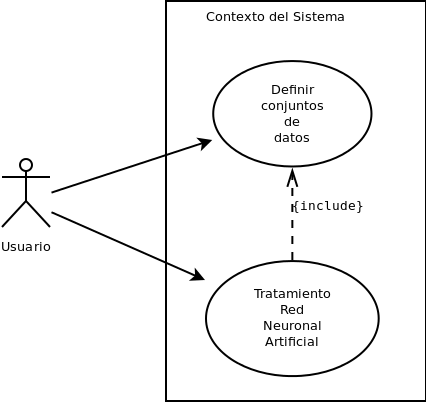
\includegraphics[scale=0.6]{uml/DiagramaContexto.png}
				\caption{Diagrama de Contexto del Sistema.}
				\label{fig:DiagramaContexto}
			\end{figure}
			
			\begin{table}[!h]
				\centering
				\begin{tabular}{l|p{.5\linewidth}}
					\hline Nombre & Contexto del Sistema. \\ 
					\hline Actores & Usuario. \\ 
					\hline Descripción & El sistema proporciona al usuario la opción de definir el conjunto de datos o de tratar la red neuronal artificial, ya sea creándola, entrenándola u obteniendo los resultados. \\ 
					\hline Casos de Uso & \textit{CU1}. \textbf{Definir el conjunto de datos}. Si el usuario quiere definir el conjunto de datos tendrá que elegir esta opción.
					
					\textit{CU2}. \textbf{Tratamiento Red Neuronal Artificial}. Si el usuario desea realizar el tratamiento de la red neuronal, ya sea crearla, entrenarla u obtener los resultados. \\ 
					\hline Flujo Principal de Eventos & El usuario comenzará eligiendo la opción que desea ejecutar, que podrá ser o definir el conjunto de datos a usar o tratar la red neuronal artificial. \\ 
					\hline 
				\end{tabular}
				\caption{Diagrama de caso de uso CU0: Contexto del Sistema.}
				\label{tab:CU0}
			\end{table}
			
			La Figura \ref{fig:CU1} y la Tabla \ref{tab:CU1} representan el caso de uso correspondiente al tratamiento de la RNA.\\
			
			\begin{figure}[!h]
				\centering
				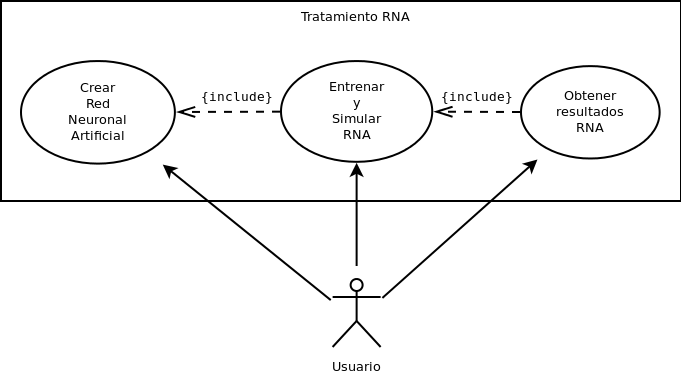
\includegraphics[scale=0.5]{uml/DiagramaNivel1.png}
				\caption{Diagrama de caso de uso CU1: Tratamiento RNA.}
				\label{fig:CU1}
			\end{figure}
			
			\begin{table}[!h]
				\centering
				\begin{tabular}{l|p{.5\linewidth}}
					\hline Nombre & Tratamiento RNA. \\ 
					\hline Actores & Usuario. \\ 
					\hline Descripción & El sistema proporciona las opciones para el tratamiento de una red neuronal artificial para regresión ordinal. \\ 
					\hline Casos de Uso & \textbf{Crear RNA}: consiste en la creación de una red neuronal artificial para regresión ordinal.
					
					\textbf{Entrenar y simular RNA}: consiste en realizar el entrenamiento de la red neuronal aplicando el algoritmo ORNNet explicado en la sección 7.1.
					
					\textbf{Obtener resultados RNA}: consiste en obtener los resultados generados por el entrenamiento y simulación del conjunto de datos en la red neuronal aplicando el algoritmo desarrollado de regresión ordinal. \\ 
					\hline Flujo Principal de Eventos & El usuario crea la red neuronal de la que, a partir de ella y del conjunto de datos cargado previamente, se realiza el entrenamiento y la simulación de la red haciendo uso del algoritmo implementado, ORNNet, del cual se obtienen los resultados para el posterior análisis de los mismos. \\ 
					\hline 
				\end{tabular}
				\caption{Diagrama de caso de uso CU1.}
				\label{tab:CU1}
			\end{table}

		\subsection{Diagrama de Secuencia}
			
			Los diagramas de Secuencia son un tipo de diagrama usados para modelar interacciones entre objetos en un sistema según UML. Un diagrama de secuencia muestra la interacción de un conjunto de objetos en una aplicación a través del tiempo y se modela para cada caso de uso. Mientras que el diagrama de casos de uso permite el modelado de una vista \textit{business} del escenario, el diagrama de secuencia contiene detalles de implementación del escenario, incluyendo los objetos y clases que se usan para implementar el escenario, y mensajes intercambiados entre los objetos.\\

			La Figura \ref{fig:secuencia} representa el diagrama de secuencia correspondiente al funcionamiento del sistema.
			
			\begin{figure}[h]
				\centering
				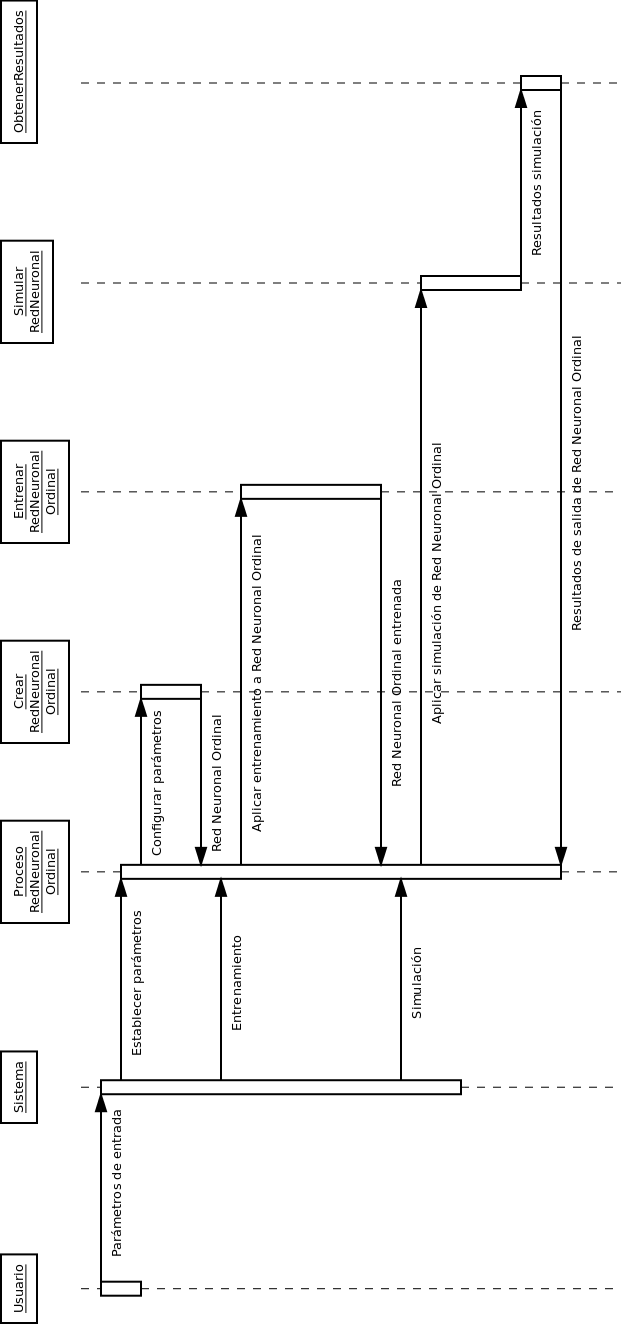
\includegraphics[scale=0.5]{uml/DiagramaSecuencia.png}
				\caption{Diagrama de Secuencia.}
				\label{fig:secuencia}
			\end{figure}

	\chapter{Diseño del sistema}
	
	En este capítulo se detallarán los módulos que serán necesarios utilizar e implementar. Para cada módulo se especificará el nombre del módulo, una descripción general del módulo, las variables que usa y las funciones que utiliza. Estos módulos se extraen tanto de los diagramas de casos de uso y de los diagramas de secuencia como de la propia definición del problema. En cada uno de los módulos que se describirán a continuación se distinguirán principalmente los siguiente apartados:
	
	\begin{itemize}
		\item \textit{Nombre del módulo:} se especificará el nombre del módulo que se vaya a explicar. Este nombre será identificativo y se corresponderá con el estilo que tiene el toolbox nnet de Matlab para que la integración sea lo más correcta posible.
		\item \textit{Descripción general del módulo:} se hará una descripción general de la funcionalidad y el manejo que tendrá el módulo.
		\item \textit{Funciones del módulo:} en el caso de que el módulo en sí no sea una función, se detallarán las funciones que se usan para el correcto funcionamiento de dicho módulo.
	\end{itemize}
	
	\section{Diseño de los módulos}
	
		En esta sección se va a realizar la especificación de los módulos que contendrá el sistema. Para ello, se hará uso de diagramas de paquetes y así poder ver la estructuración del sistema.\\
		
		En el Lenguaje Unificado de Modelado, los diagramas de Paquetes se usan para reflejar la organización de paquetes y sus elementos. Los usos más comunes de para los diagrama de paquete son para organizar diagramas de casos de uso y diagramas de clases, estos paquetes son como grandes contenedores de clases.	Los elementos contenidos en un paquete comparten el mismo espacio de nombres, esto significa que los elementos contenidos en un mismo espacio de nombres específico deben tener nombres únicos. Como otra característica de estos diagramas, cada paquete se debe identificar con un nombre único y opcionalmente mostrar todos los elementos dentro del mismo.\\
		
		Antes de realizar la especificación de cada módulo por separado, en la Figura \ref{fig:paquetes0} se muestra la estructuración general del sistema diseñado para que se ajuste lo más posible y con una estructura similar al toolbox nnet de Matlab.
		
		\begin{figure}[h]
			\centering
			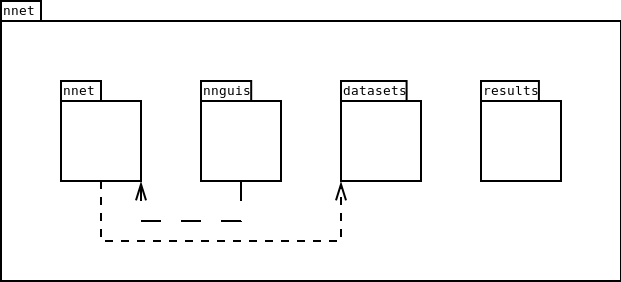
\includegraphics[scale=0.6]{uml/DiagramaPaquetes0.png}
			\caption{Diagrama de Paquetes principal}
			\label{fig:paquetes0}
		\end{figure}
		
		\subsection{Módulo principal nnet}
		
			Este será el módulo principal del sistema el cual contendrá los submódulos necesarios para el funcionamiento del sistema. Cada submódulo contendrá las funciones necesarias para la creación y tratamiento de la red neuronal artificial junto con el algoritmo propuesto en este proyecto. La organización de este módulo contiene una estructura similar al del toolbox nnet de Matlab.\\
			
			La Figura \ref{fig:paquetes1} muestra el diagrama de Paquetes para este módulo.
			
			\begin{figure}[h]
				\centering
				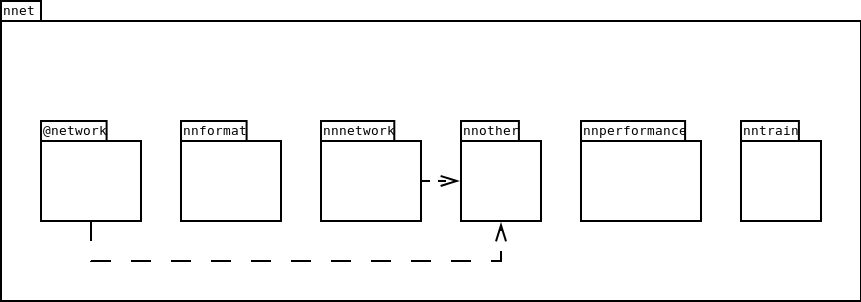
\includegraphics[scale=0.5]{uml/DiagramaPaquetes1.png}
				\caption{Diagrama de Paquetes del módulo nnet diseñado}
				\label{fig:paquetes1}
			\end{figure}
			
			La Tabla \ref{modulo_nnet} muestra la especificación breve del módulo principal.
			
			\begin{table}[!h]
				\centering
				\begin{tabular}{l|p{.5\linewidth}}
					\hline Nombre & nnet \\ 
					\hline Descripción & Módulo principal del sistema. Contendrá los principales submódulos para que el sistema funcione. \\ 
					\hline 
				\end{tabular}
				\caption{Especificación módulo nnet}
				\label{modulo_nnet}
			\end{table}
		
			\subsubsection{Módulo @network}
			
			La Tabla \ref{modulo_@network} muestra la especificación detallada del módulo así como la descripción de las funciones que contiene.
			
			\begin{table}[!h]
				\centering
				\begin{tabular}{l|p{.5\linewidth}}
					\hline Nombre & @network \\ 
					\hline Descripción & Módulo que contiene las funciones para el entrenamiento y simulación de la red neuronal pero ajustada para que los métodos se basen en la ordinalidad. \\ 
					\hline Funciones & \textit{OSIM}: función para simular una red neuronal ordinal a partir de los datos de entrada del conjunto de datos seleccionado y que devolverá las salidas obtenidas.
					
					\textit{OTRAIN}: función para entrenar una red neuronal ordinal a partir de los datos de entrada y los datos objetivo del conjunto de datos seleccionado. El entrenamiento se producirá haciendo uso del algoritmo propuesto en este proyecto, es decir, ORNnet. \\ 
					\hline 
				\end{tabular}
				\caption{Especificación módulo @network}
				\label{modulo_@network}
			\end{table}
			
			\subsubsection{Módulo nnformat}
		
			La Tabla \ref{modulo_nnformat} muestra la especificación detallada del módulo así como la descripción de las funciones que contiene.
			
			\begin{table}[!h]
				\centering
				\begin{tabular}{l|p{.5\linewidth}}
					\hline Nombre & nnformat \\ 
					\hline Descripción & Módulo que contiene la función para realizar una división estratificada de los datos. \\ 
					\hline Funciones & \textit{DIVIDESTRA}: función que realiza una división estratificada de los datos a partir de los datos objetivos los cuales son tratados para obtener un vector de elementos con identificación a la clase a la que pertenecen. \\ 
					\hline 
				\end{tabular}
				\caption{Especificación módulo nnformat}
				\label{modulo_nnformat}
			\end{table}
			
			\subsubsection{Módulo nnnetwork}
		
			La Tabla \ref{modulo_nnnetwork} muestra la especificación detallada del módulo así como la descripción de las funciones que contiene.
			
			\begin{table}[!h]
				\centering
				\begin{tabular}{l|p{.5\linewidth}}
					\hline Nombre & nnnetwork \\ 
					\hline Descripción & Módulo que contiene la función necesaria para crear una red neuronal ordinal. \\ 
					\hline Funciones & \textit{NEWOFF}: función que crea una red neuronal ordinal a partir de los datos de entrada y objetivo del conjunto de datos seleccionado, por defecto habrá al menos dos capas ocultas donde la última capa oculta tendrá solamente una neurona sin bias y se usará como función de transferencia linear. La capa de salida tendrá por defecto como función de transferencia una sigmoide logarítmica. La función de entrenamiento especificada por defecto será la de entrenamiento basado en el algoritmo modificado iRProp+ ajustado para la implementación ordinal (ORNnet). Por último, la función por defecto para análisis será la del Error Cuadrado Medio (MSE) y se utilizará una división estratificada de los datos para la simulación de la red. \\ 
					\hline 
				\end{tabular}
				\caption{Especificación módulo nnnetwork}
				\label{modulo_nnnetwork}
			\end{table}
			
			\subsubsection{Módulo nnother}
			
			La Tabla \ref{modulo_nnother} muestra la especificación detallada del módulo así como la descripción de las funciones que contiene.
			
			\begin{table}[!h]
				\centering
				\begin{tabular}{l|p{.5\linewidth}}
					\hline Nombre & nnother \\ 
					\hline Descripción & Módulo que contiene las funciones auxiliares para carga de ficheros, realización de pre o post procesamiento de los conjuntos de datos de entrada u objetivos para convertirlos o transformarlos en conjuntos de datos válidos para su posterior tratado o realización de una división estratificada. \\ 
					\hline Funciones & \textit{CONVDATA}: función que realiza, a partir del conjunto de datos de entrada y de objetivos con el formato proporcionado por NNEP de la librería del grupo AYRNA, JCLEC, la creación de los nuevos conjuntos de datos compatibles para el tratado por Matlab.
					
					\textit{CONVOUTPUTS}: función que realiza el tratado del conjunto de datos de salida proporcionado por la simulación de la red neuronal ordinal convirtiéndolo en un conjunto de datos de salida válido para su posterior procesado.
					
					\textit{GETSTRA}: función que realiza, a partir de la transformación de un conjunto de datos objetivos, la creación del vector de elementos estratificados.
					
					\textit{IMPORTFILE}: función que realiza la carga de datos de un fichero a partir del nombre del fichero.
					
					\textit{KFOLD}: función que realiza una validación de cruce haciendo un k-Fold, que por defecto será de diez folds, a partir de los datos de entrada y objetivo de la red devolviendo el número óptimo de neuronas en la capa oculta.
					
					\textit{TRANSDATA}: función que realiza la transformación de los datos objetivos para obtener como resultado un nuevo conjunto de datos objetivos compatible para el procesamiento del MSE. \\ 
					\hline 
				\end{tabular}
				\caption{Especificación módulo nnother}
				\label{modulo_nnother}
			\end{table}
			
			\subsubsection{Módulo nnperformance}
			
			La Tabla \ref{modulo_nnperformance} muestra la especificación detallada del módulo así como la descripción de las funciones que contiene.
			
			\begin{table}[!h]
				\centering
				\begin{tabular}{l|p{.5\linewidth}}
					\hline Nombre & nnperformance \\ 
					\hline Descripción & Módulo que contiene las funciones para medición del rendimiento de las salidas proporcionadas al entrenar y simular la red neuronal ordinal. \\ 
					\hline Funciones & \textit{CCRCALC}: función que realiza el cálculo del rango correctamente clasificado a partir de la matriz de confusión resultante de los datos de salida proporcionados al simular la red neuronal ordinal..
					
					\textit{MAECALC}: función que realiza el cálculo de error medio absoluto a partir de la matriz de confusión resultante de los datos de salida proporcionados al simular la red neuronal ordinal. \\ 
					\hline 
				\end{tabular}
				\caption{Especificación módulo nnperformance}
				\label{modulo_nnperformance}
			\end{table}
			
			\subsubsection{Módulo nntrain}
			
			La Tabla \ref{modulo_nntrain} muestra la especificación detallada del módulo así como la descripción de las funciones que contiene.
			
			\begin{table}[!h]
				\centering
				\begin{tabular}{l|p{.5\linewidth}}
					\hline Nombre & nntrain \\ 
					\hline Descripción & Módulo que contiene las funciones de entrenamiento para una red neuronal. Para una red neuronal ordinal se ha implementado la función de entrenamiento iRProp+ modificado con las especificaciones del algoritmo ORNnet. \\ 
					\hline Funciones & \textit{TRAINIRP}: función que realiza el entrenamiento de una red neuronal artificial aplicando el algoritmo iRProp+.
					
					\textit{TRAINIRPO}: función que realiza el entrenamiento de una red neuronal ordinal aplicando el algoritmo modificado iRProp+ con las modificación necesarias y especificadas por ORNnet. \\ 
					\hline 
				\end{tabular}
				\caption{Especificación módulo nntrain}
				\label{modulo_nntrain}
			\end{table}
			
	\section{Diseño de la interfaz}
		
		En esta sección se va a especificar cómo será el entorno que el usuario perciba al poner en funcionamiento la aplicación. Para ello se va a hacer uso de herramientas de prototipado de interfaces, concretamente de la herramienta web Balsamiq. En cada uno de los prototipos de la interfaz se especificarán cada uno de los elementos que contiene detalladamente.
		
		\subsection{Interfaz principal}
			
			La \textit{Interfaz principal} poseerá una estructura como la que se puede apreciar en la Figura \ref{fig:int0}.\\
			
			\begin{figure}[htbp]
				\centering
				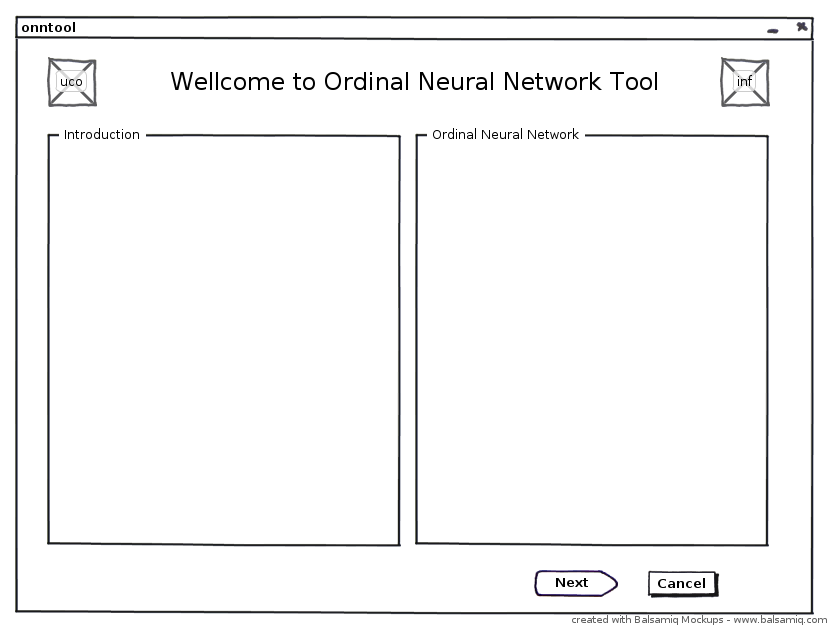
\includegraphics[scale=0.5]{interfaz/Interfaz_principal.png}
				\caption{Prototipo de la Interfaz principal}
				\label{fig:int0}
			\end{figure}
			
			La interfaz contendrá unas dimensiones de 800x600 píxeles en todo momento y, concretamente en ésta, los siguientes elementos ya sean interactivos o no:
			
			\begin{itemize}
				\item \textbf{Título:} contiene el título principal de bienvenida a la aplicación.
				\item \textbf{Imagen UCO:} imagen corporativa de la Universidad de Córdoba.
				\item \textbf{Imagen Informática:} imagen corporativa de los Ingenieros Informáticos.
				\item \textbf{Información Introducción:} cuadro que proporciona una breve información general sobre el uso de la aplicación.
				\item \textbf{Información Redes Neuronales Ordinales:} cuadro que proporciona una breve información sobre las redes neuronales artificiales ordinales.
				\item \textbf{Botón Siguiente:} botón que sirve para pasar a la siguiente interfaz.
				\item \textbf{Botón Cancelar:} botón que sirve para cerrar la interfaz en cualquier momento.
			\end{itemize}
			
			Los elementos comunes que aparezcan en las siguientes interfaces no se volverán a explicar para que no exista redundancia de información.
		
		\subsection{Interfaz de datos}
		
			La \textit{Interfaz de datos} poseerá una estructura como la que se puede apreciar en la Figura \ref{fig:int1}.\\
			
			\begin{figure}[htbp]
				\centering
				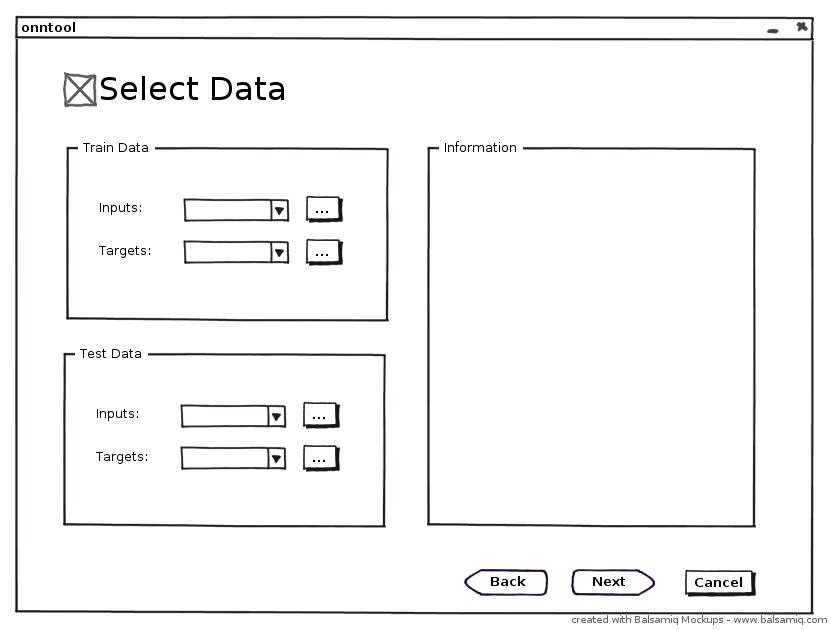
\includegraphics[scale=0.5]{interfaz/Interfaz_datos.png}
				\caption{Prototipo de la Interfaz de datos}
				\label{fig:int1}
			\end{figure}
			
			La interfaz contendrá los siguientes elementos, ya sean interactivos o no:
			
			\begin{itemize}
				\item \textbf{Título:} contiene el título representativo de la interfaz.
				\item \textbf{Botón de selección de datos de entrada (train y test):} botón que muestra la información del conjunto de datos de entrada.
				\item \textbf{Botón de selección de datos objetivos (train y test):} botón que muestra la información del conjunto de datos objetivos.
				\item \textbf{Botones de selección de datos (train y test):} botón que, a partir de una interfaz de carga de datos, selecciona un fichero externo y carga los datos para tratarlos.
				\item \textbf{Información de ayuda:} cuadro que proporciona una breve información de la interfaz.
				\item \textbf{Botón Atrás:} botón que sirve para pasar a la interfaz anterior.
			\end{itemize}
			
		\subsection{Interfaz para la creación de la red neuronal}
		
			La \textit{Interfaz de red neuronal} poseerá una estructura como la que se puede apreciar en la Figura \ref{fig:int2}.\\
			
			\begin{figure}[htbp]
				\centering
				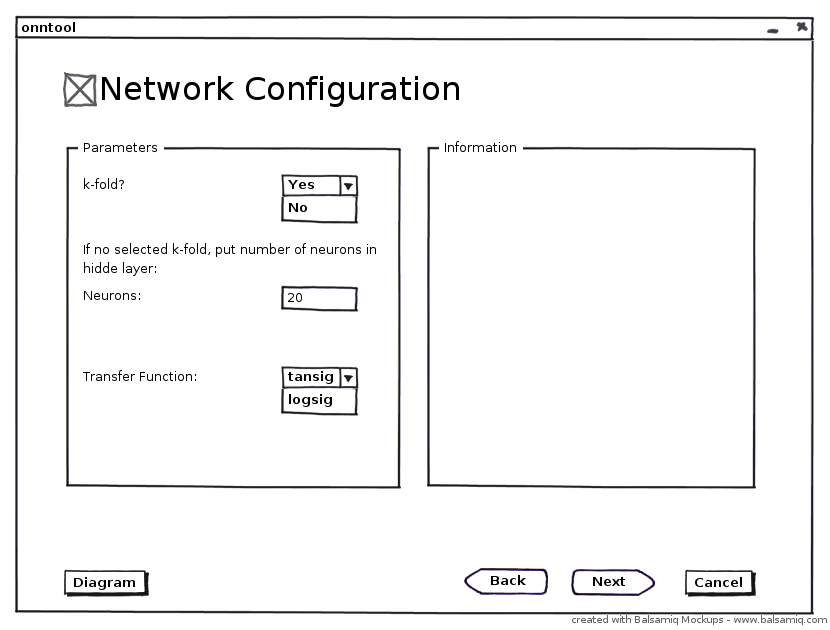
\includegraphics[scale=0.5]{interfaz/Interfaz_net.png}
				\caption{Prototipo de la Interfaz de red neuronal}
				\label{fig:int2}
			\end{figure}
			
			La interfaz contendrá los siguientes elementos, ya sean interactivos o no:
			
			\begin{itemize}
				\item \textbf{Opción de realización de k-fold:} botón que da la opción de realizar un k-fold para los conjuntos de datos.
				\item \textbf{Número de neuronas:} en caso de no activar la opción de k-fold se podrá especificar el número de neuronas que tendrá la capa oculta.
				\item \textbf{Opción para la función de transferencia:} al igual que el anterior, cuando no esté activa la opción del k-fold, se tendrá que especificar la función de transferencia.
				\item \textbf{Botón de Diagrama:} botón que da la posibilidad de mostrar de forma gráfica como se organiza la red neuronal artificial ordinal.
			\end{itemize}
			
		\subsection{Interfaz de entrenamiento y simulación}
		
			La \textit{Interfaz de entrenamiento y simulación} poseerá una estructura como la que se puede apreciar en la Figura \ref{fig:int3}.\\
			
			\begin{figure}[htbp]
				\centering
				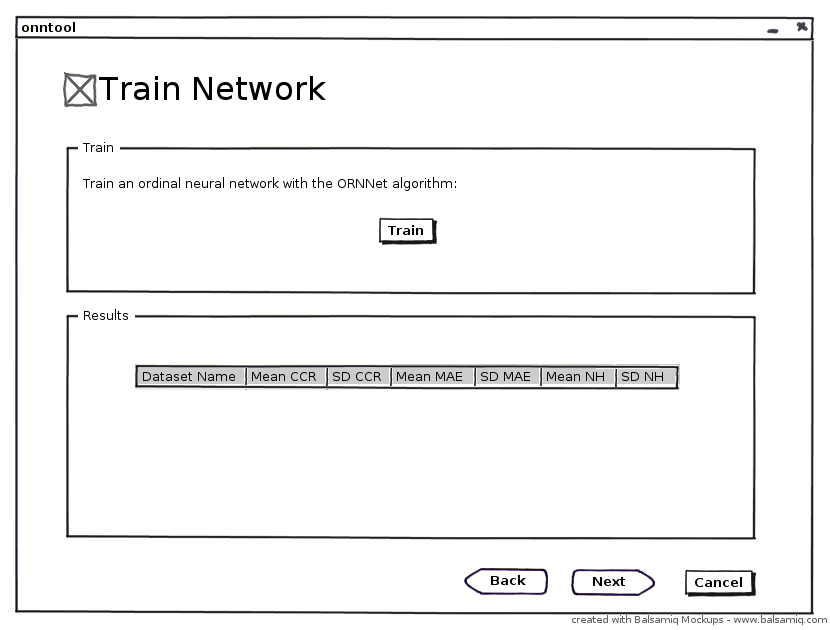
\includegraphics[scale=0.5]{interfaz/Interfaz_train.png}
				\caption{Prototipo de la Interfaz de entrenamiento}
				\label{fig:int3}
			\end{figure}
			
			La interfaz contendrá los siguientes elementos, ya sean interactivos o no:
			
			\begin{itemize}
				\item \textbf{Botón de entrenamiento:} botón que entrena y simula la red neuronal a partir de los datos de entrenamiento y test del conjunto de datos.
				\item \textbf{Resultados:} muestra los resultados obtenidos a partir de la simulación.
			\end{itemize}
		
		\subsection{Interfaz de exportación de datos}
		
			La \textit{Interfaz de exportación} poseerá una estructura como la que se puede apreciar en la Figura \ref{fig:int4}.\\
			
			\begin{figure}[htbp]
				\centering
				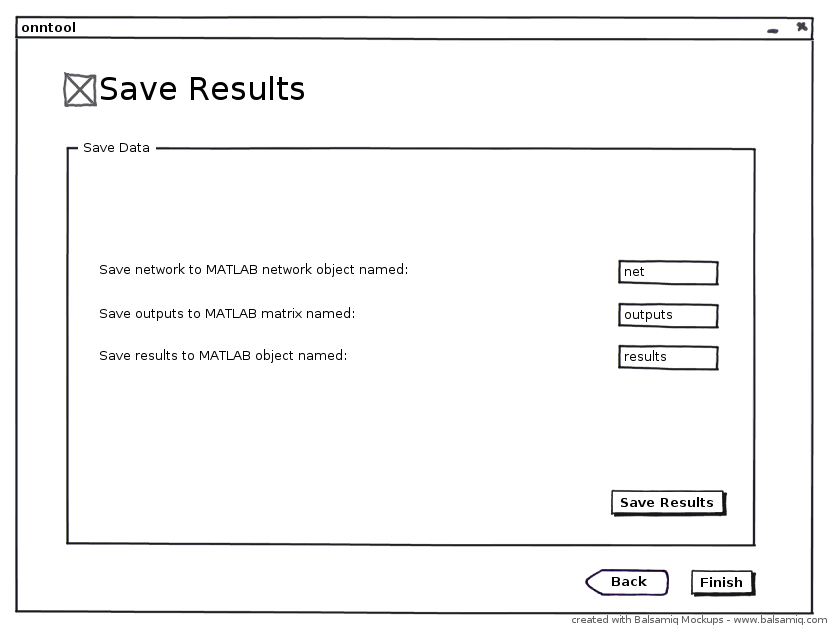
\includegraphics[scale=0.5]{interfaz/Interfaz_export.png}
				\caption{Prototipo de la Interfaz de exportación}
				\label{fig:int4}
			\end{figure}
			
			La interfaz contendrá los siguientes elementos, ya sean interactivos o no:
			
			\begin{itemize}
				\item \textbf{Nombre para guardar la red neuronal:} campo para especificar como se llamará la variable que almacenará la estructura de la red neuronal.
				\item \textbf{Nombre para guardar las salidas obtenidas:} campo para especificar como se llamará la variable que almacenará la matriz de salida.
				\item \textbf{Nombre para guardar los resultados de salida (CCR, MAE, NH):} campo para especificar como se llamará la variable que almacenará la matriz de resultados.
				\item \textbf{Botón Guardar Resultados:} botón que guardará los resultados en el espacio de trabajo de Matlab.
				\item \textbf{Botón Finalizar:} botón que cerrará la interfaz al dar el proceso por finalizado.
			\end{itemize}

	\chapter{Implementación}
	
	En este capítulo se detallarán aquellas particularidades para la implementación real del algoritmo de regresión ordinal y las redes neuronales. Para ello, se han seguido los manuales y tutoriales, además de las guías de referencia que el propio Matlab proporciona \cite{Matlab_ref,Matlab_nnet,Matlab_gui}.
	
	\section{Entrenamiento y Simulación}
	
		\textbf{Función osim}\\
		
		Esta función tiene como particularidades que hay que hacer un tratamiento de las salidas después de simular la red neuronal ordinal, es decir, hay que poner la última línea de resultados a 1 para que la probabilidad acumulada sea correcta en todos los casos alcanzando este valor. Después de este tratamiento, se hace uso de la función \textit{convoutputs} la cual realiza una conversión de las salidas para que se convierta de una salida con probabilidades acumuladas a una salida con resultados binarios, donde se pondrá un 1 cuando sea la clase con mayor probabilidad y un 0 en el resto.\\
		
		Se muestra el código parcial para que quede clara la implementación.\\
		
		\lstinputlisting[firstline=29, lastline=37, caption={Archivo osim.m}]{../src/nnet/@network/osim.m}
		
		\textbf{Función otrain}\\
		
		Esta función tiene como particularidad la llamada ajustada a la función de entrenamiento que se ha implementado en este proyecto y que posteriormente se mostrará con sus particularidades. Esta llamada se encuentra ajustada ya que los valores objetivos de la última entrada no hace falta tratarlos cuando se trate de una red neuronal ordinal.\\
		
		\lstinputlisting[firstline=31, lastline=32, caption={Archivo otrain.m}]{../src/nnet/@network/otrain.m}
		
	\section{Entrenamiento ordinal}
		
		\textbf{Función trainirpo}\\
		
		Esta función tiene las mayores peculiaridades en comparación con el resto, ya que es la que aplica la actualización y ajuste del algoritmo iRProp+ para redes neuronales ordinales. En la línea 15 se muestra el tratado especial que hay que tener para que las bias se analicen en un paso posterior y que los pesos no se modifiquen. A partir de la línea 21 se hace el nuevo procesado de los sesgos o \textit{bias}, ya que en este caso, las \textit{bias} hay que tratarlas para que se mantenga la condición, $b_1 < b_2 < \cdots < b_J-1$.\\
		
		\lstinputlisting[firstline=322, lastline=360, caption={Archivo trainirpo.m}]{../src/nnet/nntrain/trainirpo.m}
		
	\section{Creación de una red neuronal ordinal}
	
		\textbf{Función newoff}\\
		
		Esta función tiene bastantes peculiaridades ya que es de las más importantes al crear e inicializar la red neuronal artificial de forma ordinal. Desde la línea 3 hasta la 23 se muestra como, a partir de los parámetros de entrada, se crea la red neuronal con los parámetro ajustados y fijos necesarios para que se realice el proceso para una red neuronal ordinal. Entre los ajustes que se realizan, se pueden observar que las dos últimas capas son fijas, las funciones de transferencia para esas capas también lo son. Además, la función de entrenamiento es la comentada anteriormente y la función para la división inicial de los datos es una división estratificada y no la que vendría por defecto.\\
		
		Las líneas a partir de la 25 serían los ajustes posteriores a la creación de la red neuronal y que no se pueden establecer en el momento de la creación de la misma. Entre otros, se determina los pesos fijos que debe tener la última capa, la eliminación del sesgo intermedio, la inicialización de los \textit{bias} para que cumplan la condición que antes se ha comentado y los porcentajes de cada uno de los patrones para los conjuntos de entrenamiento, test y validación.\\
		
		\lstinputlisting[firstline=64, lastline=102, caption={Archivo newoff.m}]{../src/nnet/nnnetwork/newoff.m}
		
	\section{Cálculo del número óptimo de neuronas en la capa oculta}
		
		\textbf{Función kfoldo}\\
		
		Esta función tiene como peculiaridad la potencia que Matlab tiene para realizar cálculos y procesamiento de grandes operaciones computacionales. Para comenzar, se realiza una llamada a una de las funciones implementadas la cual obtiene las clases para un conjunto de datos, en la línea 3. Seguidamente, la función \textit{crossvalind} obtiene los índices de una forma semialeatoria realizando un K-Fold\footnote{Método explicado en el capítulo de Experimentación.}. A partir de esos índices, se definen los nuevos conjuntos de datos de entrenamiento y, de este modo, realizar, un número determinado de veces, la creación, entrenamiento y simulación de la red neuronal para posteriormente obtener los datos de las salidas y poder calcular la matriz de confusión. A partir de la matriz de confusión y realizando la media del número determinado de ejecuciones del mismo, se obtendrá el \textit{MAE}. Para determinar el número de neuronas en capa oculta se seleccionará aquel número que conforme modelos que proporcionan un menor \textit{MAE}.\\
		
		\lstinputlisting[firstline=38, caption={Archivo kfoldo.m}]{../src/nnet/nnother/kfoldo.m}

	\chapter{Pruebas}

	La fase de pruebas es una parte fundamental en el desarrollo de cualquier sistema ya que determinará la calidad del mismo. A lo largo del desarrollo del sistema se realizan un conjunto de controles que determina de esta forma la calidad del mismo y para poder detectar errores cuanto antes, ya que a medida que el desarrollo avanza, cualquier corrección del sistema puede ser mucho más costosa de solucionar tanto en tiempo como en esfuerzo.\\
	
	Si se considera el sistema como un conjunto de componentes que interactúan entre sí, esto da lugar a la necesidad de probar estos componentes por separado para demostrar que cada uno de ellos funciona correctamente y que produce unos resultados satisfactorios, de esta forma es necesario incluir pruebas de los componentes antes de realizar las pruebas de todo el conjunto.\\
	
	Con muchas de estas pruebas no sólo se busca un correcto funcionamiento, sino también óptimo, ya que es necesario el entrenamiento de diferentes parámetros que con determinados valores pueden dar resultados buenos pero inferiores al máximo esperado, de esta forma es necesario realizar pruebas que permitan optimizar los valores de entrada del sistema.\\
	
	Se va a mostrar una introducción teórica sobre el fundamento y finalidad de las pruebas y a continuación el catálogo de pruebas.\\
	
	Las características fundamentales de las pruebas se pueden resumir en los siguientes puntos:
	
	\begin{enumerate}
		\item La prueba es un proceso de ejecución de un programa con la intención de descubrir un error.
		\item Un buen caso de prueba es aquel que tiene una alta probabilidad de mostrar un error no descubierto hasta entonces.
		\item La filosofía más adecuada para las pruebas consiste en planificarlas y diseñarlas de la forma más sistemática posible para poder detectar el máximo número y variedad de defectos con el mínimo consumo de tiempo y esfuerzo.
	\end{enumerate}

	\section{Estrategia de pruebas}
	
		Hay que intentar diseñar un conjunto de casos de prueba que permita conseguir una confianza aceptable que encuentre los defectos existentes y a la vez que los resultados obtenidos seas lo suficientemente buenos con respecto a un margen establecido teniendo que optimizar en caso contrario.\\
		
		Como entorno de pruebas para este sistema se han desarrollado una serie de pruebas denominadas \textit{pruebas de caja negra} y \textit{pruebas de caja blanca}. Los resultados de estas pruebas han llevado a la detección de errores que se han ido solucionando volviendo a fases anteriores y volviendo a realizar seguidamente las pruebas hasta obtener un resultado satisfactorio.\\
		
		El procedimiento utilizado para eliminar errores es, por tanto, la \textit{vuelta atrás}, localizando el síntoma que indujo a pensar que había un error e ir hacia atrás hasta llegar a la causa del mismo. A su vez, el conjunto de casos de prueba realizados se pueden clasificar en 4 tipos que se irán explicando en las siguientes subsecciones.
		
		\subsection{Pruebas Unitarias}

			El conjunto de pruebas que forman esta parte se trata de un conjunto de pruebas unitarias de los componentes del sistema y, por lo tanto, la verificación de la menor unidad del diseño del software, el módulo. Se considera como módulo a un bloque básico de construcción de programas, una parte del código que implementa una función simple o un fragmento de código que se puede compilar y/o probar independientemente. Normalmente tienen una longitud menor de 500 líneas de código. Éste se compone de dos tipos de pruebas, como se ha comentado anteriormente, pruebas estructurales o \textit{pruebas de caja blanca} y pruebas funcionales o \textit{pruebas de caja negra}.\\
			
			Las pruebas de caja blanca están relacionadas con la fase de diseño, así, se intenta mostrar la validación de los componentes que conforman el sistema por lo que es necesario probar la funcionalidad de cada uno de los componentes por separado demostrando que cumplen con su tarea de forma óptima y no causan ningún error.\\
			
			Básicamente, se intenta probar cada una de las líneas de código que conforman el sistema, normalmente las combinaciones que se pueden llevar a cabo de la ejecución del sistema son muy numerosas debido a la existencia de bucles, sentencias condicionales, etc. Sin embargo, es necesario probar que cada una de esas sentencias realiza una acción de forma correcta, es decir, será necesario realizar una cobertura de sentencias que demuestre que ese trozo de código se ejecuta correctamente.\\
			
			Los resultados de estas pruebas han llevado a la detección de errores solucionados en la fase de codificación, buscando la causa a partir de los síntomas que delataban el error y de este modo, realizando las oportunas acciones para corregirlos.\\
			
			De esta forma y a medida que se iban implementando las distintas funciones y módulos de ejecución del sistema, se iba comprobando su eficiencia y estructura para comprobar que no se producía ningún tipo de error.\\
			
			Estas pruebas se han realizado de la siguiente forma:
			
			\begin{enumerate}
				\item Se ha comprobado, para cada módulo, si se almacenaba y trataba correctamente toda la información contenida en las estructuras internas de datos.
				\item Se ha comprobado que el flujo de información se realiza correctamente para todas las ramas posibles del módulo.
				\item Se han realizado pruebas en los límites de los bucles.
				\item Se ha comprobado la ejecución de cada una de las sentencias que forman parte del módulo, analizando la ejecución completa de cada módulo.
			\end{enumerate}
			
			Las pruebas de caja negra se han desarrollado de forma paralela y posterior a la composición de todos los componentes que forman parte del sistema. Dichas pruebas se centran en las acciones visibles al usuario y salidas reconocibles desde el sistema en lo que se espera de un módulo. Por ello, se denominan pruebas funcionales, limitándose a suministrar datos como entrada y estudiar la salida sin preocuparse de lo que pueda estar haciendo el módulo por dentro.\\
			
			Las pruebas de caja negra se apoyan en la especificación del sistema. Así, para cada módulo:
			
			\begin{enumerate}
				\item Se ha realizado un estudio de los posibles valores correctos en los parámetros de tipo dato, centrándose en las condiciones límite.
				\item Se ha analizado qué valores se esperaban como resultado del módulo y en qué condiciones habían de darse, se proporcionaron datos de entrada a los algoritmos y se comprobó que la salida era la esperada.
				\item Para realizar todas estas pruebas se han utilizado pequeños programas de prueba en los que se cargaban las funciones o los módulos con los valores necesarios para cubrir el caso de prueba a realizar, se realizaba el método y se mostraban los resultados.
			\end{enumerate}
		
		\subsection{Pruebas de Integración}

			De igual modo, para comprobar que la estructura del sistema y el control del mismo se ejecutan de forma correcta, es necesario llevar a cabo un conjunto de pruebas de integración que permitan comprobar que el flujo de datos entre módulos es correcto.\\
			
			Pruebas integrales o pruebas de integración son aquellas que se realizan en el ámbito del desarrollo del software una vez que se han aprobado las pruebas unitarias de dichos módulos. Únicamente se refieren a la prueba o pruebas de todos los elementos unitarios que componen un proceso hecha en conjunto.\\
			
			Las pruebas de integración se han realizado de forma ascendente, es decir, se trata mediante un proceso incremental en el cual se comprueba el siguiente módulo con el conjunto de módulos que ya han sido probados, este proceso continua hasta llegar a probar el sistema completo. De esta forma se comienza por los módulos de más bajo nivel hasta alcanzar el sistema al completo.\\
			
			De este modo, estas pruebas se han realizado de la siguiente forma:
			
			\begin{enumerate}
				\item Se ha comprobado en cada paso incremental que la interacción entre el módulo añadido con el conjunto de módulos ya probados funciona correctamente.
				\item Se ha comprobado que el flujo de información se realiza correctamente entre los diferentes módulos.
				\item Se ha comprobado que la ejecución de todas las ramas posibles del conjunto de módulos del sistema hasta que el punto alcanzado sea correcto.
			\end{enumerate}
			
			Otro apartado importante a puntualizar es la integración del sistema en Matlab como parte del toolbox nnet, así, fue necesario realizar una serie de pruebas que demostraran que el sistema podría funcionar perfectamente en concordancia con el toolbox original, administrando los valores de entrada dados por éste y proporcionándole posteriormente los resultados como valores de salida.
		
		\subsection{Pruebas del Sistema}
		
			Tras la finalización de las pruebas anteriores se obtendrá un sistema completo funcionalmente correcto y del que han sido solventados todos los posibles errores que hayan ido surgiendo gracias a dichas pruebas, por lo que se puede comenzar una serie final de pruebas del software para verificar que se han integrado adecuadamente todos los elementos del sistema y que se realizan las funciones apropiadas.\\
			
			La fase de pruebas del sistema tiene como objetivo verificar el sistema software para comprobar si éste cumple los requisitos. Dentro de esta fase se pueden desarrollar varios tipos distintos de pruebas en función de los objetivos. Algunos tipos son, pruebas funcionales, pruebas de usabilidad, pruebas de rendimiento, pruebas de seguridad, etc.\\
			
			También se ha tenido muy en cuenta la velocidad de ejecución de los algoritmos desarrollados, ya que en este tipo de sistemas característicos por una aplicación iterativa de cálculos, pequeños detalles de implementación pueden influir fuertemente en el rendimiento final. Se ha preferido una mayor velocidad de cómputo  frente a la restricción del consumo de memoria. A pesar de esto, se ha realizado un control del consumo de recursos del sistema aunque no muy exhaustivo.\\
			
			En este proyecto, estas pruebas se realizarán durante las pruebas de experimentación que se pueden encontrar en el siguiente capítulo. De esta forma, se cumple con el doble objetivo de ejercitar a fondo el sistema cumpliendo con las pruebas del sistema y de comprobar si la utilización de los modelos teóricos propuestos ha merecido la pena en comparación con los resultados de los que se dispone en otros medios.
		
		\subsection{Pruebas de Aceptación}
		
			Estas pruebas las realiza el usuario final. Son básicamente pruebas funcionales sobre el sistema completado y buscan una cobertura de la especificación del sistema. Estas pruebas no se realizan durante el desarrollo pues no tendría mucho sentido de cara al usuario, sino una vez pasadas todas las pruebas de integración.\\
			
			La experiencia muestra que aun después del más cuidadoso proceso de pruebas por parte del desarrollador quedan una serie de errores que sólo aparecen cuando el usuario se pone a usarlo.\\
			
			Este tipo de pruebas se han desarrollado de dos formas, las primeras pruebas del proceso consisten en invitar al usuario a que venga al entorno de desarrollo a probar el sistema. Se trabaja en un entorno controlado y el usuario tiene siempre a un experto a mano para ayudarle a usar el sistema y para analizar los resultados.\\
			
			Las siguiente pruebas se desarrollan en el entorno del usuario, buscando un entorno que esté fuera del control. Ahí, el usuario se queda a solas con el sistema y trata de encontrarle fallos (reales o en su opinión) de los que informa al desarrollador. En este proceso, el usuario es el único con posibilidad de encontrar cualquier error que se le haya pasado al desarrollador o de buscar una mayor comodidad o eficiencia del sistema, éste es un proceso que puede llevar semanas o incluso meses dependiendo de la complejidad del sistema y del usuario final.

	\chapter{Experimentación}
	
	El capítulo de experimentación tiene como finalidad dar una idea de las estrategias seguidas en el desarrollo del software y de los resultados obtenidos en las mismas. El proceso de experimentación consiste en someter al software a una evaluación para comprobar que se comporta de acuerdo a las especificaciones y poder obtener conclusiones de su ejecución y sus resultados. La información obtenida en la experimentación ayudará a definir los parámetros idóneos para el algoritmo y de este modo mejorar su ejecución.
	
	\section{Configuración software y hardware}
	
		En esta sección se detalla la configuración software y hardware de la máquina donde se ejecutará la experimentación:\\
		
		\textbf{Software}
		
		\begin{itemize}
			\item Sistema Operativo Ubuntu Server 10.04.2 LTS.
			\item Matlab Version 7.8.0.347 (R2009a).
		\end{itemize}
		
		\textbf{Hardware}
		
		\begin{itemize}
			\item Microprocesadores Intel Xeon E5405 2.00GHz.
			\item Memoria RAM 8 GB.
		\end{itemize}
	
	\section{Condiciones de los experimentos}
	
		La aplicación de los experimentos se ha realizado de manera sistemática, procurando encontrar siempre los valores óptimos de los parámetros de configuración para resolver de la mejor forma posible los diversos problemas que puedan surgir. Para poder llevar a cabo dichos experimentos, es necesario establecer el diseño experimental de los mismo y utilizar un conjunto de bases de datos reales que permitan llevar a cabo las pruebas.\\
	
		\subsection{Diseño experimental}
		
			Para la cálculo del número de neuronas óptimo en la capa oculta se utilizará:
			
			\begin{description}
				\item[k-fold:] Proceso de validación cruzada en el que el conjunto de datos se divide al azar en \textit{k} conjuntos de datos. De esos \textit{k} conjuntos de datos, uno es utilizado como datos de validación para testear el modelo, mientras que las restantes se usan como datos de entrenamiento. El proceso de validación cruzada es, entonces, repetido \textit{k} veces, usando cada vez un conjunto de datos diferente para cada validación. Los \textit{k} resultados obtenidos se combinan luego (normalmente mediante el cálculo de la media de la medida de rendimiento utilizada) para obtener una única estimación.
			\end{description}
			
			Una vez obtenidos los resultados, se realiza un análisis indicando si concuerdan con los esperados e incluso si han superado las expectativas o el margen de error que se producido es menor. Para valorar los modelos obtenidos se utilizará, el ratio de patrones correctamente clasificados (CCR) y el error absoluto medio (MAE), explicados con anterioridad en el capítulo de Antecedentes.
	
	\section{Conjuntos de datos}
		
		Se ha llevado a cabo experimentos sobre 20 conjuntos de datos de dominio público. Estos conjuntos de datos presentan una buena diversidad respecto a diferentes características.\\
		
		Los conjuntos de datos se obtendrán de los proporcionados por el grupo de investigación, éstos se encontrarán divididos mediante un Hold-out en dos, un subconjunto de entrenamiento y otro de test, siendo el de entrenamiento mayor que el de test, aproximadamente un 75\% por ciento para entrenamiento y un 25\%.\\
		
		En la Tabla \ref{tab:datasets} se detallan las características de los conjuntos de datos empleados. Los atributos que se mostrarán en la tabla son, el nombre del conjunto de datos, número total de patrones de entrenamiento, el número total de patrones de test, el número de atributos y número de clases.\\
		
		\begin{table}[!h]
				\centering
				\begin{tabular}{l|c|c|c|c}
					\hline \textbf{Nombre} & \textbf{N.T.P. Entrenamiento} & \textbf{N.T.P. Test} & \textbf{Núm. Atributos} & \textbf{Núm. Clases} \\ 
					\hline Automobile & 1530 & 520 & 71 & 6 \\ 
					\hline Balance Scale & 4680 & 1570 & 4 & 3 \\ 
					\hline Bondrate & 420 & 150 & 37 & 5 \\ 
					\hline Car & 12960 & 4320 & 21 & 4 \\ 
					\hline Contact Lenses & 180 & 60 & 6 & 3 \\ 
					\hline Depression & 1010 & 1320 & 7 & 3 \\ 
					\hline ERA & 7500 & 2500 & 4 & 9 \\ 
					\hline ESL & 3660 & 1220 & 4 & 9 \\ 
					\hline Eucalyptus & 5520 & 1840 & 91 & 5 \\ 
					\hline LEV & 7500 & 2500 & 4 & 5 \\ 
					\hline New Thyroid & 1610 & 540 & 5 & 3 \\ 
					\hline Pasture & 270 & 90 & 25 & 3 \\ 
					\hline Squash Stored & 390 & 130 & 51 & 3 \\ 
					\hline Squash Unstored & 390 & 130 & 52 & 3 \\ 
					\hline SWD & 7500 & 2500 & 10 & 4 \\ 
					\hline TAE & 1130 & 380 & 54 & 3 \\ 
					\hline Thyroid & 54000 & 18000 & 21 & 3 \\ 
					\hline Winequality Red & 11990 & 4000 & 11 & 6 \\ 
					\hline Winequality White & 36730 & 12250 & 11 & 7 \\ 
					\hline 
				\end{tabular}
				\caption{Conjuntos de datos usados.}
				\label{tab:datasets}
			\end{table}
			
			A continuación se hará una descripción de cada uno de los conjuntos de datos:
			
			\begin{itemize}
				\item \textit{Automobile}: este conjunto de datos consiste en tres tipos de entidades: 1) la especificación de una automóvil en términos de varias características. 2) su clasificación de riesgo asignado inseguro, 3) sus pérdidas normalizadas en uso en comparación con otros coches. La segunda clasificación corresponde con el grado en el cual un automóvil tiene más riesgo del que su precio indica. Entonces, si es más arriesgado (o menos), ésto se ajusta por el movimiento hacia arriba (o hacia abajo) de la escala. A este proceso lo suelen llamar "simboling".\\

El tercer factor es el pago relativo medio de pérdida por vehículos inseguros por año. Este valor está normalizado para todos los automóviles sin un tamaño particular en la clasificación (pequeño de dos puertas, furgonetas, deportivos, etc.) y representa la media de pérdidas por coche por año.
				\item \textit{Balance Scale}: este conjunto de datos se generó a partir de los resultados de un modelo experimental psicológico. Cada ejemplo se clasifica como la punta de la balanza a la derecha, a la izquierda o balanceado. Los atributos son el peso de la punta izquierda, el de la derecha y la distancia correcta. El camino correcto para encontrar la clase es el mayor entre (distancia izquierda * peso izquierda) y (distancia derecha * peso derecha). Si son iguales, se encuentra balanceada.
				\item \textit{Bondrate}: conjunto de datos basado en el rango de bondad que existe en datos de varias ciudades a partir de datos como el número de personas residentes, el rango de ingresos entrantes, etc.
				\item \textit{Car}: el conjunto de datos de evaluación de coches se derivó desde un modelo simple de decisión jerárquico. Debido a la estructura conocida, este conjunto de datos puede ser particularmente útil para testeo de inducción constructiva y métodos de descubrimiento de estructuras.
				\item \textit{Contact Lenses}: este conjunto de datos contiene 3 tipos de clases, la primera clase se refiere al paciente que debería llevar unas lentes de contacto duras, la segunda clase se refiere al paciente que debería de llevar unas lentes de contacto blandas y por último, la tercera clase sería que el paciente no debe de llevar lentes de contacto.
				\item \textit{Depression}: conjunto de datos que contiene 3 tipos de clases, unidad espacial con depresión, unidad espacial sin depresión y unidad espacial donde no hay depresión. Este conjunto de datos proviene de casos reales obtenidos en Andalucía, al sur de España.
				\item \textit{ERA}: el ECMWF ERA-40 Re-Analysis Project consiste en un número de conjuntos de datos climáticos que abarcan el periodo entre mediados de 1957 a agosto de 2002 usando un modelo consistente.
				\item \textit{ESL}: el conjunto de datos ESL (Employee Selection) contiene perfiles de solicitantes de ciertos puestos de trabajo industriales. Expertos psicólogos de una compañía de reclutamiento, basándose en resultados de test psicométricos y entrevistas con los candidatos, determinaron los valores de los atributos de entrada. La salida es la clasificación general correspondiente a los grados de aptitud del candidato para ese tipo de trabajo.
				\item \textit{Eucalyptus}: este conjunto de datos tiene como objetivo determinar qué lotes de semillas son mejores para la conservación del suelo en una región montañosa y en una estación seca. La determinación de ésto se haya mediante la medición de parámetros como la medición de la altura, diámetro por altura, supervivencia y otros factores contribuyentes.
				\item \textit{LEV}: conjunto de datos que se usa para entrenamiento y simulación de redes neuronales.
				\item \textit{New Thyroid}: este conjunto de datos esta reducido a partir de otro y provee resultados de clasificación del funcionamiento normal, hipoactivo o hiperactivo de la glándula tiroides en base a 5 atributos.
				\item \textit{Pasture}: el conjunto de datos de producción de pastos tiene como objetivo predecir la producción de pasto mediante una variedad de factores biofísicos. Las variables de vegetación y suelo de las zonas de pastoreo de North Island, país montañoso el cual tiene diversas aplicaciones tales como aplicación de fertilizantes o paso con animales de carga.
				\item \textit{Squash Stored}: este conjunto de datos tiene como objetivos determinar qué variables antes de la cosecha dan un buen sabor a la calabaza después de diversos periodos de tiempo almacenada. Esto se determina mediante una medida de aceptabilidad categorizada como aceptable, no aceptable o excelente.
				\item \textit{Squash Unstored}: este conjunto de datos tiene como objetivos los mismo que el conjunto de datos anterior, la única diferencia es que en éste, el fruto no se almacena antes de medirse, por lo que carece de uno de los atributos, el peso de la fruta después de su almacenaje. 
				\item \textit{SWD}: el conjunto de datos Social Workers Decisions (Ordinal SWD) contiene las evaluaciones del mundo real de trabajadores sociales cualificados en relación con el riesgo al que se enfrentan los niños si ellos se quedasen con sus familias en sus casas. Esta valoración de la evaluación de riesgos es, a menudo, presentada a las cortes judiciales para ayudar a decidir que es lo mejor para un niño que presuntamente padece abusos o está descuidado.
				\item \textit{TAE}: el conjunto de datos Teaching Assistant Evaluation consiste en evaluaciones del desempeño docente sobre tres semestres regulares y dos semestres de verano de asistencia educacional asignada al Departamento de Estadística de la Universidad de Wisconsin (Madison). Las puntuaciones se dividieron en tres categorías de iguales tamaños (bajo (1), medio (2), alto (3)) para formar la variable de clases.
				\item \textit{Thyroid}: este conjunto de datos es uno de las variadas bases de datos sobre Tiroides disponible en el repositorio de la UCI. La tarea que tiene es detectar si un paciente dado es normal (1) o sufre de hipertiroidismo (2) o de hipotiroidismo (3).
				\item \textit{Winequality Red}: este conjunto de datos se encuentra relacionado a la variante roja del vino de Portuguese Vinho Verde. Debido a los problemas de privacidad y logística, solo las variables físico-químicas (entradas) y sensoriales (salidas) están disponibles. Este conjunto de datos se puede usar para tareas tanto de clasificación como de regresión. Las clases están ordenadas y no balanceadas.
				\item \textit{Winequality White}: este conjunto de datos se encuentra relacionado a la variante blanca del vino de Portuguese Vinho Verde. Debido a los problemas de privacidad y logística, solo las variables físico-químicas (entradas) y sensoriales (salidas) están disponibles. Este conjunto de datos se puede usar para tareas tanto de clasificación como de regresión. Las clases están ordenadas y no balanceadas.
			\end{itemize}
			
			El aprendizaje a partir de datos no balanceados, como son algunos de los conjuntos de datos utilizados, puede resultar dificultoso. Se dice que un conjunto de datos se encuentra no balanceado cuando presenta una desigualdad marcada en la distribución de las clases, es decir, que hay diferencias acusadas entre el número de ejemplos de las distintas clases. El problema surge porque, normalmente, los algoritmos de aprendizaje y clasificación en computación genética o evolutiva o mediante redes neuronales, que se usan para construir los clasificadores, tienden a centrarse en las clases mayoritarias y a pasar por alto las minoritarias. La consecuencia directa de este comportamiento es que el clasificador no será capaz de clasificar correctamente los ejemplos correspondientes a las clases menos frecuentes.\\
			
			La estrategia de aprendizaje no es la única cuestión que hay que afrontar cuando se trabaja con datos no balanceados. Otro punto fundamental es el de cómo medir la calidad de los clasificadores obtenidos. En clasificación, el rendimiento se suele medir en términos de la tasa de aciertos, es decir, la proporción de ejemplos correctamente clasificados o en términos de errores, ya sean medios o absolutos. \\
			
			El tamaño del conjunto de datos es hasta el momento el factor más relevante que limita la resolución de problemas de clasificación mediante este tipo de métodos debido a que el tiempo computacional requerido para clasificar grandes conjuntos de datos es excesivamente alto.
		
	\chapter{Resultados}
	
	En este capítulo se detallarán los resultados de las ejecuciones del sistema con el objetivo de analizar los resultados y de este modo, obtener conclusiones que apoyen los objetivos del proyecto.
	
	\section{Resultados individuales}
		
		En esta sección se presentarán los resultados individuales generados por cada conjunto de datos al aplicar el algoritmo realizado para el entrenamiento y simulación de las redes neuronales artificiales ya sea de forma ordinal o nominal.\\
		
		Para la obtención de los datos se ha realizado un 10-fold de los conjuntos de datos de entrenamiento y test de los que se partía. Además se ha repetido 3 veces para que el resultado sea más fiable. Los valores que podrá tomar \textit{k} serán potencias de 2 desde 0 hasta 5, es decir, $2^0 - 2^5$.\\
		
		A excepción del conjunto de datos \textit{Depression}, que sólo tiene un par completo, el resto de conjuntos de datos se encuentra dividido en 10 ficheros de datos en forma de pares entrenamiento-test.
		
		\subsection{Clasificación Nominal}
		
			Para cada uno de los conjuntos se mostrarán los datos obtenidos correspondientes a aplicar un modelo de clasificación donde no se tiene en cuenta el orden en las etiquetas y la matriz de confusión del mejor resultado.
			
			\subsubsection{Conjunto de datos Automobile}
			
			En la Tabla \ref{tab:nomaut} se muestran los resultados individuales de las 30 ejecuciones del algoritmo de clasificación nominal mediante una red neuronal artificial no ordinal para el conjunto de datos Automobile, donde se muestra el número de ejecuciones, el CCR, el MAE, el número de neuronas en capa oculta calculado y el tiempo total de la ejecución.\\
			
			\begin{table}[!htbp]
				\centering
				\CSVtotabular{../src/results/nominal/automobile.csv}{l|r|r|r|r|r|r}{%
					\bfseries numIter &
					\bfseries CCR &
					\bfseries MAE &
					\bfseries NH &
					\bfseries CompTime\\\hline}{%
					\insertnumIter &
					\insertCCR &
					\insertMAE &
					\insertNH &
					\insertCompTime\\}{%
					\insertnumIter &
					\insertCCR &
					\insertMAE &
					\insertNH &
					\insertCompTime\\
					}
				\caption{Resultados individuales. Conjunto de datos Automobile. Clasificación nominal.}
				\label{tab:nomaut}
			\end{table}
			
			La matriz de confusión para el mejor resultado del CCR obtenido de las 30 ejecuciones es la que se muestra en la Figura \ref{fig:nomaut}.
			
			\begin{figure}[htbp]
				\centering
				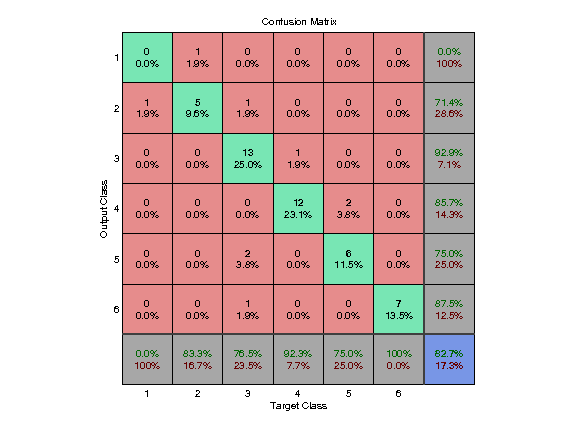
\includegraphics[scale=0.8]{../src/results/nominal/automobile_mc29.png}
				\caption{Matriz de confusión. Conjunto de datos Automobile. Clasificación nominal.}
				\label{fig:nomaut}
			\end{figure}
			
			\subsubsection{Conjunto de datos Balance Scale}
			
			En la Tabla \ref{tab:nombal} se muestran los resultados individuales de las 30 ejecuciones del algoritmo de clasificación nominal mediante una red neuronal artificial no ordinal para el conjunto de datos Balance Scale, donde se muestra el número de ejecuciones, el CCR, el MAE, el número de neuronas en capa oculta calculado y el tiempo total de la ejecución.\\
			
			\begin{table}[!htbp]
				\centering
				\CSVtotabular{../src/results/nominal/balance.csv}{l|r|r|r|r|r|r}{%
					\bfseries numIter &
					\bfseries CCR &
					\bfseries MAE &
					\bfseries NH &
					\bfseries CompTime\\\hline}{%
					\insertnumIter &
					\insertCCR &
					\insertMAE &
					\insertNH &
					\insertCompTime\\}{%
					\insertnumIter &
					\insertCCR &
					\insertMAE &
					\insertNH &
					\insertCompTime\\
					}
				\caption{Resultados individuales. Conjunto de datos Balance Scale. Clasificación nominal.}
				\label{tab:nombal}
			\end{table}
			
			La matriz de confusión para el mejor resultado del CCR obtenido de las 30 ejecuciones es la que se muestra en la Figura \ref{fig:nombal}.
			
			\begin{figure}[htbp]
				\centering
				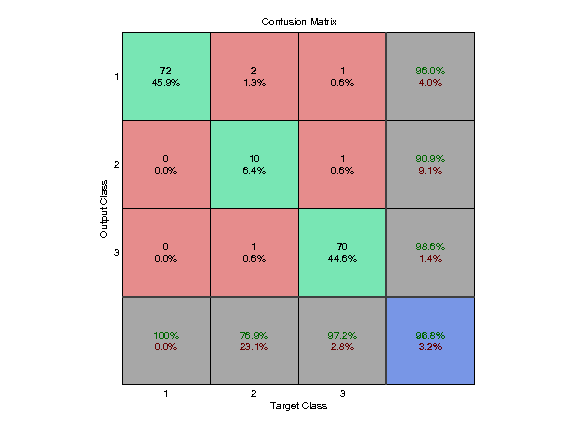
\includegraphics[scale=0.8]{../src/results/nominal/balance_mc6.png}
				\caption{Matriz de confusión. Conjunto de datos Balance Scale. Clasificación nominal.}
				\label{fig:nombal}
			\end{figure}
			
			\subsubsection{Conjunto de datos Bondrate}
			
			En la Tabla \ref{tab:nombon} se muestran los resultados individuales de las 30 ejecuciones del algoritmo de clasificación nominal mediante una red neuronal artificial no ordinal para el conjunto de datos Bondrate, donde se muestra el número de ejecuciones, el CCR, el MAE, el número de neuronas en capa oculta calculado y el tiempo total de la ejecución.\\
			
			\begin{table}[!htbp]
				\centering
				\CSVtotabular{../src/results/nominal/bondrate.csv}{l|r|r|r|r|r|r}{%
					\bfseries numIter &
					\bfseries CCR &
					\bfseries MAE &
					\bfseries NH &
					\bfseries CompTime\\\hline}{%
					\insertnumIter &
					\insertCCR &
					\insertMAE &
					\insertNH &
					\insertCompTime\\}{%
					\insertnumIter &
					\insertCCR &
					\insertMAE &
					\insertNH &
					\insertCompTime\\
					}
				\caption{Resultados individuales. Conjunto de datos Bondrate. Clasificación nominal.}
				\label{tab:nombon}
			\end{table}
			
			La matriz de confusión para el mejor resultado del CCR obtenido de las 30 ejecuciones es la que se muestra en la Figura \ref{fig:nombon}.
			
			\begin{figure}[htbp]
				\centering
				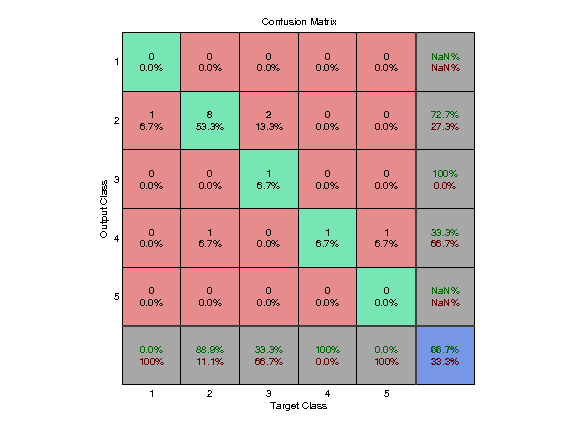
\includegraphics[scale=0.8]{../src/results/nominal/bondrate_mc1.png}
				\caption{Matriz de confusión. Conjunto de datos Bondrate. Clasificación nominal.}
				\label{fig:nombon}
			\end{figure}

			\subsubsection{Conjunto de datos Car}
			
			En la Tabla \ref{tab:nomcar} se muestran los resultados individuales de las 30 ejecuciones del algoritmo de clasificación nominal mediante una red neuronal artificial no ordinal para el conjunto de datos Car, donde se muestra el número de ejecuciones, el CCR, el MAE, el número de neuronas en capa oculta calculado y el tiempo total de la ejecución.\\
			
			\begin{table}[!htbp]
				\centering
				\CSVtotabular{../src/results/nominal/car.csv}{l|r|r|r|r|r|r}{%
					\bfseries numIter &
					\bfseries CCR &
					\bfseries MAE &
					\bfseries NH &
					\bfseries CompTime\\\hline}{%
					\insertnumIter &
					\insertCCR &
					\insertMAE &
					\insertNH &
					\insertCompTime\\}{%
					\insertnumIter &
					\insertCCR &
					\insertMAE &
					\insertNH &
					\insertCompTime\\
					}
				\caption{Resultados individuales. Conjunto de datos Car. Clasificación nominal.}
				\label{tab:nomcar}
			\end{table}
			
			La matriz de confusión para el mejor resultado del CCR obtenido de las 30 ejecuciones es la que se muestra en la Figura \ref{fig:nomcar}.
			
			\begin{figure}[htbp]
				\centering
				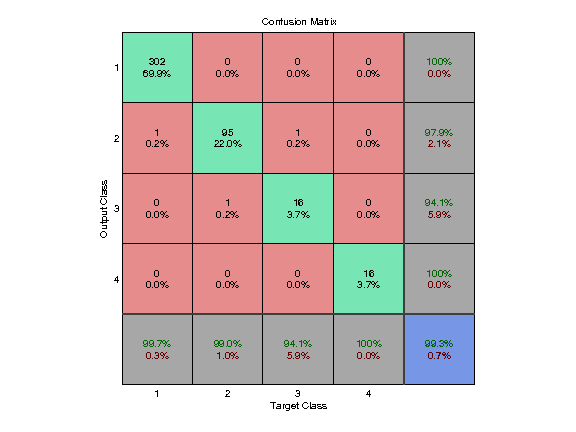
\includegraphics[scale=0.8]{../src/results/nominal/car_mc22.png}
				\caption{Matriz de confusión. Conjunto de datos Car. Clasificación nominal.}
				\label{fig:nomcar}
			\end{figure}

			\subsubsection{Conjunto de datos Contact lenses}
			
			En la Tabla \ref{tab:nomcon} se muestran los resultados individuales de las 30 ejecuciones del algoritmo de clasificación nominal mediante una red neuronal artificial no ordinal para el conjunto de datos Contact Lenses, donde se muestra el número de ejecuciones, el CCR, el MAE, el número de neuronas en capa oculta calculado y el tiempo total de la ejecución.\\
			
			\begin{table}[!htbp]
				\centering
				\CSVtotabular{../src/results/nominal/contact-lenses.csv}{l|r|r|r|r|r|r}{%
					\bfseries numIter &
					\bfseries CCR &
					\bfseries MAE &
					\bfseries NH &
					\bfseries CompTime\\\hline}{%
					\insertnumIter &
					\insertCCR &
					\insertMAE &
					\insertNH &
					\insertCompTime\\}{%
					\insertnumIter &
					\insertCCR &
					\insertMAE &
					\insertNH &
					\insertCompTime\\
					}
				\caption{Resultados individuales. Conjunto de datos Contact Lenses. Clasificación nominal.}
				\label{tab:nomcon}
			\end{table}
			
			La matriz de confusión para el mejor resultado del CCR obtenido de las 30 ejecuciones es la que se muestra en la Figura \ref{fig:nomcon}.
			
			\begin{figure}[htbp]
				\centering
				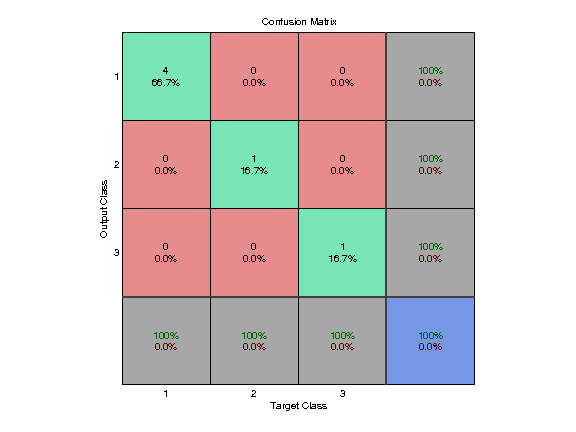
\includegraphics[scale=0.8]{../src/results/nominal/contact-lenses_mc2.png}
				\caption{Matriz de confusión. Conjunto de datos Contact Lenses. Clasificación nominal.}
				\label{fig:nomcon}
			\end{figure}

			\subsubsection{Conjunto de datos Depression}
			
			En la Tabla \ref{tab:nomdep} se muestran los resultados individuales de las 30 ejecuciones del algoritmo de clasificación nominal mediante una red neuronal artificial no ordinal para el conjunto de datos Depression, donde se muestra el número de ejecuciones, el CCR, el MAE, el número de neuronas en capa oculta calculado y el tiempo total de la ejecución.\\
			
			\begin{table}[!htbp]
				\centering
				\CSVtotabular{../src/results/nominal/depresion.csv}{l|r|r|r|r|r|r}{%
					\bfseries numIter &
					\bfseries CCR &
					\bfseries MAE &
					\bfseries NH &
					\bfseries CompTime\\\hline}{%
					\insertnumIter &
					\insertCCR &
					\insertMAE &
					\insertNH &
					\insertCompTime\\}{%
					\insertnumIter &
					\insertCCR &
					\insertMAE &
					\insertNH &
					\insertCompTime\\
					}
				\caption{Resultados individuales. Conjunto de datos Depression. Clasificación nominal.}
				\label{tab:nomdep}
			\end{table}
			
			La matriz de confusión para el mejor resultado del CCR obtenido de las 30 ejecuciones es la que se muestra en la Figura \ref{fig:nomdep}.
			
			\begin{figure}[htbp]
				\centering
				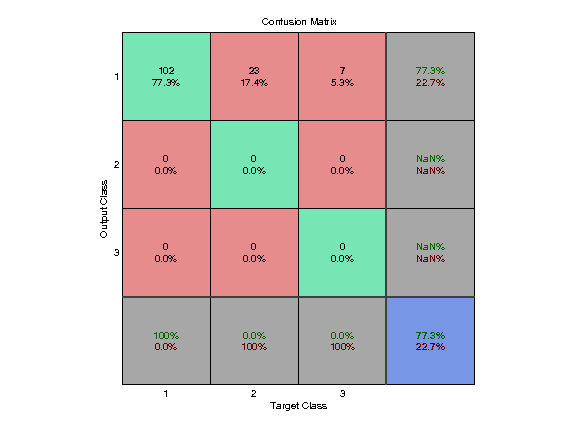
\includegraphics[scale=0.8]{../src/results/nominal/depresion_mc1.png}
				\caption{Matriz de confusión. Conjunto de datos Depression. Clasificación nominal.}
				\label{fig:nomdep}
			\end{figure}

			\subsubsection{Conjunto de datos ERA}
			
			En la Tabla \ref{tab:nomera} se muestran los resultados individuales de las 30 ejecuciones del algoritmo de clasificación nominal mediante una red neuronal artificial no ordinal para el conjunto de datos ERA, donde se muestra el número de ejecuciones, el CCR, el MAE, el número de neuronas en capa oculta calculado y el tiempo total de la ejecución.\\
			
			\begin{table}[!htbp]
				\centering
				\CSVtotabular{../src/results/nominal/ERA.csv}{l|r|r|r|r|r|r}{%
					\bfseries numIter &
					\bfseries CCR &
					\bfseries MAE &
					\bfseries NH &
					\bfseries CompTime\\\hline}{%
					\insertnumIter &
					\insertCCR &
					\insertMAE &
					\insertNH &
					\insertCompTime\\}{%
					\insertnumIter &
					\insertCCR &
					\insertMAE &
					\insertNH &
					\insertCompTime\\
					}
				\caption{Resultados individuales. Conjunto de datos ERA. Clasificación nominal.}
				\label{tab:nomera}
			\end{table}
			
			La matriz de confusión para el mejor resultado del CCR obtenido de las 30 ejecuciones es la que se muestra en la Figura \ref{fig:nomera}.
			
			\begin{figure}[htbp]
				\centering
				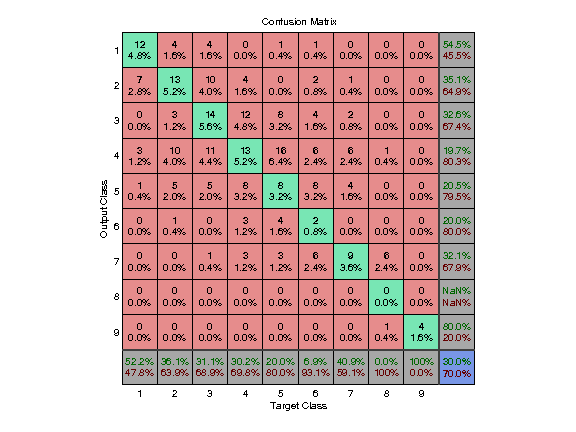
\includegraphics[scale=0.8]{../src/results/nominal/ERA_mc2.png}
				\caption{Matriz de confusión. Conjunto de datos ERA. Clasificación nominal.}
				\label{fig:nomera}
			\end{figure}

			\subsubsection{Conjunto de datos ESL}
			
			En la Tabla \ref{tab:nomesl} se muestran los resultados individuales de las 30 ejecuciones del algoritmo de clasificación nominal mediante una red neuronal artificial no ordinal para el conjunto de datos ESL, donde se muestra el número de ejecuciones, el CCR, el MAE, el número de neuronas en capa oculta calculado y el tiempo total de la ejecución.\\
			
			\begin{table}[!htbp]
				\centering
				\CSVtotabular{../src/results/nominal/ESL.csv}{l|r|r|r|r|r|r}{%
					\bfseries numIter &
					\bfseries CCR &
					\bfseries MAE &
					\bfseries NH &
					\bfseries CompTime\\\hline}{%
					\insertnumIter &
					\insertCCR &
					\insertMAE &
					\insertNH &
					\insertCompTime\\}{%
					\insertnumIter &
					\insertCCR &
					\insertMAE &
					\insertNH &
					\insertCompTime\\
					}
				\caption{Resultados individuales. Conjunto de datos ESL. Clasificación nominal.}
				\label{tab:nomesl}
			\end{table}
			
			La matriz de confusión para el mejor resultado del CCR obtenido de las 30 ejecuciones es la que se muestra en la Figura \ref{fig:nomesl}.
			
			\begin{figure}[htbp]
				\centering
				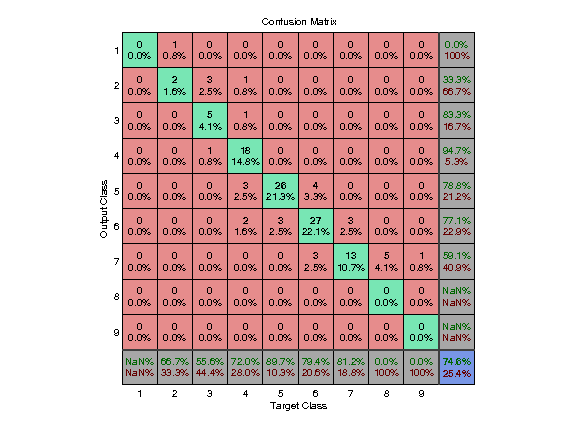
\includegraphics[scale=0.8]{../src/results/nominal/ESL_mc12.png}
				\caption{Matriz de confusión. Conjunto de datos ESL. Clasificación nominal.}
				\label{fig:nomesl}
			\end{figure}

			\subsubsection{Conjunto de datos Eucalyptus}
			
			En la Tabla \ref{tab:nomeuc} se muestran los resultados individuales de las 30 ejecuciones del algoritmo de clasificación nominal mediante una red neuronal artificial no ordinal para el conjunto de datos Eucalyptus, donde se muestra el número de ejecuciones, el CCR, el MAE, el número de neuronas en capa oculta calculado y el tiempo total de la ejecución.\\
			
			\begin{table}[!htbp]
				\centering
				\CSVtotabular{../src/results/nominal/eucalyptus.csv}{l|r|r|r|r|r|r}{%
					\bfseries numIter &
					\bfseries CCR &
					\bfseries MAE &
					\bfseries NH &
					\bfseries CompTime\\\hline}{%
					\insertnumIter &
					\insertCCR &
					\insertMAE &
					\insertNH &
					\insertCompTime\\}{%
					\insertnumIter &
					\insertCCR &
					\insertMAE &
					\insertNH &
					\insertCompTime\\
					}
				\caption{Resultados individuales. Conjunto de datos Eucalyptus. Clasificación nominal.}
				\label{tab:nomeuc}
			\end{table}
			
			La matriz de confusión para el mejor resultado del CCR obtenido de las 30 ejecuciones es la que se muestra en la Figura \ref{fig:nomeuc}.
			
			\begin{figure}[htbp]
				\centering
				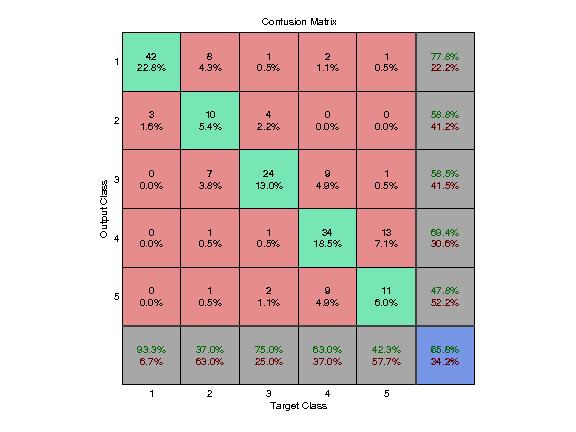
\includegraphics[scale=0.8]{../src/results/nominal/eucalyptus_mc1.png}
				\caption{Matriz de confusión. Conjunto de datos Eucalyptus. Clasificación nominal.}
				\label{fig:nomeuc}
			\end{figure}

			\subsubsection{Conjunto de datos LEV}
			
			En la Tabla \ref{tab:nomlev} se muestran los resultados individuales de las 30 ejecuciones del algoritmo de clasificación nominal mediante una red neuronal artificial no ordinal para el conjunto de datos LEV, donde se muestra el número de ejecuciones, el CCR, el MAE, el número de neuronas en capa oculta calculado y el tiempo total de la ejecución.\\
			
			\begin{table}[!htbp]
				\centering
				\CSVtotabular{../src/results/nominal/LEV.csv}{l|r|r|r|r|r|r}{%
					\bfseries numIter &
					\bfseries CCR &
					\bfseries MAE &
					\bfseries NH &
					\bfseries CompTime\\\hline}{%
					\insertnumIter &
					\insertCCR &
					\insertMAE &
					\insertNH &
					\insertCompTime\\}{%
					\insertnumIter &
					\insertCCR &
					\insertMAE &
					\insertNH &
					\insertCompTime\\
					}
				\caption{Resultados individuales. Conjunto de datos LEV. Clasificación nominal.}
				\label{tab:nomlev}
			\end{table}
			
			La matriz de confusión para el mejor resultado del CCR obtenido de las 30 ejecuciones es la que se muestra en la Figura \ref{fig:nomlev}.
			
			\begin{figure}[htbp]
				\centering
				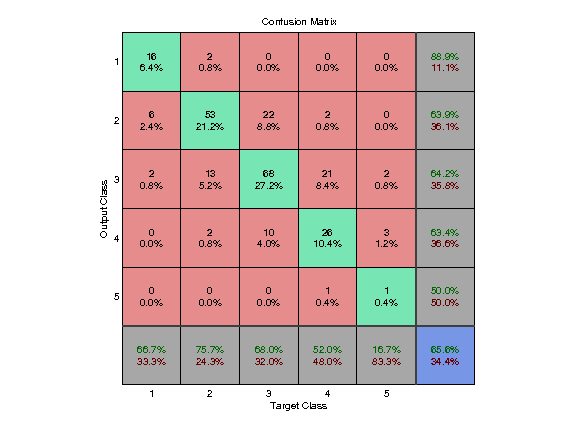
\includegraphics[scale=0.8]{../src/results/nominal/LEV_mc28.png}
				\caption{Matriz de confusión. Conjunto de datos LEV. Clasificación nominal.}
				\label{fig:nomlev}
			\end{figure}

			\subsubsection{Conjunto de datos New Thyroid}
			
			En la Tabla \ref{tab:nomnew} se muestran los resultados individuales de las 30 ejecuciones del algoritmo de clasificación nominal mediante una red neuronal artificial no ordinal para el conjunto de datos New Thyroid, donde se muestra el número de ejecuciones, el CCR, el MAE, el número de neuronas en capa oculta calculado y el tiempo total de la ejecución.\\
			
			\begin{table}[!htbp]
				\centering
				\CSVtotabular{../src/results/nominal/newthyroid.csv}{l|r|r|r|r|r|r}{%
					\bfseries numIter &
					\bfseries CCR &
					\bfseries MAE &
					\bfseries NH &
					\bfseries CompTime\\\hline}{%
					\insertnumIter &
					\insertCCR &
					\insertMAE &
					\insertNH &
					\insertCompTime\\}{%
					\insertnumIter &
					\insertCCR &
					\insertMAE &
					\insertNH &
					\insertCompTime\\
					}
				\caption{Resultados individuales. Conjunto de datos New Thyroid. Clasificación nominal.}
				\label{tab:nomnew}
			\end{table}
			
			La matriz de confusión para el mejor resultado del CCR obtenido de las 30 ejecuciones es la que se muestra en la Figura \ref{fig:nomnew}.
			
			\begin{figure}[htbp]
				\centering
				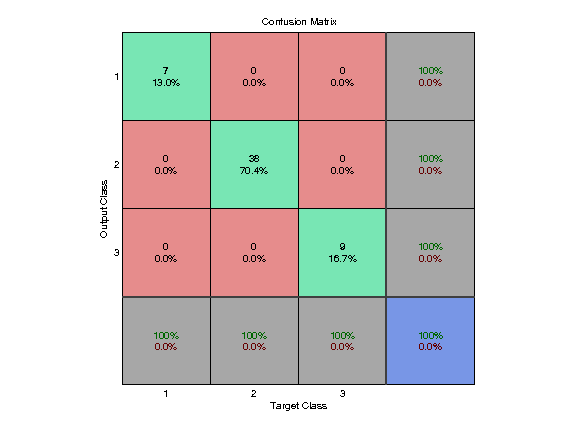
\includegraphics[scale=0.8]{../src/results/nominal/newthyroid_mc14.png}
				\caption{Matriz de confusión. Conjunto de datos New Thyroid. Clasificación nominal.}
				\label{fig:nomnew}
			\end{figure}

			\subsubsection{Conjunto de datos Pasture}
			
			En la Tabla \ref{tab:nompas} se muestran los resultados individuales de las 30 ejecuciones del algoritmo de clasificación nominal mediante una red neuronal artificial no ordinal para el conjunto de datos Pasture, donde se muestra el número de ejecuciones, el CCR, el MAE, el número de neuronas en capa oculta calculado y el tiempo total de la ejecución.\\
			
			\begin{table}[!htbp]
				\centering
				\CSVtotabular{../src/results/nominal/pasture.csv}{l|r|r|r|r|r|r}{%
					\bfseries numIter &
					\bfseries CCR &
					\bfseries MAE &
					\bfseries NH &
					\bfseries CompTime\\\hline}{%
					\insertnumIter &
					\insertCCR &
					\insertMAE &
					\insertNH &
					\insertCompTime\\}{%
					\insertnumIter &
					\insertCCR &
					\insertMAE &
					\insertNH &
					\insertCompTime\\
					}
				\caption{Resultados individuales. Conjunto de datos Pasture. Clasificación nominal.}
				\label{tab:nompas}
			\end{table}
			
			La matriz de confusión para el mejor resultado del CCR obtenido de las 30 ejecuciones es la que se muestra en la Figura \ref{fig:nompas}.
			
			\begin{figure}[htbp]
				\centering
				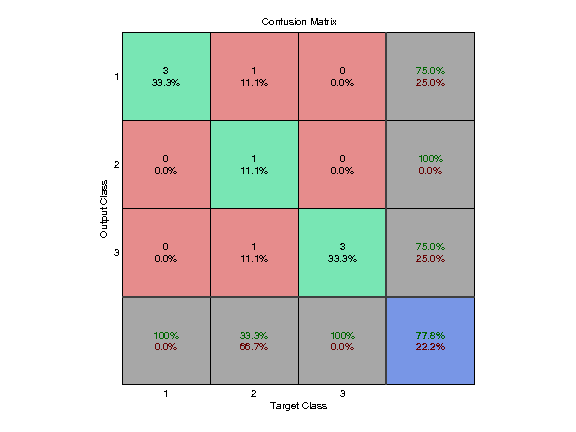
\includegraphics[scale=0.8]{../src/results/nominal/pasture_mc7.png}
				\caption{Matriz de confusión. Conjunto de datos Pasture. Clasificación nominal.}
				\label{fig:nompas}
			\end{figure}

			\subsubsection{Conjunto de datos Squash Stored}
			
			En la Tabla \ref{tab:nomsqu} se muestran los resultados individuales de las 30 ejecuciones del algoritmo de clasificación nominal mediante una red neuronal artificial no ordinal para el conjunto de datos Squash Stored, donde se muestra el número de ejecuciones, el CCR, el MAE, el número de neuronas en capa oculta calculado y el tiempo total de la ejecución.\\
			
			\begin{table}[!htbp]
				\centering
				\CSVtotabular{../src/results/nominal/squash-stored.csv}{l|r|r|r|r|r|r}{%
					\bfseries numIter &
					\bfseries CCR &
					\bfseries MAE &
					\bfseries NH &
					\bfseries CompTime\\\hline}{%
					\insertnumIter &
					\insertCCR &
					\insertMAE &
					\insertNH &
					\insertCompTime\\}{%
					\insertnumIter &
					\insertCCR &
					\insertMAE &
					\insertNH &
					\insertCompTime\\
					}
				\caption{Resultados individuales. Conjunto de datos Squash Stored. Clasificación nominal.}
				\label{tab:nomsqu}
			\end{table}
			
			La matriz de confusión para el mejor resultado del CCR obtenido de las 30 ejecuciones es la que se muestra en la Figura \ref{fig:nomsqu}.
			
			\begin{figure}[htbp]
				\centering
				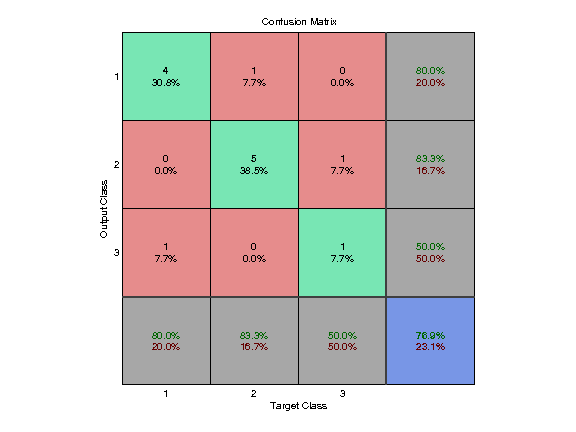
\includegraphics[scale=0.8]{../src/results/nominal/squash-stored_mc25.png}
				\caption{Matriz de confusión. Conjunto de datos Squash Stored. Clasificación nominal.}
				\label{fig:nomsqu}
			\end{figure}

			\subsubsection{Conjunto de datos Squash Unstored}
			
			En la Tabla \ref{tab:nomsqua} se muestran los resultados individuales de las 30 ejecuciones del algoritmo de clasificación nominal mediante una red neuronal artificial no ordinal para el conjunto de datos Squash Unstored, donde se muestra el número de ejecuciones, el CCR, el MAE, el número de neuronas en capa oculta calculado y el tiempo total de la ejecución.\\
			
			\begin{table}[!htbp]
				\centering
				\CSVtotabular{../src/results/nominal/squash-unstored.csv}{l|r|r|r|r|r|r}{%
					\bfseries numIter &
					\bfseries CCR &
					\bfseries MAE &
					\bfseries NH &
					\bfseries CompTime\\\hline}{%
					\insertnumIter &
					\insertCCR &
					\insertMAE &
					\insertNH &
					\insertCompTime\\}{%
					\insertnumIter &
					\insertCCR &
					\insertMAE &
					\insertNH &
					\insertCompTime\\
					}
				\caption{Resultados individuales. Conjunto de datos Squash Unstored. Clasificación nominal.}
				\label{tab:nomsqua}
			\end{table}
			
			La matriz de confusión para el mejor resultado del CCR obtenido de las 30 ejecuciones es la que se muestra en la Figura \ref{fig:nomsqua}.
			
			\begin{figure}[htbp]
				\centering
				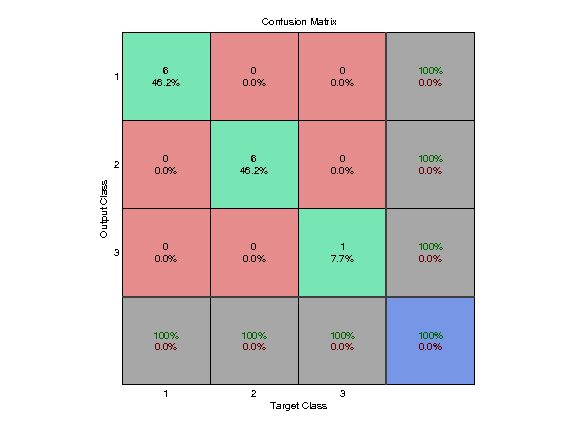
\includegraphics[scale=0.8]{../src/results/nominal/squash-unstored_mc20.png}
				\caption{Matriz de confusión. Conjunto de datos Squash Unstored. Clasificación nominal.}
				\label{fig:nomsqua}
			\end{figure}

			\subsubsection{Conjunto de datos SWD}
			
			En la Tabla \ref{tab:nomswd} se muestran los resultados individuales de las 30 ejecuciones del algoritmo de clasificación nominal mediante una red neuronal artificial no ordinal para el conjunto de datos SWD, donde se muestra el número de ejecuciones, el CCR, el MAE, el número de neuronas en capa oculta calculado y el tiempo total de la ejecución.\\
			
			\begin{table}[!htbp]
				\centering
				\CSVtotabular{../src/results/nominal/SWD.csv}{l|r|r|r|r|r|r}{%
					\bfseries numIter &
					\bfseries CCR &
					\bfseries MAE &
					\bfseries NH &
					\bfseries CompTime\\\hline}{%
					\insertnumIter &
					\insertCCR &
					\insertMAE &
					\insertNH &
					\insertCompTime\\}{%
					\insertnumIter &
					\insertCCR &
					\insertMAE &
					\insertNH &
					\insertCompTime\\
					}
				\caption{Resultados individuales. Conjunto de datos SWD. Clasificación nominal.}
				\label{tab:nomswd}
			\end{table}
			
			La matriz de confusión para el mejor resultado del CCR obtenido de las 30 ejecuciones es la que se muestra en la Figura \ref{fig:nomswd}.
			
			\begin{figure}[htbp]
				\centering
				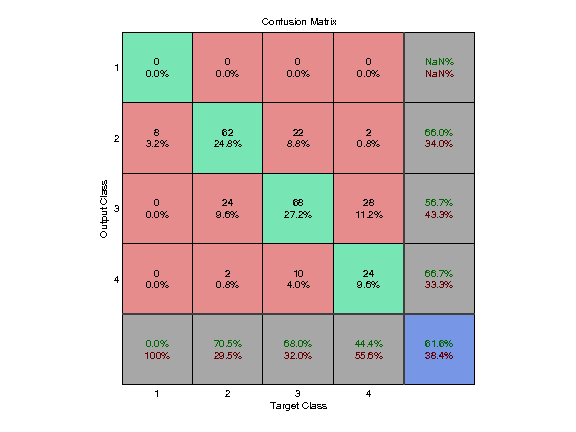
\includegraphics[scale=0.8]{../src/results/nominal/SWD_mc7.png}
				\caption{Matriz de confusión. Conjunto de datos SWD. Clasificación nominal.}
				\label{fig:nomswd}
			\end{figure}

			\subsubsection{Conjunto de datos TAE}
			
			En la Tabla \ref{tab:nomtae} se muestran los resultados individuales de las 30 ejecuciones del algoritmo de clasificación nominal mediante una red neuronal artificial no ordinal para el conjunto de datos TAE, donde se muestra el número de ejecuciones, el CCR, el MAE, el número de neuronas en capa oculta calculado y el tiempo total de la ejecución.\\
			
			\begin{table}[!htbp]
				\centering
				\CSVtotabular{../src/results/nominal/tae.csv}{l|r|r|r|r|r|r}{%
					\bfseries numIter &
					\bfseries CCR &
					\bfseries MAE &
					\bfseries NH &
					\bfseries CompTime\\\hline}{%
					\insertnumIter &
					\insertCCR &
					\insertMAE &
					\insertNH &
					\insertCompTime\\}{%
					\insertnumIter &
					\insertCCR &
					\insertMAE &
					\insertNH &
					\insertCompTime\\
					}
				\caption{Resultados individuales. Conjunto de datos TAE. Clasificación nominal.}
				\label{tab:nomtae}
			\end{table}
			
			La matriz de confusión para el mejor resultado del CCR obtenido de las 30 ejecuciones es la que se muestra en la Figura \ref{fig:nomtae}.
			
			\begin{figure}[htbp]
				\centering
				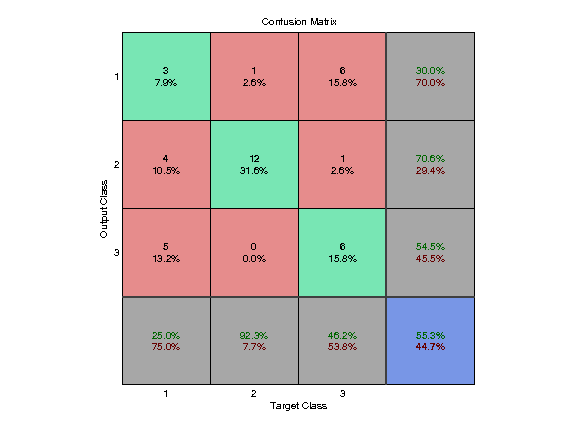
\includegraphics[scale=0.8]{../src/results/nominal/tae_mc16.png}
				\caption{Matriz de confusión. Conjunto de datos TAE. Clasificación nominal.}
				\label{fig:nomtae}
			\end{figure}

			\subsubsection{Conjunto de datos Thyroid}
			
			En la Tabla \ref{tab:nomthy} se muestran los resultados individuales de las 30 ejecuciones del algoritmo de clasificación nominal mediante una red neuronal artificial no ordinal para el conjunto de datos Thyroid, donde se muestra el número de ejecuciones, el CCR, el MAE, el número de neuronas en capa oculta calculado y el tiempo total de la ejecución.\\
			
			\begin{table}[!htbp]
				\centering
				\CSVtotabular{../src/results/nominal/thyroid.csv}{l|r|r|r|r|r|r}{%
					\bfseries numIter &
					\bfseries CCR &
					\bfseries MAE &
					\bfseries NH &
					\bfseries CompTime\\\hline}{%
					\insertnumIter &
					\insertCCR &
					\insertMAE &
					\insertNH &
					\insertCompTime\\}{%
					\insertnumIter &
					\insertCCR &
					\insertMAE &
					\insertNH &
					\insertCompTime\\
					}
				\caption{Resultados individuales. Conjunto de datos Thyroid. Clasificación nominal.}
				\label{tab:nomthy}
			\end{table}
			
			La matriz de confusión para el mejor resultado del CCR obtenido de las 30 ejecuciones es la que se muestra en la Figura \ref{fig:nomthy}.
			
			\begin{figure}[htbp]
				\centering
				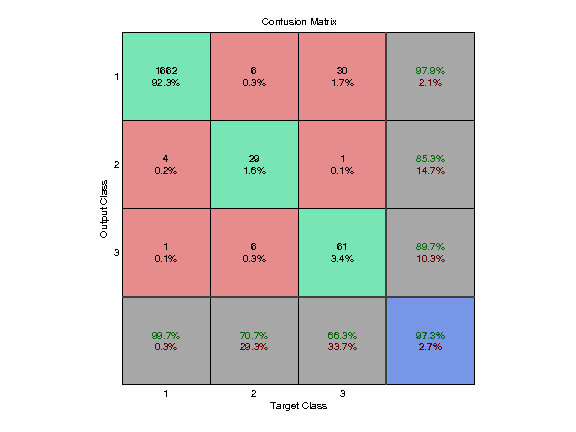
\includegraphics[scale=0.8]{../src/results/nominal/thyroid_mc29.png}
				\caption{Matriz de confusión. Conjunto de datos Thyroid. Clasificación nominal.}
				\label{fig:nomthy}
			\end{figure}

			\subsubsection{Conjunto de datos Wine Quality Red}
			
			En la Tabla \ref{tab:nomred} se muestran los resultados individuales de las 30 ejecuciones del algoritmo de clasificación nominal mediante una red neuronal artificial no ordinal para el conjunto de datos Wine Quality Red, donde se muestra el número de ejecuciones, el CCR, el MAE, el número de neuronas en capa oculta calculado y el tiempo total de la ejecución.\\
			
			\begin{table}[!htbp]
				\centering
				\CSVtotabular{../src/results/nominal/winequality-red.csv}{l|r|r|r|r|r|r}{%
					\bfseries numIter &
					\bfseries CCR &
					\bfseries MAE &
					\bfseries NH &
					\bfseries CompTime\\\hline}{%
					\insertnumIter &
					\insertCCR &
					\insertMAE &
					\insertNH &
					\insertCompTime\\}{%
					\insertnumIter &
					\insertCCR &
					\insertMAE &
					\insertNH &
					\insertCompTime\\
					}
				\caption{Resultados individuales. Conjunto de datos Wine Quality Red. Clasificación nominal.}
				\label{tab:nomred}
			\end{table}
			
			La matriz de confusión para el mejor resultado del CCR obtenido de las 30 ejecuciones es la que se muestra en la Figura \ref{fig:nomred}.
			
			\begin{figure}[htbp]
				\centering
				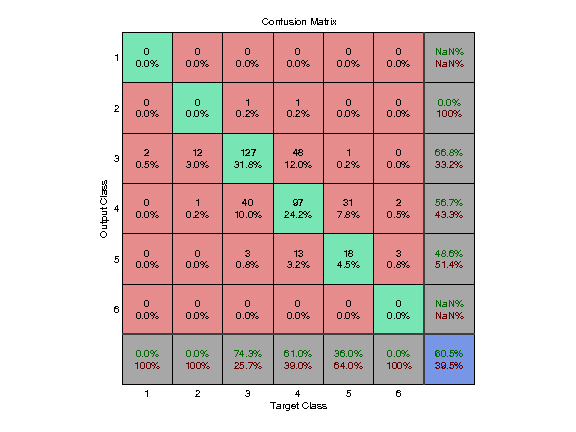
\includegraphics[scale=0.8]{../src/results/nominal/winequality-red_mc1.png}
				\caption{Matriz de confusión. Conjunto de datos Wine Quality Red. Clasificación nominal.}
				\label{fig:nomred}
			\end{figure}

			\subsubsection{Conjunto de datos Wine Quality White}
			
			En la Tabla \ref{tab:nomwhi} se muestran los resultados individuales de las 30 ejecuciones del algoritmo de clasificación nominal mediante una red neuronal artificial no ordinal para el conjunto de datos Wine Quality White, donde se muestra el número de ejecuciones, el CCR, el MAE, el número de neuronas en capa oculta calculado y el tiempo total de la ejecución.\\
			
			\begin{table}[!htbp]
				\centering
				\CSVtotabular{../src/results/nominal/winequality-white.csv}{l|r|r|r|r|r|r}{%
					\bfseries numIter &
					\bfseries CCR &
					\bfseries MAE &
					\bfseries NH &
					\bfseries CompTime\\\hline}{%
					\insertnumIter &
					\insertCCR &
					\insertMAE &
					\insertNH &
					\insertCompTime\\}{%
					\insertnumIter &
					\insertCCR &
					\insertMAE &
					\insertNH &
					\insertCompTime\\
					}
				\caption{Resultados individuales. Conjunto de datos Wine Quality White. Clasificación nominal.}
				\label{tab:nomwhi}
			\end{table}
			
			La matriz de confusión para el mejor resultado del CCR obtenido de las 30 ejecuciones es la que se muestra en la Figura \ref{fig:nomwhi}.
			
			\begin{figure}[htbp]
				\centering
				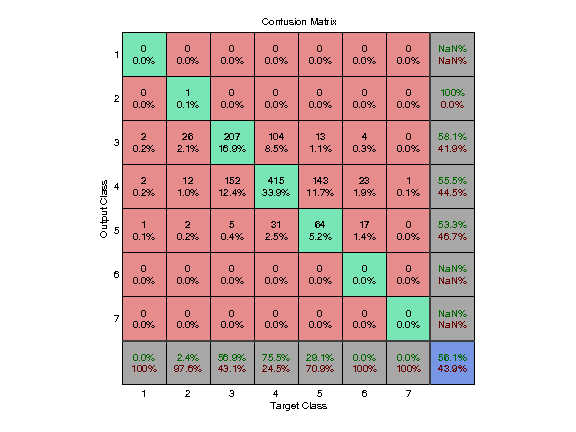
\includegraphics[scale=0.8]{../src/results/nominal/winequality-white_mc14.png}
				\caption{Matriz de confusión. Conjunto de datos Wine Quality White. Clasificación nominal.}
				\label{fig:nomwhi}
			\end{figure}
		
		\subsection{Clasificación Ordinal}
		
			Para cada uno de los conjuntos se mostrarán los datos obtenidos correspondientes a aplicar un modelo de clasificación donde se tiene en cuenta el orden de las etiquetas y la matriz de confusión del mejor resultado.
	
			\subsubsection{Conjunto de datos Automobile}
			
			En la Tabla \ref{tab:ordaut} se muestran los resultados individuales de las 30 ejecuciones del algoritmo de regresión ordinal ORNNet mediante una red neuronal artificial ordinal para el conjunto de datos Automobile, donde se muestra el número de ejecuciones, el CCR, el MAE, el número de neuronas en capa oculta calculado y el tiempo total de la ejecución.\\
			
			\begin{table}[!htbp]
				\centering
				\CSVtotabular{../src/results/ordinal/automobile.csv}{l|r|r|r|r|r|r}{%
					\bfseries numIter &
					\bfseries CCR &
					\bfseries MAE &
					\bfseries NH &
					\bfseries CompTime\\\hline}{%
					\insertnumIter &
					\insertCCR &
					\insertMAE &
					\insertNH &
					\insertCompTime\\}{%
					\insertnumIter &
					\insertCCR &
					\insertMAE &
					\insertNH &
					\insertCompTime\\
					}
				\caption{Resultados individuales. Conjunto de datos Automobile. Clasificación ordinal.}
				\label{tab:ordaut}
			\end{table}
			
			La matriz de confusión para el mejor resultado del CCR obtenido de las 30 ejecuciones es la que se muestra en la Figura \ref{fig:ordaut}.
			
			\begin{figure}[htbp]
				\centering
				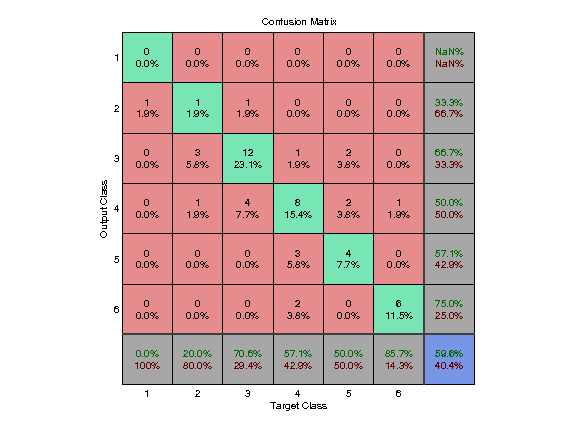
\includegraphics[scale=0.8]{../src/results/ordinal/automobile_mc1.png}
				\caption{Matriz de confusión. Conjunto de datos Automobile. Clasificación ordinal.}
				\label{fig:ordaut}
			\end{figure}
			
			\subsubsection{Conjunto de datos Balance Scale}
			
			En la Tabla \ref{tab:ordbal} se muestran los resultados individuales de las 30 ejecuciones del algoritmo de regresión ordinal ORNNet mediante una red neuronal artificial ordinal para el conjunto de datos Balance Scale, donde se muestra el número de ejecuciones, el CCR, el MAE, el número de neuronas en capa oculta calculado y el tiempo total de la ejecución.\\
			
			\begin{table}[!htbp]
				\centering
				\CSVtotabular{../src/results/ordinal/balance.csv}{l|r|r|r|r|r|r}{%
					\bfseries numIter &
					\bfseries CCR &
					\bfseries MAE &
					\bfseries NH &
					\bfseries CompTime\\\hline}{%
					\insertnumIter &
					\insertCCR &
					\insertMAE &
					\insertNH &
					\insertCompTime\\}{%
					\insertnumIter &
					\insertCCR &
					\insertMAE &
					\insertNH &
					\insertCompTime\\
					}
				\caption{Resultados individuales. Conjunto de datos Balance Scale. Clasificación ordinal.}
				\label{tab:ordbal}
			\end{table}
			
			La matriz de confusión para el mejor resultado del CCR obtenido de las 30 ejecuciones es la que se muestra en la Figura \ref{fig:ordbal}.
			
			\begin{figure}[htbp]
				\centering
				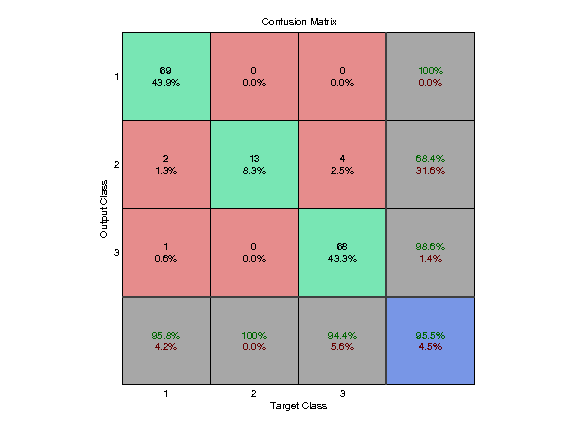
\includegraphics[scale=0.8]{../src/results/ordinal/balance_mc1.png}
				\caption{Matriz de confusión. Conjunto de datos Balance Scale. Clasificación ordinal.}
				\label{fig:ordbal}
			\end{figure}
			
			\subsubsection{Conjunto de datos Bondrate}
			
			En la Tabla \ref{tab:ordbon} se muestran los resultados individuales de las 30 ejecuciones del algoritmo de regresión ordinal ORNNet mediante una red neuronal artificial ordinal para el conjunto de datos Bondrate, donde se muestra el número de ejecuciones, el CCR, el MAE, el número de neuronas en capa oculta calculado y el tiempo total de la ejecución.\\
			
			\begin{table}[!htbp]
				\centering
				\CSVtotabular{../src/results/ordinal/bondrate.csv}{l|r|r|r|r|r|r}{%
					\bfseries numIter &
					\bfseries CCR &
					\bfseries MAE &
					\bfseries NH &
					\bfseries CompTime\\\hline}{%
					\insertnumIter &
					\insertCCR &
					\insertMAE &
					\insertNH &
					\insertCompTime\\}{%
					\insertnumIter &
					\insertCCR &
					\insertMAE &
					\insertNH &
					\insertCompTime\\
					}
				\caption{Resultados individuales. Conjunto de datos Bondrate. Clasificación ordinal.}
				\label{tab:ordbon}
			\end{table}
			
			La matriz de confusión para el mejor resultado del CCR obtenido de las 30 ejecuciones es la que se muestra en la Figura \ref{fig:ordbon}.
			
			\begin{figure}[htbp]
				\centering
				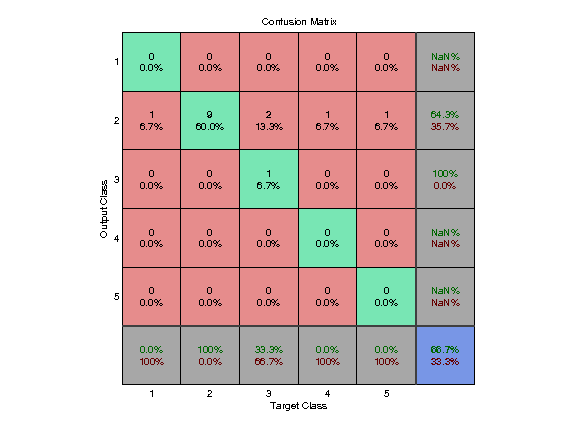
\includegraphics[scale=0.8]{../src/results/ordinal/bondrate_mc1.png}
				\caption{Matriz de confusión. Conjunto de datos Bondrate. Clasificación ordinal.}
				\label{fig:ordbon}
			\end{figure}
			
			\subsubsection{Conjunto de datos Car}
			
			En la Tabla \ref{tab:ordcar} se muestran los resultados individuales de las 30 ejecuciones del algoritmo de regresión ordinal ORNNet mediante una red neuronal artificial ordinal para el conjunto de datos Car, donde se muestra el número de ejecuciones, el CCR, el MAE, el número de neuronas en capa oculta calculado y el tiempo total de la ejecución.\\
			
			\begin{table}[!htbp]
				\centering
				\CSVtotabular{../src/results/ordinal/car.csv}{l|r|r|r|r|r|r}{%
					\bfseries numIter &
					\bfseries CCR &
					\bfseries MAE &
					\bfseries NH &
					\bfseries CompTime\\\hline}{%
					\insertnumIter &
					\insertCCR &
					\insertMAE &
					\insertNH &
					\insertCompTime\\}{%
					\insertnumIter &
					\insertCCR &
					\insertMAE &
					\insertNH &
					\insertCompTime\\
					}
				\caption{Resultados individuales. Conjunto de datos Car. Clasificación ordinal.}
				\label{tab:ordcar}
			\end{table}
			
			La matriz de confusión para el mejor resultado del CCR obtenido de las 30 ejecuciones es la que se muestra en la Figura \ref{fig:ordcar}.
			
			\begin{figure}[htbp]
				\centering
				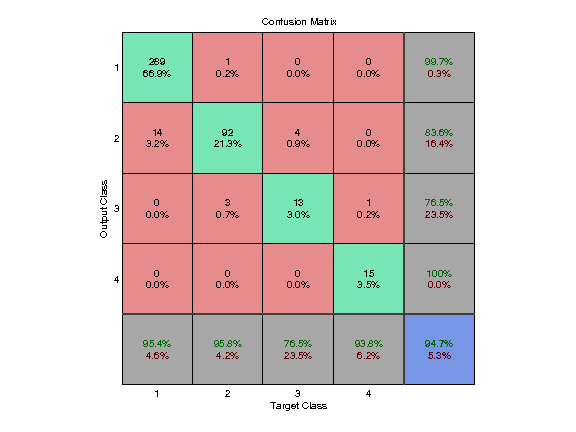
\includegraphics[scale=0.8]{../src/results/ordinal/car_mc1.png}
				\caption{Matriz de confusión. Conjunto de datos CAR. Clasificación ordinal.}
				\label{fig:ordcar}
			\end{figure}
			
			\subsubsection{Conjunto de datos Contact lenses}
			
			En la Tabla \ref{tab:ordcon} se muestran los resultados individuales de las 30 ejecuciones del algoritmo de regresión ordinal ORNNet mediante una red neuronal artificial ordinal para el conjunto de datos Contact Lenses, donde se muestra el número de ejecuciones, el CCR, el MAE, el número de neuronas en capa oculta calculado y el tiempo total de la ejecución.\\
			
			\begin{table}[!htbp]
				\centering
				\CSVtotabular{../src/results/ordinal/contact-lenses.csv}{l|r|r|r|r|r|r}{%
					\bfseries numIter &
					\bfseries CCR &
					\bfseries MAE &
					\bfseries NH &
					\bfseries CompTime\\\hline}{%
					\insertnumIter &
					\insertCCR &
					\insertMAE &
					\insertNH &
					\insertCompTime\\}{%
					\insertnumIter &
					\insertCCR &
					\insertMAE &
					\insertNH &
					\insertCompTime\\
					}
				\caption{Resultados individuales. Conjunto de datos Contact Lenses. Clasificación ordinal.}
				\label{tab:ordcon}
			\end{table}
			
			La matriz de confusión para el mejor resultado del CCR obtenido de las 30 ejecuciones es la que se muestra en la Figura \ref{fig:ordcon}.
			
			\begin{figure}[htbp]
				\centering
				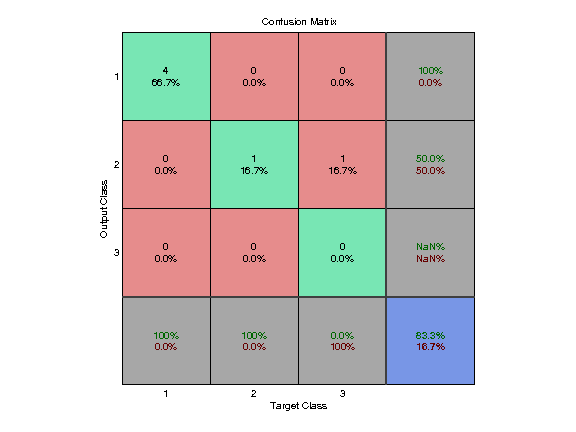
\includegraphics[scale=0.8]{../src/results/ordinal/contact-lenses_mc1.png}
				\caption{Matriz de confusión. Conjunto de datos Contact Lenses. Clasificación ordinal.}
				\label{fig:ordcon}
			\end{figure}
			
			\subsubsection{Conjunto de datos Depression}
			
			En la Tabla \ref{tab:orddep} se muestran los resultados individuales de las 30 ejecuciones del algoritmo de regresión ordinal ORNNet mediante una red neuronal artificial ordinal para el conjunto de datos Depression, donde se muestra el número de ejecuciones, el CCR, el MAE, el número de neuronas en capa oculta calculado y el tiempo total de la ejecución.\\
			
			\begin{table}[!htbp]
				\centering
				\CSVtotabular{../src/results/ordinal/depresion.csv}{l|r|r|r|r|r|r}{%
					\bfseries numIter &
					\bfseries CCR &
					\bfseries MAE &
					\bfseries NH &
					\bfseries CompTime\\\hline}{%
					\insertnumIter &
					\insertCCR &
					\insertMAE &
					\insertNH &
					\insertCompTime\\}{%
					\insertnumIter &
					\insertCCR &
					\insertMAE &
					\insertNH &
					\insertCompTime\\
					}
				\caption{Resultados individuales. Conjunto de datos Depression. Clasificación ordinal.}
				\label{tab:orddep}
			\end{table}
			
			La matriz de confusión para el mejor resultado del CCR obtenido de las 30 ejecuciones es la que se muestra en la Figura \ref{fig:orddep}.
			
			\begin{figure}[htbp]
				\centering
				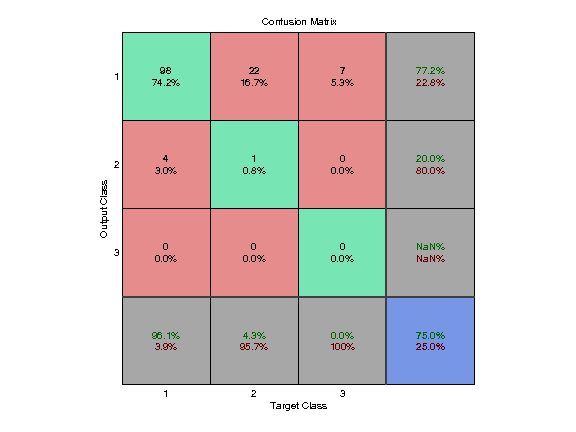
\includegraphics[scale=0.8]{../src/results/ordinal/depresion_mc1.png}
				\caption{Matriz de confusión. Conjunto de datos Depression. Clasificación ordinal.}
				\label{fig:orddep}
			\end{figure}
			
			\subsubsection{Conjunto de datos ERA}
			
			En la Tabla \ref{tab:ordera} se muestran los resultados individuales de las 30 ejecuciones del algoritmo de regresión ordinal ORNNet mediante una red neuronal artificial ordinal para el conjunto de datos ERA, donde se muestra el número de ejecuciones, el CCR, el MAE, el número de neuronas en capa oculta calculado y el tiempo total de la ejecución.\\
			
			\begin{table}[!htbp]
				\centering
				\CSVtotabular{../src/results/ordinal/ERA.csv}{l|r|r|r|r|r|r}{%
					\bfseries numIter &
					\bfseries CCR &
					\bfseries MAE &
					\bfseries NH &
					\bfseries CompTime\\\hline}{%
					\insertnumIter &
					\insertCCR &
					\insertMAE &
					\insertNH &
					\insertCompTime\\}{%
					\insertnumIter &
					\insertCCR &
					\insertMAE &
					\insertNH &
					\insertCompTime\\
					}
				\caption{Resultados individuales. Conjunto de datos ERA. Clasificación ordinal.}
				\label{tab:ordera}
			\end{table}
			
			La matriz de confusión para el mejor resultado del CCR obtenido de las 30 ejecuciones es la que se muestra en la Figura \ref{fig:ordera}.
			
			\begin{figure}[htbp]
				\centering
				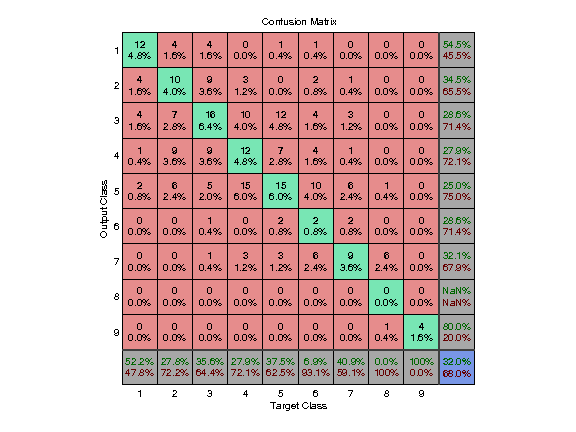
\includegraphics[scale=0.8]{../src/results/ordinal/ERA_mc1.png}
				\caption{Matriz de confusión. Conjunto de datos ERA. Clasificación ordinal.}
				\label{fig:ordera}
			\end{figure}
			
			\subsubsection{Conjunto de datos ESL}
			
			En la Tabla \ref{tab:ordesl} se muestran los resultados individuales de las 30 ejecuciones del algoritmo de regresión ordinal ORNNet mediante una red neuronal artificial ordinal para el conjunto de datos ESL, donde se muestra el número de ejecuciones, el CCR, el MAE, el número de neuronas en capa oculta calculado y el tiempo total de la ejecución.\\
			
			\begin{table}[!htbp]
				\centering
				\CSVtotabular{../src/results/ordinal/ESL.csv}{l|r|r|r|r|r|r}{%
					\bfseries numIter &
					\bfseries CCR &
					\bfseries MAE &
					\bfseries NH &
					\bfseries CompTime\\\hline}{%
					\insertnumIter &
					\insertCCR &
					\insertMAE &
					\insertNH &
					\insertCompTime\\}{%
					\insertnumIter &
					\insertCCR &
					\insertMAE &
					\insertNH &
					\insertCompTime\\
					}
				\caption{Resultados individuales. Conjunto de datos ESL. Clasificación ordinal.}
				\label{tab:ordesl}
			\end{table}
			
			La matriz de confusión para el mejor resultado del CCR obtenido de las 30 ejecuciones es la que se muestra en la Figura \ref{fig:ordesl}.
			
			\begin{figure}[htbp]
				\centering
				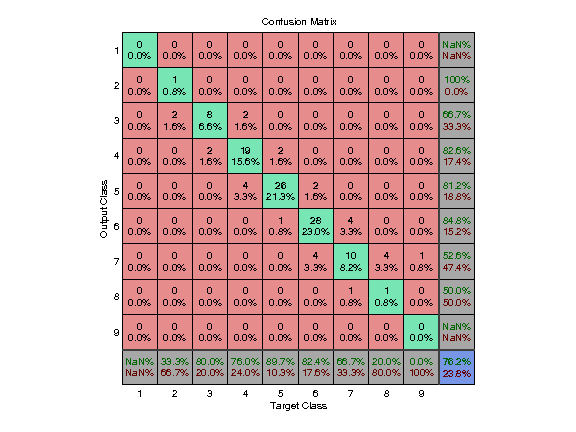
\includegraphics[scale=0.8]{../src/results/ordinal/ESL_mc1.png}
				\caption{Matriz de confusión. Conjunto de datos ESL. Clasificación ordinal.}
				\label{fig:ordesl}
			\end{figure}
			
			\subsubsection{Conjunto de datos Eucalyptus}
			
			En la Tabla \ref{tab:ordeuc} se muestran los resultados individuales de las 30 ejecuciones del algoritmo de regresión ordinal ORNNet mediante una red neuronal artificial ordinal para el conjunto de datos Eucalyptus, donde se muestra el número de ejecuciones, el CCR, el MAE, el número de neuronas en capa oculta calculado y el tiempo total de la ejecución.\\
			
			\begin{table}[!htbp]
				\centering
				\CSVtotabular{../src/results/ordinal/eucalyptus.csv}{l|r|r|r|r|r|r}{%
					\bfseries numIter &
					\bfseries CCR &
					\bfseries MAE &
					\bfseries NH &
					\bfseries CompTime\\\hline}{%
					\insertnumIter &
					\insertCCR &
					\insertMAE &
					\insertNH &
					\insertCompTime\\}{%
					\insertnumIter &
					\insertCCR &
					\insertMAE &
					\insertNH &
					\insertCompTime\\
					}
				\caption{Resultados individuales. Conjunto de datos Eucalyptus. Clasificación ordinal.}
				\label{tab:ordeuc}
			\end{table}
			
			La matriz de confusión para el mejor resultado del CCR obtenido de las 30 ejecuciones es la que se muestra en la Figura \ref{fig:ordeuc}.
			
			\begin{figure}[htbp]
				\centering
				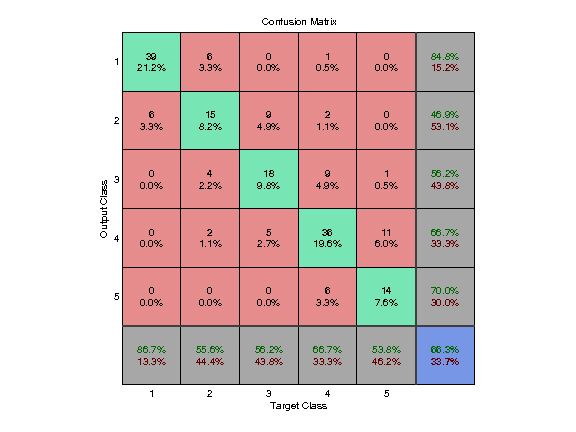
\includegraphics[scale=0.8]{../src/results/ordinal/eucalyptus_mc1.png}
				\caption{Matriz de confusión. Conjunto de datos Eucalyptus. Clasificación ordinal.}
				\label{fig:ordeuc}
			\end{figure}
			
			\subsubsection{Conjunto de datos LEV}
			
			En la Tabla \ref{tab:ordlev} se muestran los resultados individuales de las 30 ejecuciones del algoritmo de regresión ordinal ORNNet mediante una red neuronal artificial ordinal para el conjunto de datos LEV, donde se muestra el número de ejecuciones, el CCR, el MAE, el número de neuronas en capa oculta calculado y el tiempo total de la ejecución.\\
			
			\begin{table}[!htbp]
				\centering
				\CSVtotabular{../src/results/ordinal/LEV.csv}{l|r|r|r|r|r|r}{%
					\bfseries numIter &
					\bfseries CCR &
					\bfseries MAE &
					\bfseries NH &
					\bfseries CompTime\\\hline}{%
					\insertnumIter &
					\insertCCR &
					\insertMAE &
					\insertNH &
					\insertCompTime\\}{%
					\insertnumIter &
					\insertCCR &
					\insertMAE &
					\insertNH &
					\insertCompTime\\
					}
				\caption{Resultados individuales. Conjunto de datos LEV. Clasificación ordinal.}
				\label{tab:ordlev}
			\end{table}
			
			La matriz de confusión para el mejor resultado del CCR obtenido de las 30 ejecuciones es la que se muestra en la Figura \ref{fig:ordlev}.
			
			\begin{figure}[htbp]
				\centering
				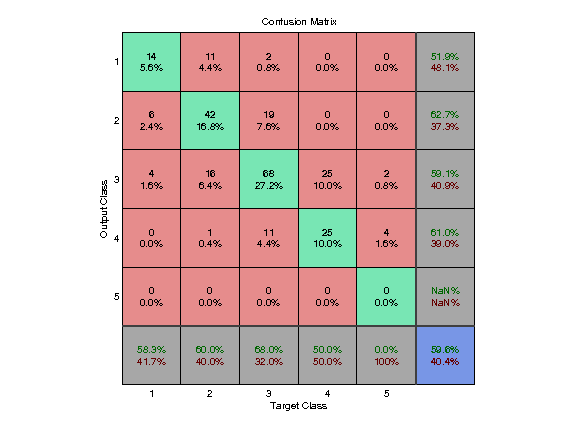
\includegraphics[scale=0.8]{../src/results/ordinal/LEV_mc1.png}
				\caption{Matriz de confusión. Conjunto de datos LEV. Clasificación ordinal.}
				\label{fig:ordlev}
			\end{figure}
			
			\subsubsection{Conjunto de datos New Thyroid}
			
			En la Tabla \ref{tab:ordnew} se muestran los resultados individuales de las 30 ejecuciones del algoritmo de regresión ordinal ORNNet mediante una red neuronal artificial ordinal para el conjunto de datos New Thyroid, donde se muestra el número de ejecuciones, el CCR, el MAE, el número de neuronas en capa oculta calculado y el tiempo total de la ejecución.\\
			
			\begin{table}[!htbp]
				\centering
				\CSVtotabular{../src/results/ordinal/newthyroid.csv}{l|r|r|r|r|r|r}{%
					\bfseries numIter &
					\bfseries CCR &
					\bfseries MAE &
					\bfseries NH &
					\bfseries CompTime\\\hline}{%
					\insertnumIter &
					\insertCCR &
					\insertMAE &
					\insertNH &
					\insertCompTime\\}{%
					\insertnumIter &
					\insertCCR &
					\insertMAE &
					\insertNH &
					\insertCompTime\\
					}
				\caption{Resultados individuales. Conjunto de datos New Thyroid. Clasificación ordinal.}
				\label{tab:ordnew}
			\end{table}
			
			La matriz de confusión para el mejor resultado del CCR obtenido de las 30 ejecuciones es la que se muestra en la Figura \ref{fig:ordnew}.
			
			\begin{figure}[htbp]
				\centering
				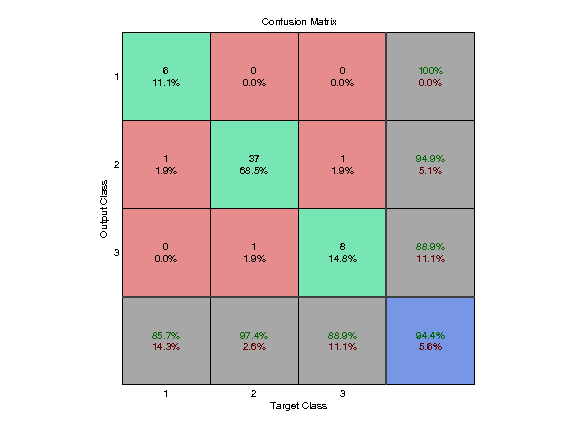
\includegraphics[scale=0.8]{../src/results/ordinal/newthyroid_mc1.png}
				\caption{Matriz de confusión. Conjunto de datos New Thyroid. Clasificación ordinal.}
				\label{fig:ordnew}
			\end{figure}
			
			\subsubsection{Conjunto de datos Pasture}
			
			En la Tabla \ref{tab:ordpas} se muestran los resultados individuales de las 30 ejecuciones del algoritmo de regresión ordinal ORNNet mediante una red neuronal artificial ordinal para el conjunto de datos Pasture, donde se muestra el número de ejecuciones, el CCR, el MAE, el número de neuronas en capa oculta calculado y el tiempo total de la ejecución.\\
			
			\begin{table}[!htbp]
				\centering
				\CSVtotabular{../src/results/ordinal/pasture.csv}{l|r|r|r|r|r|r}{%
					\bfseries numIter &
					\bfseries CCR &
					\bfseries MAE &
					\bfseries NH &
					\bfseries CompTime\\\hline}{%
					\insertnumIter &
					\insertCCR &
					\insertMAE &
					\insertNH &
					\insertCompTime\\}{%
					\insertnumIter &
					\insertCCR &
					\insertMAE &
					\insertNH &
					\insertCompTime\\
					}
				\caption{Resultados individuales. Conjunto de datos Pasture. Clasificación ordinal.}
				\label{tab:ordpas}
			\end{table}
			
			La matriz de confusión para el mejor resultado del CCR obtenido de las 30 ejecuciones es la que se muestra en la Figura \ref{fig:ordpas}.
			
			\begin{figure}[htbp]
				\centering
				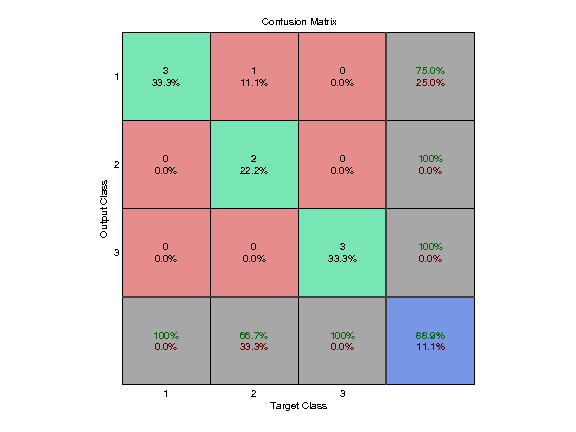
\includegraphics[scale=0.8]{../src/results/ordinal/pasture_mc1.png}
				\caption{Matriz de confusión. Conjunto de datos Pasture. Clasificación ordinal.}
				\label{fig:ordpas}
			\end{figure}
			
			\subsubsection{Conjunto de datos Squash Stored}
			
			En la Tabla \ref{tab:ordsqu} se muestran los resultados individuales de las 30 ejecuciones del algoritmo de regresión ordinal ORNNet mediante una red neuronal artificial ordinal para el conjunto de datos Squash Stored, donde se muestra el número de ejecuciones, el CCR, el MAE, el número de neuronas en capa oculta calculado y el tiempo total de la ejecución.\\
			
			\begin{table}[!htbp]
				\centering
				\CSVtotabular{../src/results/ordinal/squash-stored.csv}{l|r|r|r|r|r|r}{%
					\bfseries numIter &
					\bfseries CCR &
					\bfseries MAE &
					\bfseries NH &
					\bfseries CompTime\\\hline}{%
					\insertnumIter &
					\insertCCR &
					\insertMAE &
					\insertNH &
					\insertCompTime\\}{%
					\insertnumIter &
					\insertCCR &
					\insertMAE &
					\insertNH &
					\insertCompTime\\
					}
				\caption{Resultados individuales. Conjunto de datos Squash Stored. Clasificación ordinal.}
				\label{tab:ordsqu}
			\end{table}
			
			La matriz de confusión para el mejor resultado del CCR obtenido de las 30 ejecuciones es la que se muestra en la Figura \ref{fig:ordsqu}.
			
			\begin{figure}[htbp]
				\centering
				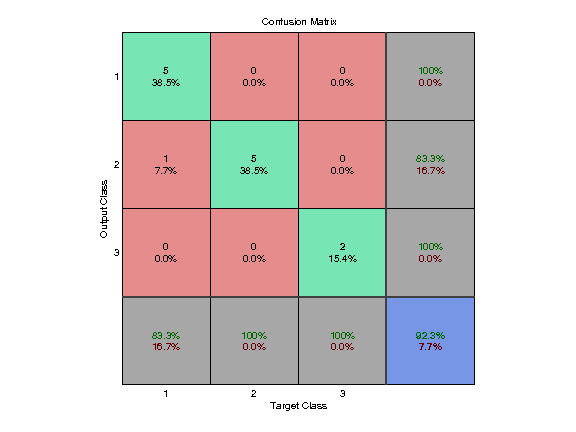
\includegraphics[scale=0.8]{../src/results/ordinal/squash-stored_mc1.png}
				\caption{Matriz de confusión. Conjunto de datos Squash Stored. Clasificación ordinal.}
				\label{fig:ordsqu}
			\end{figure}
			
			\subsubsection{Conjunto de datos Squash Unstored}
			
			En la Tabla \ref{tab:ordsqua} se muestran los resultados individuales de las 30 ejecuciones del algoritmo de regresión ordinal ORNNet mediante una red neuronal artificial ordinal para el conjunto de datos Squash Unstored, donde se muestra el número de ejecuciones, el CCR, el MAE, el número de neuronas en capa oculta calculado y el tiempo total de la ejecución.\\
			
			\begin{table}[!htbp]
				\centering
				\CSVtotabular{../src/results/ordinal/squash-unstored.csv}{l|r|r|r|r|r|r}{%
					\bfseries numIter &
					\bfseries CCR &
					\bfseries MAE &
					\bfseries NH &
					\bfseries CompTime\\\hline}{%
					\insertnumIter &
					\insertCCR &
					\insertMAE &
					\insertNH &
					\insertCompTime\\}{%
					\insertnumIter &
					\insertCCR &
					\insertMAE &
					\insertNH &
					\insertCompTime\\
					}
				\caption{Resultados individuales. Conjunto de datos Squash Unstored. Clasificación ordinal.}
				\label{tab:ordsqua}
			\end{table}
			
			La matriz de confusión para el mejor resultado del CCR obtenido de las 30 ejecuciones es la que se muestra en la Figura \ref{fig:ordsqua}.
			
			\begin{figure}[htbp]
				\centering
				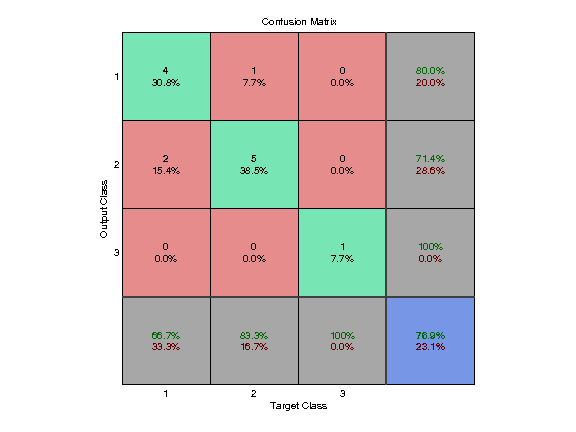
\includegraphics[scale=0.8]{../src/results/ordinal/squash-unstored_mc1.png}
				\caption{Matriz de confusión. Conjunto de datos Squash Unstored. Clasificación ordinal.}
				\label{fig:ordsqua}
			\end{figure}
			
			\subsubsection{Conjunto de datos SWD}
			
			En la Tabla \ref{tab:ordswd} se muestran los resultados individuales de las 30 ejecuciones del algoritmo de regresión ordinal ORNNet mediante una red neuronal artificial ordinal para el conjunto de datos SWD, donde se muestra el número de ejecuciones, el CCR, el MAE, el número de neuronas en capa oculta calculado y el tiempo total de la ejecución.\\
			
			\begin{table}[!htbp]
				\centering
				\CSVtotabular{../src/results/ordinal/SWD.csv}{l|r|r|r|r|r|r}{%
					\bfseries numIter &
					\bfseries CCR &
					\bfseries MAE &
					\bfseries NH &
					\bfseries CompTime\\\hline}{%
					\insertnumIter &
					\insertCCR &
					\insertMAE &
					\insertNH &
					\insertCompTime\\}{%
					\insertnumIter &
					\insertCCR &
					\insertMAE &
					\insertNH &
					\insertCompTime\\
					}
				\caption{Resultados individuales. Conjunto de datos SWD. Clasificación ordinal.}
				\label{tab:ordswd}
			\end{table}
			
			La matriz de confusión para el mejor resultado del CCR obtenido de las 30 ejecuciones es la que se muestra en la Figura \ref{fig:ordswd}.
			
			\begin{figure}[htbp]
				\centering
				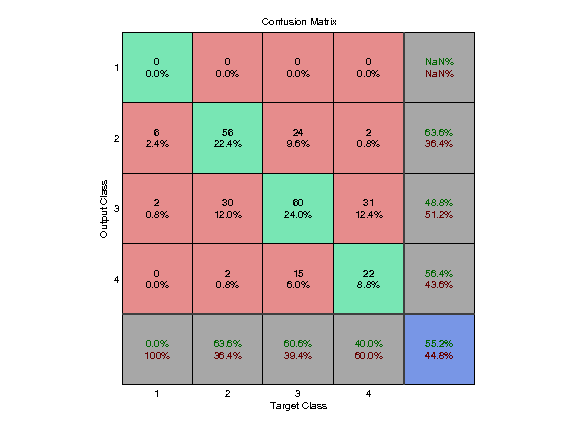
\includegraphics[scale=0.8]{../src/results/ordinal/SWD_mc1.png}
				\caption{Matriz de confusión. Conjunto de datos SWD. Clasificación ordinal.}
				\label{fig:ordswd}
			\end{figure}
			
			\subsubsection{Conjunto de datos TAE}
			
			En la Tabla \ref{tab:ordtae} se muestran los resultados individuales de las 30 ejecuciones del algoritmo de regresión ordinal ORNNet mediante una red neuronal artificial ordinal para el conjunto de datos TAE, donde se muestra el número de ejecuciones, el CCR, el MAE, el número de neuronas en capa oculta calculado y el tiempo total de la ejecución.\\
			
			\begin{table}[!htbp]
				\centering
				\CSVtotabular{../src/results/ordinal/tae.csv}{l|r|r|r|r|r|r}{%
					\bfseries numIter &
					\bfseries CCR &
					\bfseries MAE &
					\bfseries NH &
					\bfseries CompTime\\\hline}{%
					\insertnumIter &
					\insertCCR &
					\insertMAE &
					\insertNH &
					\insertCompTime\\}{%
					\insertnumIter &
					\insertCCR &
					\insertMAE &
					\insertNH &
					\insertCompTime\\
					}
				\caption{Resultados individuales. Conjunto de datos TAE. Clasificación ordinal.}
				\label{tab:ordtae}
			\end{table}
			
			La matriz de confusión para el mejor resultado del CCR obtenido de las 30 ejecuciones es la que se muestra en la Figura \ref{fig:ordtae}.
			
			\begin{figure}[htbp]
				\centering
				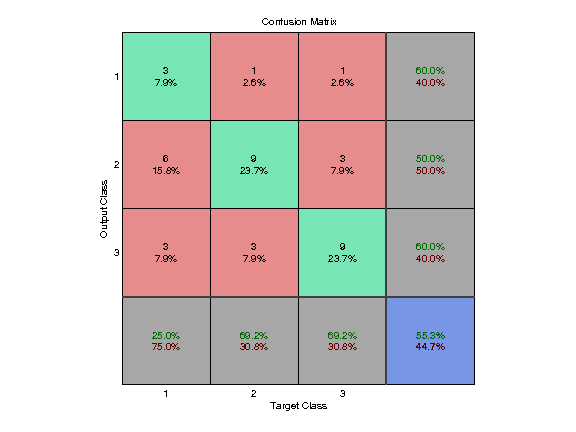
\includegraphics[scale=0.8]{../src/results/ordinal/tae_mc1.png}
				\caption{Matriz de confusión. Conjunto de datos TAE. Clasificación ordinal.}
				\label{fig:ordtae}
			\end{figure}
			
			\subsubsection{Conjunto de datos Thyroid}
			
			En la Tabla \ref{tab:ordthy} se muestran los resultados individuales de las 30 ejecuciones del algoritmo de regresión ordinal ORNNet mediante una red neuronal artificial ordinal para el conjunto de datos Thyroid, donde se muestra el número de ejecuciones, el CCR, el MAE, el número de neuronas en capa oculta calculado y el tiempo total de la ejecución.\\
			
			\begin{table}[!htbp]
				\centering
				\CSVtotabular{../src/results/ordinal/thyroid.csv}{l|r|r|r|r|r|r}{%
					\bfseries numIter &
					\bfseries CCR &
					\bfseries MAE &
					\bfseries NH &
					\bfseries CompTime\\\hline}{%
					\insertnumIter &
					\insertCCR &
					\insertMAE &
					\insertNH &
					\insertCompTime\\}{%
					\insertnumIter &
					\insertCCR &
					\insertMAE &
					\insertNH &
					\insertCompTime\\
					}
				\caption{Resultados individuales. Conjunto de datos Thyroid. Clasificación ordinal.}
				\label{tab:ordthy}
			\end{table}
			
			La matriz de confusión para el mejor resultado del CCR obtenido de las 30 ejecuciones es la que se muestra en la Figura \ref{fig:ordthy}.
			
			\begin{figure}[htbp]
				\centering
				\includegraphics[scale=0.8]{../src/results/ordinal/thyroid_mc1.png}
				\caption{Matriz de confusión. Conjunto de datos Thyroid. Clasificación ordinal.}
				\label{fig:ordthy}
			\end{figure}
			
			\subsubsection{Conjunto de datos Wine Quality Red}
			
			En la Tabla \ref{tab:ordred} se muestran los resultados individuales de las 30 ejecuciones del algoritmo de regresión ordinal ORNNet mediante una red neuronal artificial ordinal para el conjunto de datos Wine Quality Red, donde se muestra el número de ejecuciones, el CCR, el MAE, el número de neuronas en capa oculta calculado y el tiempo total de la ejecución.\\
			
			\begin{table}[!htbp]
				\centering
				\CSVtotabular{../src/results/ordinal/winequality-red.csv}{l|r|r|r|r|r|r}{%
					\bfseries numIter &
					\bfseries CCR &
					\bfseries MAE &
					\bfseries NH &
					\bfseries CompTime\\\hline}{%
					\insertnumIter &
					\insertCCR &
					\insertMAE &
					\insertNH &
					\insertCompTime\\}{%
					\insertnumIter &
					\insertCCR &
					\insertMAE &
					\insertNH &
					\insertCompTime\\
					}
				\caption{Resultados individuales. Conjunto de datos Wine Quality Red. Clasificación ordinal.}
				\label{tab:ordred}
			\end{table}
			
			La matriz de confusión para el mejor resultado del CCR obtenido de las 30 ejecuciones es la que se muestra en la Figura \ref{fig:ordred}.
			
			\begin{figure}[htbp]
				\centering
				\includegraphics[scale=0.8]{../src/results/ordinal/winequality-red_mc1.png}
				\caption{Matriz de confusión. Conjunto de datos Wine Quality Red. Clasificación ordinal.}
				\label{fig:ordred}
			\end{figure}
			
			\subsubsection{Conjunto de datos Wine Quality White}
			
			En la Tabla \ref{tab:ordwhi} se muestran los resultados individuales de las 30 ejecuciones del algoritmo de regresión ordinal ORNNet mediante una red neuronal artificial ordinal para el conjunto de datos Wine Quality White, donde se muestra el número de ejecuciones, el CCR, el MAE, el número de neuronas en capa oculta calculado y el tiempo total de la ejecución.\\
			
			\begin{table}[!htbp]
				\centering
				\CSVtotabular{../src/results/ordinal/winequality-white.csv}{l|r|r|r|r|r|r}{%
					\bfseries numIter &
					\bfseries CCR &
					\bfseries MAE &
					\bfseries NH &
					\bfseries CompTime\\\hline}{%
					\insertnumIter &
					\insertCCR &
					\insertMAE &
					\insertNH &
					\insertCompTime\\}{%
					\insertnumIter &
					\insertCCR &
					\insertMAE &
					\insertNH &
					\insertCompTime\\
					}
				\caption{Resultados individuales. Conjunto de datos Wine Quality White. Clasificación ordinal.}
				\label{tab:ordwhi}
			\end{table}
			
			La matriz de confusión para el mejor resultado del CCR obtenido de las 30 ejecuciones es la que se muestra en la Figura \ref{fig:ordwhi}.
			
			\begin{figure}[htbp]
				\centering
				\includegraphics[scale=0.8]{../src/results/ordinal/winequality-white_mc1.png}
				\caption{Matriz de confusión. Conjunto de datos Wine Quality White. Clasificación ordinal.}
				\label{fig:ordwhi}
			\end{figure}
			
	\section{Resultados generales}
		
		Estos resultados son los obtenidos a partir de los resultados individuales, es decir, de cada uno de los conjuntos de datos se ha realizado la media y la desviación típica del CCR, el MAE y el NH.\\
		
		A partir de estos datos se podrá observar como de buenos son los resultados para una posterior comparativa.
		
		\subsection{Clasificación Nominal}
		
			La Tabla \ref{tab:gennom} muestra los resultados generales para los conjuntos de datos aplicando la clasificación nominal para la creación de la red neuronal y el entrenamiento y simulación.\\
		
			\begin{table}[!htbp]
				\centering
				\CSVtotabular{../src/results/nominal/general.csv}{l|r|r|r|r|r|r}{%
					\bfseries dataset &
					\bfseries CCRMean &
					\bfseries CCRSD &
					\bfseries MAEMean &
					\bfseries MAESD &
					\bfseries NHMean &
					\bfseries NHSD\\\hline}{%
					\insertdataset &
					\insertbyname{CCRMean} &
					\insertCCRSD &
					\insertMAEMean &
					\insertMAESD &
					\insertNHMean &
					\insertNHSD\\}{%
					\insertdataset &
					\insertbyname{CCRMean} &
					\insertCCRSD &
					\insertMAEMean &
					\insertMAESD &
					\insertNHMean &
					\insertNHSD\\
					}
				\caption{Resultados generales. Clasificación nominal.}
				\label{tab:gennom}
			\end{table}
		
		\subsection{Clasificación Ordinal}
		
			La Tabla \ref{tab:genord} muestra los resultados generales para los conjuntos de datos aplicando la clasificación ordinal para la creación de la red neuronal y el entrenamiento y simulación.
	
			\begin{table}[!htbp]
				\centering
				\CSVtotabular{../src/results/ordinal/general.csv}{l|r|r|r|r|r|r}{%
					\bfseries dataset &
					\bfseries CCRMean &
					\bfseries CCRSD &
					\bfseries MAEMean &
					\bfseries MAESD &
					\bfseries NHMean &
					\bfseries NHSD\\\hline}{%
					\insertdataset &
					\insertbyname{CCRMean} &
					\insertCCRSD &
					\insertMAEMean &
					\insertMAESD &
					\insertNHMean &
					\insertNHSD\\}{%
					\insertdataset &
					\insertbyname{CCRMean} &
					\insertCCRSD &
					\insertMAEMean &
					\insertMAESD &
					\insertNHMean &
					\insertNHSD\\
					}
				\caption{Resultados generales. Clasificación ordinal.}
				\label{tab:genord}
			\end{table}
	
	\section{Comparativa entre los resultados}
	
		En esta sección se hará un estudio comparativo entre las dos metodologías empleadas, nominal y ordinal, y de las cuales se podrán obtener las conclusiones en un capítulo posterior.\\
		
		Se hará una comparación entre los resultados generales de cada uno de las clasificaciones, observando y resaltando en cada caso cual ha sido mejor o peor para los conjuntos de datos evaluados. Para la comparativa entre los resultados obtenidos nos fijaremos en los valores medios del \textit{CCR} y del \textit{MAE}.\\
		
		Como se puede observar en la Tabla \ref{tab:comp}, los resultados obtenidos por el algoritmo ordinal ORNNet son mejores que para el algoritmo nominal, puesto que en 12 de los conjuntos de datos el \textit{CCR} es mayor que los resultados del algoritmo nominal y en 15 es menor el valor del \textit{MAE} para el ordinal. Además, en 11 la desviación típica es menor para el \textit{CCR} utilizando la clasificación ordinal frente a la nominal y en 14 también es menor la desviación típica para el \textit{MAE} utilizando la clasificación ordinal.
		
		\newpage{\thispagestyle{empty}}
		
		\begin{sidewaystable}[htbp]
			\centering
			\begin{tabular}{l|r|r|r|r|r|r|r|r}
				\cline{2-9}
				& \multicolumn{4}{c|}{\textbf{Nominal}} & \multicolumn{4}{c|}{\textbf{Ordinal}} \\
				\hline \textbf{dataset} & \textbf{CCRMean} & \textbf{CCRSD} & \textbf{MAEMean} & \textbf{MAESD} & \textbf{CCRMean} & \textbf{CCRSD} & \textbf{MAEMean} & \textbf{MAESD} \\ 
				\hline ERA & \cellcolor{myred} 0.249333 & 0.026623 & \cellcolor{myred} 1.360267 & 0.150086 & \cellcolor{mygreen} 0.267600 & 0.025415 & \cellcolor{mygreen} 1.240133 & 0.081750\\ 
				ESL & \cellcolor{myred} 0.694536 & 0.028794 & \cellcolor{myred} 0.329235 & 0.031200 & \cellcolor{mygreen} 0.714481 & 0.041744 & \cellcolor{mygreen} 0.302732 & 0.044685\\ 
				LEV & \cellcolor{myred} 0.598933 & 0.033564 & \cellcolor{myred} 0.431067 & 0.037665 & \cellcolor{mygreen} 0.607067 & 0.040936 & \cellcolor{mygreen} 0.419333 & 0.043490\\ 
				SWD & \cellcolor{myred} 0.561733 & 0.031839 & \cellcolor{myred} 0.467867 & 0.037294 & \cellcolor{mygreen} 0.567733 & 0.027270 & \cellcolor{mygreen} 0.451467 & 0.033855\\ 
				automobile & \cellcolor{myred} 0.600000 & 0.089548 & \cellcolor{myred} 0.580128 & 0.144536 & \cellcolor{mygreen} 0.641667 & 0.085480 & \cellcolor{mygreen} 0.443590 & 0.117023\\ 
				balance & \cellcolor{myred} 0.928662 & 0.026469 & \cellcolor{myred} 0.083864 & 0.034446 & \cellcolor{mygreen} 0.963907 & 0.018041 & \cellcolor{mygreen} 0.039066 & 0.019843\\ 
				bondrate & \cellcolor{myred} 0.560000 & 0.077509 & \cellcolor{myred} 0.606667 & 0.124229 & \cellcolor{mygreen} 0.568889 & 0.083475 & \cellcolor{mygreen} 0.584444 & 0.093765\\ 
				car & \cellcolor{mygreen} 0.977701 & 0.010900 & \cellcolor{mygreen} 0.025617 & 0.012634 & \cellcolor{myred} 0.968827 & 0.010955 & \cellcolor{myred} 0.031327 & 0.011039\\ 
				contact-lenses & \cellcolor{mygreen} 0.661111 & 0.202869 & \cellcolor{myred} 0.500000 & 0.327536 & \cellcolor{myred} 0.650000 & 0.153815 & \cellcolor{mygreen} 0.427778 & 0.184055\\ 
				depresion & \cellcolor{mygreen} 0.653283 & 0.192474 & \cellcolor{myred} 0.509091 & 0.316757 & \cellcolor{myred} 0.647475 & 0.149711 & \cellcolor{mygreen} 0.430808 & 0.179999\\ 
				eucalyptus & \cellcolor{myred} 0.599638 & 0.036704 & \cellcolor{myred} 0.476993 & 0.055290 & \cellcolor{mygreen} 0.650906 & 0.035615 & \cellcolor{mygreen} 0.385145 & 0.032663\\ 
				newthyroid & \cellcolor{myred} 0.956790 & 0.032014 & \cellcolor{myred} 0.043210 & 0.032014 & \cellcolor{mygreen} 0.964198 & 0.024284 & \cellcolor{mygreen} 0.035802 & 0.024284\\ 
				pasture & \cellcolor{mygreen} 0.722222 & 0.119421 & \cellcolor{mygreen} 0.311111 & 0.138101 & \cellcolor{myred} 0.648148 & 0.127468 & \cellcolor{myred} 0.351852 & 0.127468\\ 
				squash-stored & \cellcolor{myred} 0.656410 & 0.139567 & \cellcolor{myred} 0.366667 & 0.154750 & \cellcolor{mygreen} 0.661538 & 0.115340 & \cellcolor{mygreen} 0.353846 & 0.125507\\ 
				squash-unstored & \cellcolor{mygreen} 0.669231 & 0.131151 & \cellcolor{mygreen} 0.330769 & 0.131151 & \cellcolor{myred} 0.653846 & 0.156150 & \cellcolor{myred} 0.348718 & 0.160001\\ 
				tae & \cellcolor{myred} 0.414912 & 0.085952 & \cellcolor{myred} 0.764912 & 0.145938 & \cellcolor{mygreen} 0.441228 & 0.072047 & \cellcolor{mygreen} 0.648246 & 0.068233\\ 
				thyroid & \cellcolor{mygreen} 0.944630 & 0.008216 & \cellcolor{mygreen} 0.101574 & 0.015156 & \cellcolor{myred} 0.929426 & 0.006682 & \cellcolor{myred} 0.118352 & 0.013353\\ 
				winequality-red & \cellcolor{myred} 0.578250 & 0.016856 & \cellcolor{myred} 0.459833 & 0.020128 & \cellcolor{mygreen} 0.580833 & 0.020754 & \cellcolor{mygreen} 0.449917 & 0.022993\\ 
				winequality-white & \cellcolor{mygreen} 0.543728 & 0.010689 & \cellcolor{myred} 0.515374 & 0.009745 & \cellcolor{myred} 0.540789 & 0.012448 & \cellcolor{mygreen} 0.508408 & 0.012904\\
				\hline
			\end{tabular}
			\caption{Comparativa entre resultados generales.}
			\label{tab:comp}
		\end{sidewaystable}

	\chapter{Conclusiones y Futuras Mejoras}
	
	Una vez concluido el desarrollo y la experimentación del proyecto, se realizará una exposición de las conclusiones que se han extraído. Estas conclusiones irán en relación con los objetivos planteados al principio del desarrollo especificados en el Capítulo de Objetivos y con los resultados obtenidos durante la fase de experimentación.
	
	\section{Conclusiones}
		
		En esta sección se va a considerar cuales de los objetivos se han alcanzado en la realización del Proyecto. Una vez finalizado el desarrollo de la implementación del algoritmo de regresión ordinal para redes neuronales y la aplicación gráfica, se puede concretar que se han cumplido los requisitos especificados al comienzo del Proyecto.\\
		
		Los objetivos alcanzados han sido los siguientes:
		
		\begin{itemize}
			\item Se ha desarrollado la implementación del algoritmo propuesto de forma teórica para regresión ordinal basado en redes neuronales artificiales.
			\item Se ha realizado una comparativa de los resultados obtenidos basado en efectividad de la clasificación obtenida por el algoritmo nominal y el nuevo algoritmo basado en la ordinalidad de las clases.
			\item Se ha desarrollado una herramienta software para el tratado y la obtención de resultados a partir de un conjunto de datos, aplicando el algoritmo implementado basado en redes neuronales y haciendo uso del toolbox de Matlab, \textit{nnet}. Dicha herramienta ha sido implementada optimizando al máximo tanto la precisión de los modelos generados como el tiempo de computación necesario para obtener los resultados y que es algo muy importante en algoritmos de este estilo.
			\item Se ha modularizado todas los módulos y funciones para que tenga una compatibilidad completa con el toolbox nnet de Matlab.
			\item Se ha realizado un diseño experimental para cada uno de los problemas considerados, ajustando los parámetros de los experimentos y extrayendo las conclusiones pertinentes. Los modelos obtenidos como solución a dichos problemas han obtenido unos resultados muy buenos en clasificación, mejorando en un porcentaje variable para cada caso específico los resultados que hasta ahora se habían obtenido con modelos de clasificación nominal.
		\end{itemize}
		
		Por todos estos motivos, considerando que el proyecto que se ha desarrollado ha conseguido abarcar todas las metas que se propusieron al inicio del mismo, es un orgullo y una satisfacción haber aportado al grupo de investigación AYRNA, en sus estudios sobre aprendizaje e inteligencia artificial con ayuda de las redes neuronales artificiales, la implementación y comprobación del algoritmo desarrollado de forma teórica y la aportación de una interfaz gráfica completa y compatible con la librería de Matlab.
		
	\section{Futuras Mejoras}
		
		En esta sección se expondrán varias ideas con posibles mejoras a alcanzar en futuras ampliaciones del trabajo desarrollado.\\
		
		Como se ha expuesto a lo largo del desarrollo del presente proyecto, el objetivo principal era el desarrollo de la implementación del algoritmo de regresión ordinal y la comprobación de la efectividad del mismo en comparación con el método nominal.\\
		
		Dicho esto, se podría ver como una posible mejora del proyecto el estudio continuo de nuevos algoritmos basados en regresión ordinal y a partir de estos la nueva implementación de otro algoritmo que mejorase la efectividad de los resultados.\\
		
		Otra posible mejora sería el aumento de la funcionalidad de la herramienta software, por ejemplo, añadiendo la funcionalidad para la realización del método nominal o algún otro método basado en redes neuronales.\\
		
		Por último, otra posible mejora que podría realizarse es la adaptación, en alguno de los sentidos, al toolbox nnet de Matlab del resto de algoritmos o desarrollos que el grupo de investigación AYRNA tiene de proyectos o estudios anteriores basados en redes neuronales artificiales, completando así dicho paquete de software computacionalmente muy potente.

	
	%BIBLIOGRAFIA
	\clearpage
\addcontentsline{toc}{chapter}{Bibliografía}

\begin{thebibliography}{99}
	\bibitem{Bishop} Bishop C.M., ``Pattern recognition and machine learning". Singapur, Springer, 676 p, ISBN-10: 0-387-31073-8.
	\bibitem{Ch05} W. Chu and S.S. Keerthi, ``New Approaches to Support Vector Ordinal Regression". Proc. 22nd Int. Conf. Machine Learning (ICML ’05), pp. 145-152, 2005.
	\bibitem{Lin07} L. Lin and H.-T. Lin, ``Ordinal Regression by Extended Binary Classification". Advances in Neural Infor. Processing Systems, vol. 19, pp. 865-872, MIT Press, 2007.
	\bibitem{Mcc80} McCullagh, ``P. Regression models for ordinal data". Journal of the Royal Statistical Society, Series B (Methodological), 42, 109–142, 1980.
	\bibitem{Sh03} Shashua and A. Levin, ``Ranking with Large Margin Principle: Two Approaches", Advances in Neural Inform. Processing Systems, vol. 15, 961-968, MIT Press, 2003.
	\bibitem{RPROP} Riedmiller, Martin. ``RPROP - Descriptión and Implmentation Details". University of Karlsruhe. Technical Report, 1994.
	\bibitem{iRPROP+} Igel, Christian; Hüsken, Michael. ``Empirical evaluation of the improved RPROP learning algorithms". Institut für Neuroinformatik, Ruhr-Universität Bochum. Germany, 2001.
	\bibitem{Matlab} ``MATLAB version 2010a for Ubuntu". Natick, Massachusetts. The MathWorks Inc., 2010.
	\bibitem{Matlab_ref} ``Documentación oficial de MATLAB". Natick, Massachusetts. The MathWorks Inc., 2010. Enlace: \url{http://www.mathworks.com/help/techdoc/}
	\bibitem{Matlab_nnet} ``Documentación oficial de MATLAB para el Toolbox NNET". Natick, Massachusetts. The MathWorks Inc., 2010. Enlace: \url{http://www.mathworks.com/help/toolbox/nnet/}
	\bibitem{Matlab_gui} ``Documentación oficial de MATLAB para creación de GUIs (Graphical User Interfaces)". Natick, Massachusetts. The MathWorks Inc., 2010. Enlace: \url{http://www.mathworks.com/help/techdoc/creating_guis/bqz79mu.html}
	\bibitem{UML} G. Booch, J. Rumbaugh, I. Jacobson, ``El lenguaje Unificado de Modelado". Ed. Addison Wesley Iberoamericana. Madrid, 1999.
\end{thebibliography}
	
	%APENDICES
	\appendix
	\chapter{Manual de usuario}
	
	Este apéndice constituye el manual de usuario del producto software desarrollado por el presente proyecto fin de carrera e incluye la información necesaria para su ejecución.
	
	\section{Instalación y desinstalación}
		
		En esta sección se realizará una explicación de cómo se podrá instalar y desinstalar la nueva funcionalidad del toolbox \textit{nnet} añadida por las nuevas funciones y la aplicación gráfica.
		
		\subsection{Instalación}
		
			Para la instalación se requerirá un descompresor, ya que todo el código fuente del toolbox se encontrará en archivo comprimido .zip como se muestra en la Figura \ref{fig:arc_com}.\\
			
			\begin{figure}[htbp]
				\centering
				\includegraphics[scale=1]{img/arc_com.png}
				\caption{Instalación. Archivo del código fuente comprimido.}
				\label{fig:arc_com}
			\end{figure}
			
			Al descomprimir el archivo comprimido se quedará la carpeta con el código fuente, como se muestra en la Figura \ref{fig:car_src}, lista para poder añadirla al \textit{path} de Matlab.\\
			
			\begin{figure}[htbp]
				\centering
				\includegraphics[scale=1]{img/car_src.png}
				\caption{Instalación. Carpeta del código fuente.}
				\label{fig:car_src}
			\end{figure}
			
			Para añadir el código al \textit{path} de Matlab habrá que seguir los siguientes pasos:\\
			
			Primero seleccione del menú \textit{File} y pulse sobre la opción \textit{Set Path} tal y como se muestra en la Figura \ref{fig:menu}.\\
			
			\begin{figure}[htbp]
				\centering
				\includegraphics[scale=0.6]{img/menu.png}
				\caption{Instalación. Menú File.}
				\label{fig:menu}
			\end{figure}
			
			Aparecerá una pantalla como la que se muestra en la Figura \ref{fig:path}. En esta pantalla deberá seleccionar la opción \textit{Add with Subfolders}.\\
			
			\begin{figure}[htbp]
				\centering
				\includegraphics[scale=0.4]{img/path.png}
				\caption{Instalación. Añadir al Path.}
				\label{fig:path}
			\end{figure}
			
			En este momento aparecerá un cuadro de diálogo como el que se muestra en la Figura \ref{fig:dialog} en el que deberá seleccionar la carpeta que se ha descomprimido y que contiene todo el código fuente.\\
			
			\begin{figure}[htbp]
				\centering
				\includegraphics[scale=0.6]{img/dialog.png}
				\caption{Instalación. Cuadro de diálogo.}
				\label{fig:dialog}
			\end{figure}
			
			Al pulsar \textit{OK} del cuadro de diálogo se añadirá todo el contenido al \textit{Path} de Matlab. En este momento habrá que pulsar sobre el botón \textit{Save} y luego en \textit{Close}, con lo que ya se podrá llamar a cualquiera de las funciones del nuevo \textit{toolbox} como a cualquier otra función propia de Matlab.
		
		\subsection{Desinstalación}
		
			Para la desinstalación de la nueva funcionalidad del \textit{toolbox} para Matlab sólo habrá que realizar un paso. Como se puede observar en la Figura \ref{fig:path2}, el \textit{path} contendrá el árbol de contenidos del \textit{toolbox}, con lo que habrá que seleccionar todos los elementos y seguidamente pulsar sobre el botón \textit{Remove}. Una vez eliminado deberá pulsar sobre el botón \textit{Save} y seguidamente sobre \textit{Close} y ya estará todo desinstalado.
			
			\begin{figure}[htbp]
				\centering
				\includegraphics[scale=0.4]{img/path.png}
				\caption{Desinstalación. Eliminación de contenido del Path.}
				\label{fig:path2}
			\end{figure}
		
	\section{Uso de la aplicación}
	
		En esta sección se expondrá un ejemplo de la aplicación para que cualquiera pueda usarla. Se explicará detalladamente cada pantalla que proporciona la aplicación mostrando además una imagen de la misma.\\
		
		La primera pantalla que se verá cuando se inicia la aplicación será la pantalla inicial de bienvenida, que se muestra en la Figura \ref{fig:int01}. En esta pantalla se puede observar los siguientes elementos: una barra en la parte superior con el nombre de la aplicación ``nntool", seguidamente se muestra una cabecera en la que se ve el saludo de bienvenida a la aplicación junto a los escudos de la Universidad de Córdoba y de Ingeniería Informática. Después se muestran dos paneles, uno con información general sobre el tema que se trata y otro con información específica sobre redes neuronales ordinales. Dos de los botones que contiene esta pantalla y que contendrán el resto a partir de ahora a excepción de la última pantalla son los botones para pasar a la siguiente pantalla (Next) y para cancelar la aplicación y salirse (Cancel).\\
		
		\begin{figure}[htbp]
			\centering
			\includegraphics[scale=0.5]{interfaz/interface01.png}
			\caption{Interfaz gráfica. Pantalla de bienvenida.}
			\label{fig:int01}
		\end{figure}
		
		Al pulsar el botón siguiente (Next) se pasará a la siguiente pantalla, la pantalla de obtención de datos, la cual muestra dos paneles, uno para cargar los datos del conjunto de entrenamiento y otro para cargar los datos del conjunto de test. Estos paneles constan de un menú popup en el que se mostrarán de cada conjunto los datos de entrada (Inputs) y los datos objetivos (Targets).\\
		
		\begin{figure}[htbp]
			\centering
			\includegraphics[scale=0.5]{interfaz/interface02.png}
			\caption{Interfaz gráfica. Pantalla de carga de datos.}
			\label{fig:int02}
		\end{figure}
		
		Si se intenta pasar a la siguiente pantalla pulsando directamente el botón siguiente (Next) sin haber cargado los conjuntos de datos, se mostrará un mensaje de advertencia como el que se muestra en la Figura \ref{fig:int02-1}.\\
		
		\begin{figure}[htbp]
			\centering
			\includegraphics[scale=1]{interfaz/interface02-1.png}
			\caption{Interfaz gráfica. Aviso de falta de carga de datos.}
			\label{fig:int02-1}
		\end{figure}
		
		En caso de que no haya datos cargados previamente, habrá que pulsar alguno de los botones para abrir un cuadro de diálogo y de este modo poder cargar un conjunto de datos desde un par de ficheros (train y test). Las Figuras de la \ref{fig:int03} a la \ref{fig:int07} muestran como se puede cargar un par de ficheros de un conjunto de datos paso a paso.\\
		
		\begin{figure}[htbp]
			\centering
			\includegraphics[scale=0.6]{interfaz/interface03.png}
			\caption{Interfaz gráfica. Carga de datos.}
			\label{fig:int03}
		\end{figure}
		
		\begin{figure}[htbp]
			\centering
			\includegraphics[scale=0.6]{interfaz/interface04.png}
			\caption{Interfaz gráfica. Selección de la carpeta datasets.}
			\label{fig:int04}
		\end{figure}
		
		\begin{figure}[htbp]
			\centering
			\includegraphics[scale=0.6]{interfaz/interface05.png}
			\caption{Interfaz gráfica. Selección de la carpeta 10-holdout.}
			\label{fig:int05}
		\end{figure}
		
		\begin{figure}[htbp]
			\centering
			\includegraphics[scale=0.6]{interfaz/interface06.png}
			\caption{Interfaz gráfica. Selección del fichero de entrenamiento.}
			\label{fig:int06}
		\end{figure}
		
		\begin{figure}[htbp]
			\centering
			\includegraphics[scale=0.6]{interfaz/interface07.png}
			\caption{Interfaz gráfica. Selección del fichero de test.}
			\label{fig:int07}
		\end{figure}
		
		Una vez seleccionados los datos se mostrará una breve información sobre las dimensiones de los conjuntos de datos en el panel de información de la derecha. La Figura \ref{fig:int08} muestra dicha pantalla con la información del ejemplo cargado. \\
		
		\begin{figure}[htbp]
			\centering
			\includegraphics[scale=0.5]{interfaz/interface08.png}
			\caption{Interfaz gráfica. Datos cargados.}
			\label{fig:int08}
		\end{figure}
		
		Si al intentar cargar los datos se produce una equivocación en el fichero de datos o se intenta cargar un fichero con una extensión incorrecta, se mostrará un aviso para que se carguen de nuevo los datos correctos y no se hará nada. Si todo el proceso se ha seguido correctamente se podrá pulsar el botón de siguiente (Next) o de atrás (Back) para navegar entre pantallas.\\
		
		Una vez pulsado el botón para pasar a la siguiente pantalla (Next), se pasará a la pantalla de configuración de la red neuronal ordinal. Esta pantalla está constituida por dos paneles, uno para la configuración de la red propiamente en la parte izquierda y otro que muestra la información de las acciones disponibles en la parte derecha. La Figura \ref{fig:int09} muestra dicha pantalla.\\
		
		\begin{figure}[htbp]
			\centering
			\includegraphics[scale=0.5]{interfaz/interface09.png}
			\caption{Interfaz gráfica. Pantalla de configuración de la red neuronal.}
			\label{fig:int09}
		\end{figure}
		
		En esta pantalla existen dos posibilidades para la configuración de la red neuronal ordinal, la posibilidad de realizar un K-fold cross-validation de los conjuntos de entrenamiento y test para obtener el valor del número de neuronas óptimo de la capa oculta o especificarlo manualmente (20 por defecto). También se tendrá que especificar en ambos casos la función de transferencia a usar, que podrá ser \textit{logsig} o \textit{tansig}. Las Figuras \ref{fig:int10} y \ref{fig:int11} muestran dichas pantallas.\\
		
		\begin{figure}[htbp]
			\centering
			\includegraphics[scale=0.5]{interfaz/interface10.png}
			\caption{Interfaz gráfica. Opción manual de configuración de la red neuronal.}
			\label{fig:int10}
		\end{figure}
		
		\begin{figure}[htbp]
			\centering
			\includegraphics[scale=1]{interfaz/interface11.png}
			\caption{Interfaz gráfica. Opción de función de transferencia.}
			\label{fig:int11}
		\end{figure}
		
		Si se elige la opción de realizar un K-fold, se podrá especificar el valor de \textit{k} (10 por defecto). Una vez seleccionado el valor de \textit{k} habrá que pulsar el botón de K-fold para realizar el proceso. Si se intenta pasar directamente a la siguiente pantalla sin pulsar dicho botón, se mostrará un aviso para que se pulse el botón y se pueda realizar el K-fold. La Figura \ref{fig:int12} muestra dicha pantalla y la Figura \ref{fig:int12-1} muestra el aviso.\\
		
		\begin{figure}[htbp]
			\centering
			\includegraphics[scale=0.5]{interfaz/interface12.png}
			\caption{Interfaz gráfica. Opción para realizar un K-fold.}
			\label{fig:int12}
		\end{figure}
		
		\begin{figure}[htbp]
			\centering
			\includegraphics[scale=1]{interfaz/interface12-1.png}
			\caption{Interfaz gráfica. Aviso de la opción K-fold.}
			\label{fig:int12-1}
		\end{figure}
		
		Mientras se realiza el K-fold cross-validation se presentará un mensaje de espera para informar que el proceso está activo. Una vez terminado el proceso, se cerrará el mensaje y se podrá pasar a la siguiente pantalla.\\
		
		\begin{figure}[htbp]
			\centering
			\includegraphics[scale=1]{interfaz/interface12-2.png}
			\caption{Interfaz gráfica. Barra de espera de la opción K-fold.}
			\label{fig:int12-2}
		\end{figure}
		
		Al pasar a la siguiente pantalla, que es la pantalla de entrenamiento, se mostrarán dos nuevos paneles. El primer panel mostrará el botón para realizar el entrenamiento de la red (Train). La Figura \ref{fig:int13} muestra dicha pantalla.\\
		
		\begin{figure}[htbp]
			\centering
			\includegraphics[scale=0.5]{interfaz/interface13.png}
			\caption{Interfaz gráfica. Pantalla de entrenamiento.}
			\label{fig:int13}
		\end{figure}
		
		El segundo panel, en cambio, mostrará los resultados del proceso de entrenamiento y simulación. Adicionalmente, en esta pantalla se añade un nuevo botón para poder ver de manera gráfica la forma de la red neuronal ordinal (Diagram) configurada. El resultado de este ejemplo se muestra en la Figura \ref{fig:int13-1}.\\
		
		\begin{figure}[htbp]
			\centering
			\includegraphics[scale=0.5]{interfaz/interface13-1.png}
			\caption{Interfaz gráfica. Pantalla con red neuronal de forma gráfica.}
			\label{fig:int13-1}
		\end{figure}
		
		Si se pulsa el botón de entrenamiento (Train), se realizará el entrenamiento y la simulación de la red neuronal ordinal con los datos seleccionados y la configuración definida. Además, se mostrarán varias pantallas adicionales que se muestran en las Figuras \ref{fig:int13-2} y \ref{fig:int13-3}. Éstas muestran la matriz de confusión proporcionada para las salidas obtenidas y la pantalla que proporciona el toolbox \textit{nnet} cuando se entrena una red neuronal la cual muestra de forma gráfica, pero en pequeña escala, la red neuronal ordinal, la evolución de algunos parámetros para el entrenamiento y la posibilidad de generar alguna gráfica que mostrará estadísticas de los resultados de entrenamiento.\\
		
		\begin{figure}[htbp]
			\centering
			\includegraphics[scale=0.6]{interfaz/interface13-2.png}
			\caption{Interfaz gráfica. Matriz de confusión.}
			\label{fig:int13-2}
		\end{figure}
		
		\begin{figure}[htbp]
			\centering
			\includegraphics[scale=0.8]{interfaz/interface13-3.png}
			\caption{Interfaz gráfica. Pantalla de entrenamiento de nnet.}
			\label{fig:int13-3}
		\end{figure}
		
		Una vez entrenada la red neuronal ordinal, se rellenará la tabla de resultados como se muestra en la Figura \ref{fig:int14}, en la que se podrá observar los siguientes datos: el nombre del conjunto de datos evaluado, el valor del CCR obtenido, el valor del MAE y el número de neuronas en capa oculta, que será el especificado, en el caso de que la configuración haya sido manual, o un valor $2^n$ con $n = 0,...,5$. Adicionalmente, se podrá observar que el botón de entrenamiento habrá cambiado (Retrain) para poder reentrenar la red neuronal.\\
		
		\begin{figure}[htbp]
			\centering
			\includegraphics[scale=0.5]{interfaz/interface14.png}
			\caption{Interfaz gráfica. Muestra de los resultados obtenidos.}
			\label{fig:int14}
		\end{figure}
		
		Por último, al pulsar de nuevo el botón de siguiente (Next) se pasará a la siguiente pantalla, la pantalla de exportado de datos en el \textit{workspace} de Matlab. La Figura \ref{fig:int15} muestra dicha pantalla, la cual contiene un panel en el que se podrá especificar el nombre de las variables a exportar. Los datos que se podrán exportar son: la red neuronal ordinal, las salidas obtenidas al aplicar el algoritmo ORNNet y los resultados (CCR, MAE y NH). Tendrá la opción de exportar las variables o no según desee, en caso afirmativo habrá que pulsar el botón correspondiente. Por último, existirá un nuevo botón para poder finalizar y cerrar la aplicación (Finish).\\
		
		\begin{figure}[htbp]
			\centering
			\includegraphics[scale=0.5]{interfaz/interface15.png}
			\caption{Interfaz gráfica. Pantalla de guardado de datos.}
			\label{fig:int15}
		\end{figure}
		
		Comentar que, como se ha observado en las distintas pantallas, se podrá navegar hacia adelante o hacia atrás por las pantallas en todo momento, mientras que todos los parámetros se encuentren especificados o no se pulse el botón de finalización (Finish), lo que facilita la modificación dinámica en todo momento de la aplicación, pudiendo obtener y visualizar nuevos resultados de otros conjuntos de datos u otra configuración de la red neuronal ordinal.

	\chapter{Manual de código}
	
	Este apéndice constituye el manual de código del proyecto fin de carrera. Para que se asemeje cuanto más a la organización seguida por el toolbox de Matlab nnet, se dispone de los siguientes ficheros organizados por carpetas. Las carpetas han sido nombradas con el mismo nombre que tendrían en el toolbox, añadiendo a cada una de dichas carpetas los ficheros que tienen un contenido similar en relación a la organización del toolbox.
	
	\begin{itemize}
		\item \textbf{Carpeta nnet}
		\begin{itemize}
			\item \textit{Carpeta @network}
			\begin{itemize}
				\item Fichero osim.m
				\item Fichero otrain.m
			\end{itemize}
			\item \textit{Carpeta nnformat}
			\begin{itemize}
				\item Fichero dividestra.m
			\end{itemize}
			\item \textit{Carpeta nnnetwork}
			\begin{itemize}
				\item Fichero newoff.m
			\end{itemize}
			\item \textit{Carpeta nnother}
			\begin{itemize}
				\item Fichero convdata.m
				\item Fichero convoutputs.m
				\item Fichero getstra.m
				\item Fichero importfile.m
				\item Fichero kfold.m
				\item Fichero kfoldo.m
				\item Fichero transdata.m
			\end{itemize}
			\item \textit{Carpeta nnperformance}
			\begin{itemize}
				\item Fichero ccrcalc.m
				\item Fichero maecalc.m
			\end{itemize}
			\item \textit{Carpeta nntrain}
			\begin{itemize}
				\item Fichero trainirp.m
				\item Fichero trainirpo.m
			\end{itemize}
		\end{itemize}
		\item \textbf{Carpeta nnguis}
		\begin{itemize}
			\item Fichero onntool.m
		\end{itemize}
	\end{itemize}
	
	\section{Carpeta nnet}
		
		\subsection{Carpeta @network}
		
			\subsubsection{Fichero osim.m}
			
			\lstinputlisting[caption={Archivo osim.m}]{../src/nnet/@network/osim.m}
			
			\subsubsection{Fichero otrain.m}
			
			\lstinputlisting[caption={Archivo otrain.m}]{../src/nnet/@network/otrain.m}
			
		\subsection{Carpeta nnformat}
		
			\subsubsection{Fichero dividestra.m}
			
			\lstinputlisting[caption={Archivo dividestra.m}]{../src/nnet/nnformat/dividestra.m}
			
		\subsection{Carpeta nnnetwork}
		
			\subsubsection{Fichero newoff.m}
			
			\lstinputlisting[caption={Archivo newoff.m}]{../src/nnet/nnnetwork/newoff.m}
			
		\subsection{Carpeta nnother}
		
			\subsubsection{Fichero convdata.m}
			
			\lstinputlisting[caption={Archivo convdata.m}]{../src/nnet/nnother/convdata.m}
			
			\subsubsection{Fichero convoutputs.m}
			
			\lstinputlisting[caption={Archivo convoutputs.m}]{../src/nnet/nnother/convoutputs.m}
			
			\subsubsection{Fichero getstra.m}
			
			\lstinputlisting[caption={Archivo getstra.m}]{../src/nnet/nnother/getstra.m}
			
			\subsubsection{Fichero importfile.m}
			
			\lstinputlisting[caption={Archivo importfile.m}]{../src/nnet/nnother/importfile.m}
			
			\subsubsection{Fichero kfold.m}
			
			\lstinputlisting[caption={Archivo kfold.m}]{../src/nnet/nnother/kfold.m}
			
			\subsubsection{Fichero kfoldo.m}
			
			\lstinputlisting[caption={Archivo kfold.m}]{../src/nnet/nnother/kfoldo.m}
			
			\subsubsection{Fichero transdata.m}
			
			\lstinputlisting[caption={Archivo transdata.m}]{../src/nnet/nnother/transdata.m}
			
		\subsection{Carpeta nnperformance}
		
			\subsubsection{Fichero ccrcalc.m}
			
			\lstinputlisting[caption={Archivo ccrcalc.m}]{../src/nnet/nnperformance/ccrcalc.m}
			
			\subsubsection{Fichero maecalc.m}
			
			\lstinputlisting[caption={Archivo maecalc.m}]{../src/nnet/nnperformance/maecalc.m}
			
		\subsection{Carpeta nntrain}
		
			\subsubsection{Fichero trainirp.m}
			
			\lstinputlisting[caption={Archivo trainirp.m}]{../src/nnet/nntrain/trainirp.m}
			
			\subsubsection{Fichero trainirpo.m}
			
			\lstinputlisting[caption={Archivo trainirpo.m}]{../src/nnet/nntrain/trainirpo.m}
		
	\section{Carpeta nnguis}
	
		\subsection{Fichero onntool.m}
			
			\lstinputlisting[caption={Archivo onntool.m}]{../src/nnguis/onntool.m}

	
\end{document}
